\documentclass[11pt,a4paper]{report}
\usepackage{color}
\usepackage{ifthen}
\usepackage{ifpdf}
\usepackage[headings]{fullpage}
\usepackage{listings}
\lstset{language=Java,breaklines=true}
\ifpdf \usepackage[pdftex, pdfpagemode={UseOutlines},bookmarks,colorlinks,linkcolor={blue},plainpages=false,pdfpagelabels,citecolor={red},breaklinks=true]{hyperref}
  \usepackage[pdftex]{graphicx}
  \pdfcompresslevel=9
  \DeclareGraphicsRule{*}{mps}{*}{}
\else
  \usepackage[dvips]{graphicx}
\fi

\newcommand{\entityintro}[3]{%
  \hbox to \hsize{%
    \vbox{%
      \hbox to .2in{}%
    }%
    {\bf  #1}%
    \dotfill\pageref{#2}%
  }
  \makebox[\hsize]{%
    \parbox{.4in}{}%
    \parbox[l]{5in}{%
      \vspace{1mm}%
      #3%
      \vspace{1mm}%
    }%
  }%
}
\newcommand{\refdefined}[1]{
\expandafter\ifx\csname r@#1\endcsname\relax
\relax\else
{$($in \ref{#1}, page \pageref{#1}$)$}\fi}
\date{\today}
\chardef\textbackslash=`\\
\usepackage{pdfpages}
\usepackage[utf8]{inputenc}
\usepackage[T1]{fontenc}
\usepackage[german]{babel}
\usepackage{hyperref}
\hypersetup{
	pdftitle={Pflichtenheft},
	bookmarks=true,
}
\usepackage{csquotes}

\usepackage{fancyhdr}%<-------------to control headers and footers
\usepackage[a4paper,margin=1in,footskip=.25in]{geometry}
\fancyhf{}
\fancyfoot[C]{\thepage} %<----to get page number below text
\pagestyle{fancy} %<-------the page style itself

\usepackage{xcolor}
\usepackage{framed}
\definecolor{shadecolor}{RGB}{220,220,220}
\usepackage{float}


\title{Android GO! App - Pflichtenheft}
\author{Gruppe 3}
\date{11.06.17}

% define custom lists
\usepackage{enumitem}
\usepackage{lipsum}

\begin{document}

\begin{titlepage}
	\begin{center}
	{\scshape\LARGE \bfseries Entwurfsdokument \par}
	\vspace{1cm}
	{\scshape\Large Praktikum der Softwareentwicklung \\ Sommersemester 2017\par}
	\vspace{1.5cm}
	{\huge\bfseries Android GO! App\par}
	\vspace{2cm}
	{\Large\itshape - Gruppe 3 -\par}
	\vfill
	{\bfseries erstellt von:\par}
	Arsenii Dunaev \\
	Florian Kröger \\
	Tina Maria Strößner \\
	Volodymyr Shpylka \\	
	\vfill
	% Bottom of the page
	{\large 09.07.17 \par}	
	\end{center}
\end{titlepage}

\begin{abstract}
Die Android App GO! ist eine mobile Applikation, die speziell zur Organisation von Treffen (z. B. gemeinsames Essen im Café oder in der Mensa) entwickelt wird. Beim erfolgreichen gemeinsamen Losgehen wird der gemittelte GPS-Standort von Mitgliedern der Gruppe angezeigt.\\

Dieses Dokument erläutert den Entwurf des Systems auf der Grundlage des Pflichtenhefts.
\end{abstract}

\sloppy
\addtocontents{toc}{\protect\markboth{Contents}{Contents}}
\tableofcontents



\newpage

\begin{abstract}
Die Android App GO! ist eine mobile Applikation, die speziell zur Organisation von Treffen (z. B. gemeinsames Essen im Café oder in der Mensa) entwickelt wird. Beim erfolgreichen gemeinsamen Losgehen wird der gemittelte GPS-Standort von Mitgliedern der Gruppe angezeigt.\\

Dieses Dokument erläutert den Entwurf des Systems auf der Grundlage des Pflichtenhefts.
\end{abstract}

\newpage

\tableofcontents

\newpage

\section{Änderungen zum Pflichtenheft}

Es wurden im Entwurf folgende Änderungen gegenüber dem Pflichtenheft vorgenommen:
\begin{enumerate}
	\item \textbf{Produktdaten - Benutzer} \\
	Es werden in den Produktdaten zusätzlich eine (von Firebase automatisch generierte) InstanceID gespeichert, die es dem Server erlaubt, Daten an das Android-Gerät eines bestimmten Benutzers zu senden.
	\item \textbf{Detailansicht der GOs} \\
	Es ist jedem Mitglied einer Gruppen (unabhängig von Teilnahmestatus) möglich, die Detailansicht eines GOs aufzurufen. Um den Karten-Tab öffnen zu können, um die Standorte der anderen Teilnahmer zu verfolgen, gilt weiterhin, dass der Teilnahmestatus 'Bestätigt' oder 'Unterwegs' lauten muss.
\end{enumerate}

\newpage

\section{Architekturstil und Paketstruktur}
Dieses Kapitel erläutert den Architekturstil und die Paketstruktur des Systems. es wird noch nicht auf einzelne Klassen eingegangen sondern lediglich die Zusammenarbeit der module beschrieben und die Abhängigkeiten untereinander.

Aufgebaut ist das System mit einer Client-Server-Architektur, d.h. es gibt eine Client-Applikation, die auf den Android-Geräten der Benutzer läuft und Services des Servers in Anspruch nimmt und eine Server-Anwendung, die auf dem Tomcat-Server läuft, der diese Services bereitstellt und auf Anfrage eines Clients seine Dienste erfüllt.

\subsection{Client}
Die Architektur der Client-Applikation orientiert sich am Model-View-ViewModel (MVVM) Muster. Dies wird auf Android-Systemen durch die, auch hier eingesetzten, Architecture Components unterstützt. Das untenstehende Paketdiagramm zeigt den groben Aufbau der Client-Applikation, welche Abhängigkeiten bestehen und welche Aufgaben jedes Paket übernimmt. Genauere erläuterungen hierzu finden sich in den darauffolgenden Abschnitten.

\begin{figure}[H]
	\centering
	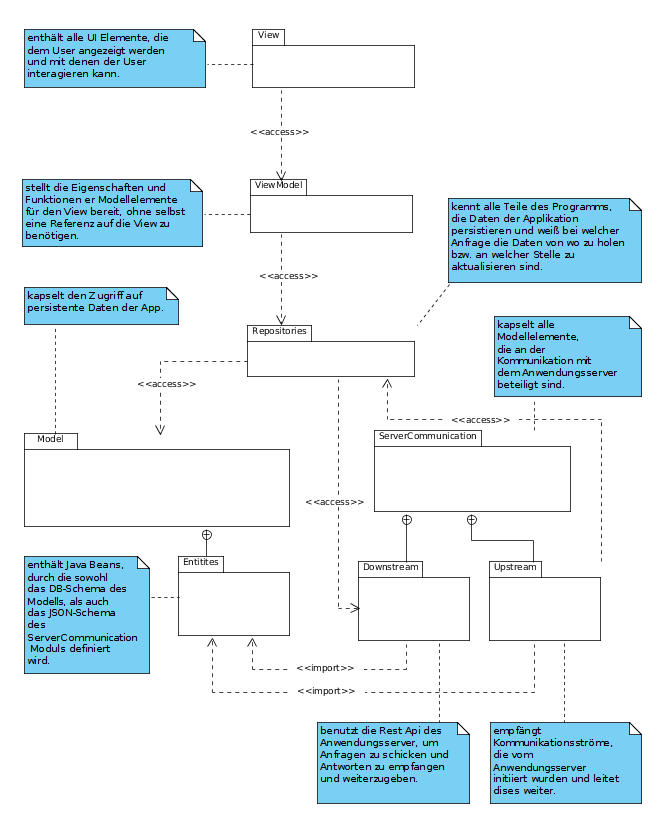
\includegraphics[scale=0.5]{../Klassendiagramme/paketdiagramm_client.png}
	\caption{Paketdiagramm der Clientanwendung}
\end{figure}

\subsubsection{Views}
Das Paket Views enthält alle Klassen, die am User Interface des Benutzers beteiligt sind. Das sind sämtliche Activities, Fragments und dazugehörige .xml-Layouts. Das Modul ist für die Präsentation der Appdaten sowie die Implementierung der Präsentationslogik (Umsetzung der Eigenschaften der Daten und Weiterleitung von Benutzereingaben) zuständig.

\textbf{Abhängigkeiten zu anderen Paketen:}\\
Das Paket Views kann die Informationen, die dem Benutzer angezeigt werden, nicht selbst generieren, sondern bekommt diese bereitgestellt von den entsprechenden ViewModells.

\textbf{Unterpakete:}\\
das Paket enthält das Unterpaket 'RecyclerView'. Da in der Applikation viele (verschiedene) RecyclerViews verwendet werden, gibt es für die Erstellung derselben ein eigenes Paket, dessen Aufgabe es ist, von den Datenobjekten die das Model liefert die gewünschten Informationen zu extrahieren und diese mit dem richtigen Layout zusammenzuführen. Innerhalb des Pakets besteht eine Abhängigkeit derjenigen View-Klassen, die einen RecyclerView verwenden zu dem Unterpaket RecyclerViews. Das Unterpaket RecyclerViews selbst ist nocht von anderen Klassen und Paketen abhängig.

\subsubsection{Modell}
Das Modell ist die Datenzugriffsschicht der Applikation, d.h. sie kapselt den Zugriff auf persistente Daten, die in einer lokalen SQLite Datenbank gehalten werden.Darüber hinaus enthält das Paket die Geschäftslogik der App, das hei?t hier werden die om ViewModel aufbereiteten und weitergeleiteten Befehle umgesetzt und anschließend die sich ergebenden Datenänderungen an das ViewModell zurückgegeben. Die Modellklassen, die sich lokal in der Applikation befinden, werden erweitert durch das Datenmodell, welches sich auf dem Server befindet. Es muss stets die Datenkonsistenz dieser zwei Modellteile sichergestellt werden (vgl. Paket Repository).

\textbf{Abhängigkeiten zu anderen Paketen}\\
Der Aufbau und die Operationen, die auf der lokalen Datenbank durchgeführt werden, werden mittels des Frameworks \textit{Room} realisiert.

\textbf{Unterpakete:}\\
Das Modell enthält das Unterpaket 'Entities'. Dies enthält die Java Entitäten, die von Room zu den Relationen der Datenbank umgesetzt werden. Die Datenbank kann von Room auch ohne eine Implementierung der Zugriffslogik aufgebaut werden. Die Entities haben demnach keine Anhängigkeiten zu anderen Klassen innerhalb des Programms. DIe Zugriffslogik der DAOs setzt hingegen die Existenz der Datenbank voraus, es gibt eine Abhängigkeit vom Modell zu den Entities.

\subsubsection{ViewModell}
Das ViewModell ist das Bindeglied zwischen View und Modell. Es tauscht Informationen mit dem Modell aus und stellt so der View öffentliche Eigenschaften und Befehle zur Verfügung, die an die Steuerungselemente der UI angebunden werden können. Dabei hat as ViewModell keine Referenz auf die View. Durch diese lose Kopplung kann die View jederzeit ausgetauscht werden, ohne dass das ViewModell verändert werden muss.

\textbf{Abhängigkeiten zu anderen Paketen}\\
Das ViewModell benötigt eine Referenz zum Modell, um die von der View empfangenen Befehle weiterleiten und die richtigen Daten von Modell anfordern zu können. Um diese Abhängigkeit zu entkoppeln und das Ansprechen der richtigen Modellkomponente zu erleichtern, wird diese Abhängigkeit über einen Vermittler ("Repository") geleitet. Dies ermöglicht das einfache Austauschen des Modells, ohne dass das ViewModell verändert werden muss.

\subsubsection{ServerCommunication}
Das Paket ServerCommunication übernimmt die Kommunikation der App mit dem Server, also das Speichern von Daten auf dem Server bzw. das Holen von Daten von dem Server. Darüber hinaus werden in diesem Paket auch Nachrichten, die vom Server gesendet werden empfangen und an das Modell zur Verarbeitung weitergeleitet.

\textbf{Abhängigkeiten zu anderen Paketen}\\
Das Paket hat keine Abhängigkeiten zu anderen Paketen der Applikation. Die Implementierung des REST-Clients erfolgt über das Framework \textit{Retrofit 2}. Hier besteht also eine Abhängigkeit zu einem externen Framework. Außerdem benötigt das Modukl zur fehlerfreien Ausführung seiner Aufgaben ein funktionierendes Backend (REST-Api, das die entsprechenden Ressourcen bereitstellt) des Systems.

\textbf{Unterpakete:}\\
Das Modul ServerCommunication setzt sich aus zwei Untermodulen zusammen. Das Modul \textit{Upstream} implementiert die Kommunikation, die über die REST-Api des Tomcat-Servers läuft, also jegliche Kommunikation, die von einem Client initiiert wird. Das Modul \textit{Downstream} hingegen ist dafür zuständig Kommunikationsströme zu empfangen, die vom Server initiiert werden und diese den Vermittlern zur Verbreitung weiterzuleiten.

\subsubsection{Repositories}
Wie in den vorherigen Abschnitten erläutert, ist die Geschäftslogik der App aufgeteilt auf den lokalen Teil (Modell) und einen Remote-Teil (ServerCommunication), die miteinander synchronisiert werden müssen. Zusätzlich müssen die ViewModells nach sämtlichen Änderungen mit den aktuellsten Daten versorgt werden. Dise Abhängigkeiten der einzelnen Komponenten werden in den Repository-Klassen zusammengefasst. Genauere Erläuterungen zur Funktionsweise finden sich in Abschnitt \ref{Vermittler}.

\textbf{Abhängigkeiten zu anderen Paketen:}\\
...

\subsection{Server}
Die Architektur ser Servers orientiert sich an einer Schichten-Architektur. Dabei handelt es sich nicht um eine klassische Schichtenarchitektur, bei der nur obere Schichten Dienste der unteren Schichten aufrufen darf. Stattdessen sind die oberen Schichten in zwei Unterpakete unterteilt. In einer Hälfte jeder Schicht gehen die Methodenaufrufe von oben nach unten, in der anderen von unten nach oben. Durch diese zwei Säulen in der Anwendung ist die Implementierung, trotz Verletzung des Schichtenmodells, leicht realisierbar, da die Unterpakete immernoch topologisch sortiebar sind, sodass
eine Implementierungsreihenfolge gefunden werden kann, bei der zu jeder Zeit die Abhängigkeiten des gerade entwickelten Moduls bereits implementiert sind.

\begin{figure}[H]
	\centering
	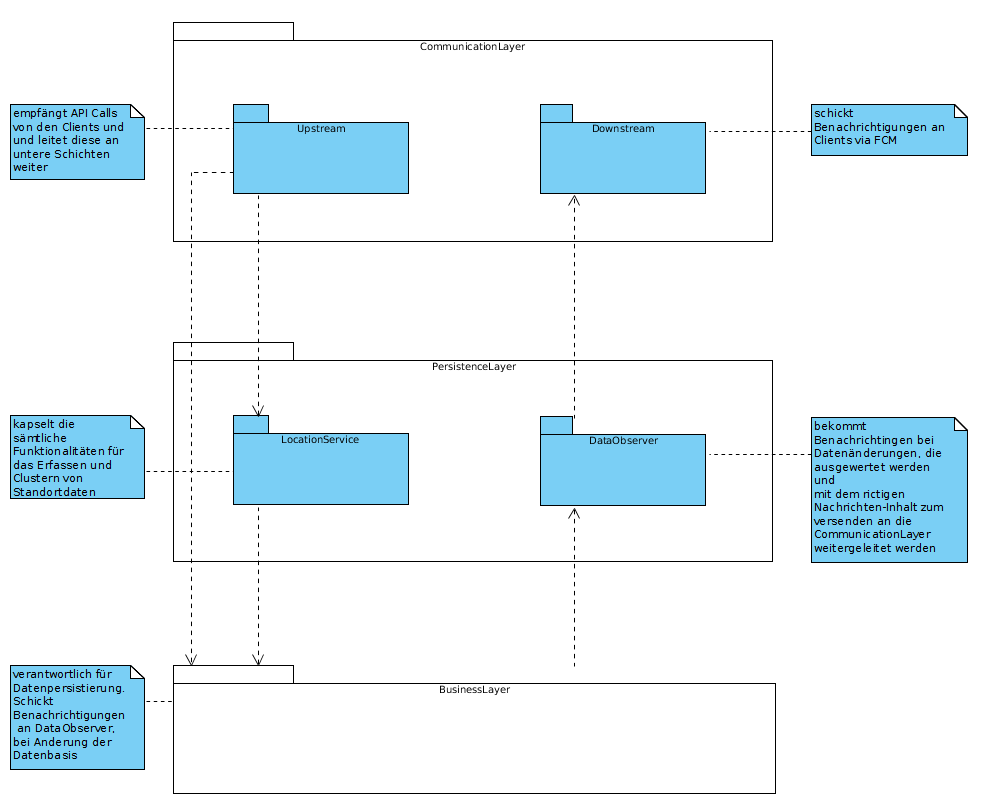
\includegraphics[scale=0.5]{../Klassendiagramme/paketdiagramm_server.png}
	\caption{Paketdiagramm der Clientanwendung}
\end{figure}

Das Programm des Servers ist in folgende Pakete aufgeteilt:
\begin{itemize}
	\item CommunicationLayer
	\item BusinessLayer
	\item PersistenceLayer
\end{itemize}

\subsubsection{CommunicationLayer}
Dieses Paket bildet die oberste Schicht der Serveranwendung und ist die einzige Schicht, die für die Clients sichtbar ist. Die CommunicationLayer vereint alle Klassen, die an der Kommunikation mit den Clients beteiligt sind. Es besteht aus den Unterpaketn Upstream und Downstream. Die Klassen des Pakets Upstream sind dafür zuständig, ein REST-API zur Verfügung zu stellen und auf Anfragen der Clients zu antworten, d.h. die Kommunikation wird von den Clients initiiert. Das Downstream-Paket hingegen schickt Nachrichten an Clients, ohne vorher von diesen angesprochen worden zu sein. Hierf"ur wird der Firebase Cloud Messaging Service benutzt.

Das Untermodul Upstream nimmt die Dineste der unteren Schichten in Anspruch. Dabei handelt es sich um eine transparente Schichtenarchitektur, das bedeutet das Modul nimmt nicht nur die Dienste der mittleren, sondern auch die Dienste der unteren Schicht in Anspruch.

Das Untermodul Downstream hingegen bietet Dienste an, nämlich das versenden von Nachrichten an Clients, die von den unteren Schichten der Serverandwendung verwendet wird.

\subsubsection{BusinessLayer}
Die BusinessLayer ist die mittlere Schicht und beinhaltet den Großteil der Anwendungslogik der Serveranwendung. Wie die anderen Schichten des Server, besteht auch die BusinessLayer aus zwei Untermodulen: LocationService und DataObserver.

Das Modul LocationService kümmert sich um alle Angelegenheiten, die mit der Erfassung, der kurzzeitigen Persistierung und dem Clustering von Standortdaten zusammenhängen. Dieser Dienst wird von der oberen Schicht in Anspruch genommen. Zur unteren Schicht bestehen keine Abhängigkeiten, da Standortdaten nicht in der datenbank gespeichert weden. Dieses Untermodul aht selbst also keine Abhängigkeiten zu anderen Paketen.

Das zweite Untermodul der BusinessLayer ist das DataObserver-Modul. Dieses Modul wird bei Anderungen in der Datenbasis von der PersistenceLayer angesprochen und kümmert sich folgend darum, die Änderungen zu analysieren, herauszufinden welche Clients von der Änderung erfahren müssen und diese Informationen an die obere Schicht weiterzuleiten, um eine Nachricht an genau diese Clients zu schicken. Dementsrechend bietet dieses Untermodul einen Dienst, der von der PersistenceLayer in Anspruch genommen wird und nimmt einen Dienst in Ansprcu der von der CommunicationLayer angeboten wird.

\subsubsection{PersistenceLayer}
Die PersistenceLayer kapselt das Datenmodellder Anwendung in sich. Sie ist für die Speicherung der Daten zuständig, sowie für die Weiterleitung der Daten an die Communicationlayer und somit an die Clients. Die PersistenceLayer setzt sich zusammen aus einer MySQL-Datenbank, die mit dem ORM-Framework Hibernate verwaltet wird und DAO-Klassen, in denen die Datenbankzugriffe gekapselt werden.

Im Gegensatz zu den zwei anderen Schichten gibt es in dieser Schicht keine Untermodule. Der Dienst des Moduls wird von dem Upstream-Modul der CommunicationLayer in Anspruch genommen. Geschieht dies, wird aus der PersistenceLayer der Dienst der DataObserver angestoßen, um die Änderungen in dem Datenbestand wieder durch die Schichten nach oben und schließlich zu den Clients zu leiten.

\newpage


\section{verwendete Entwurfsmuster}

\subsection{Schablonenmethode für SignInHelper}
Die verschiedenen Anmelde-Aktivitäten aller Loginhelper-Klassen können über die signIn()-Methode angesto"sen werden. Der spezifische Ablauf der Anmelde-Aktivität wird in den Unterklassen durch die primitiven Methoden definiert. \\

\textbf{beteiligte Klassen:}
\begin{itemize}
	\item SignInHelper: besitzt die Methode signIn(), die als Schablonenmethode dient und bei der Ausführung die primitiven Methoden configureSignIn() und startSignInProcess() aufruft
	\item FirebaseSignInHelper: Unterklasse von SignInHelper, die die primitiven Methoden configureSignIn() und startSignInProcess() implementiert
	\item GoSignInHelper: Unterklasse von SignInHelper, die die primitiven Methoden configureSignIn() und startSignInProcess() implementiert
\end{itemize}

\subsection{Beobachter zum Aktualisieren des UI}
Durch das Ausführen von Befehlen von einem Benutzer, kann es zu Änderungen in den Daten kommen, die eine Änderung des aktuellen Views anderer Benutzer erfordern. Diese 1-zu-n Abhängigkeit wird durch ein Beobachter-muster behandelt. Die dafür benötigte Funktionalität wird von der Architecture-Components Framework Klasse LiveData<> bereitgestellt. Ein Objekt dieser Klasse kann von einem LifeCycleOwner (z.B. eine Lifecycle-Activity oder ein LifecycleFragment) beobachtet werden und löst bei Änderung den Methodenaufruf \textit{onChanged()} aus. Die Livedata-Objekte sind Lifecycle-Aware, das bedeutet eine Benachrichtigung über eine Änderung wird nur dann an einen Beobachter weitergeleitet, wenn er sich in einem aktiven Stadium seines Lifecycles befindet.\\
\textbf{beteiligte Klassen:}
\begin{itemize}
	\item \textit{LiveData<>:}\\ das beobachtete Subjekt
	\item \textit{BaseActivity (die von LifecycleActivity erbt):}\\ Der Beobachter, der bei Änderung der Daten benachrichtigt wird und daraufhin das dem Benutzer präsentierte UI aktualisiert.
\end{itemize}

\subsection{Beobachter zum Weiterleiten von Änderungen der Datenbasis}
Werden von einem Client Daten der App geändret (z.B. eine GO erstellt, ein Benutzer zu einer Gruppe hinzugefügt) betrifft dies in vielen auch die Daten, die ein anderer Client bei sich gespeichert hat und benutzt. Dementsprechend müssen Clients vom Server über Änderungen in der DAtenbasis informaiert werden können. Es ergibt sich eine 1-zu-n-Abhängigkeit: n Clients sind von 1 Datenbasis abhängig.

Zur Auflösung dieser Abhängigkeit wird in der Anwendung eine Beobachter-Muster verwendet. Die Datenbasis wird beobachtet und bei Änderungen leiten die Beobachter die Benachrichtigung der Clients
ein. Da ein Beobachter nicht ein einzelnes Objekt, sondern eine gesamte Datenbanktabelle beobachet, ist es schwierig, den aktuellen Zustand des Subjekts im Beobachter zu speichern. Aus idesem Grund verwenden die beobachter eine push-Methodik, bei der die Änderungen bei der Benachrichtigung der Beobachter mit übergeben werden.

\textbf{beteiligte Klassen:}
\begin{itemize}
	\item \textit{Observable<T>}\\ Das Interface ist das abstrakte Subjekt. Jedes konkrete Subjekt muss dieses Interface und damit die Methode notify() implementieren. Diese Methode benachrichtigt die Beobachter über ein Update in der Datenbasis.
	\item \textit{DAO-Klassen}\\ Diese Klassen implementieren das Interface Observable und sind die konkreten Subjekte, die von den Beobachtern beobachtet werden.
	\item \textit{Observer}\\ Das Interface Observer ist der abstrakte Beobachter. Jeder konkrete Beobachter muss dieses Interface und damit die Methode update() implementieren.
	\item \textit{EntityObserver}\\Konkrete Beobachter, die das Interface Observer implementieren. Jede dieser Klassen übernimmt die Verantwortung für bestimmte Änderungen in der Datenbasis, analysiert, welche Änderung geschehen ist und übergibt diese Daten zum versenden an den FcmClient.
\end{itemize}

\subsection{DAO-Pattern zur Persistierung von Daten}
Die Daten der App werden in eine MySQL-Datenbank persistiert. Für den Zugriff auf diese Datenbank wird ein Data Access Object Entwurfsmuster verwendet. Dabei werden zum Einen Java Beans verwendet, die die Struktur der Datenbankrelationen festlegen. Zum Anderen gibt es spezielle DAO-Klassen die alle Datenbankzugriffe in sich kapseln. So können zusätzliche Zugriffsmethoden für die Datenbank hinzugefügt werden, ohne die Entity-Klassen verändern zu müssen. Andersherum kann der Aufbau der Datenbank verändert werden, ohne dass die DAO-klasseni ihre Schnittstelle nach außen verändern.
Die Umsetzung der Datenbank und der SQL-Queries wird mithilfe des Frameworks Hibernate realisiert.\\

\textbf{beteiligte Klassen:}
\begin{itemize}
	\item \textit{UserEntity, GoEntity, GroupEntity}\\ Entity-Beans, die die Struktur der Datenbankrelationen darstellen
	\item \textit{AbstractDAO}\\ INterface für eine DAO-Klasse, wleches Zugriffsmethoden definiert, die auf jeder Datenbanktabelle durchgeführt werden müssen (CRUD)
	\item \textit{UserDao, GoDao, GroupDao}\\ Data-Access-Object Interfaces, die spezielle Zugriffsmethoden enthalten, die nur für bestimmte Datenbanktabellen gebraucht werden.
	\item \textit{UserDaoImp, GoDapImp, GroupDaoImp}\\ konkrete IMplementierungen der DAO Interfaces. Hier werden die Zugriffsmethoden anhand des von den Entity-Klassen definierten Datenbankschemas
	implementiert.
\end{itemize}

\subsection{Vermittler zur Koordination von Datenzugriffen}\label{Vermittler}
Viele Apps Nutzen eine lokale Datenbank, um eine Benutzung der App, zumindest ansatzweise, auch ohne Internetverbindung zu ermöglichen. Auch wenn in diesem Entwurf keine lokale Datenbank auf den CLients vorgesehen ist, soll dieses Feature leicht erweiterbar sein. Zu diesem Zweck ist bei der Aktualisierung/Beschaffung der Daten für die ViewModels eine zusätzliche Indirektionsstufe eingebaut: Die Repositories. Diese übernehmen im Zusammenspiel der App-Komponenten eine Vermittler-Funktion: Während die ViewModels wissen WAS gemacht werden muss (da diese die aktuellen Daten und Funktionen für den User speichern), wissen die Repositories WO dies getan werden muss - in der lokalen Datenbank, in den SharedPreferences des Andorid-Geräts oder auf dem Remote Server.

\textbf{beteiligte Klassen:}
\begin{itemize}
	\item \textit{GoRepositor, GroupRepository, UserRepository:}\\
	 Die Vermittler die die Koordination der Kollegen übernehmen
	\item \textit{ViewModell, TomcatRestApi, lokale Datenbank, SharedPreferences:}\\ Kollegen, die nichts voneinander wissen, sondern bei allen Aufrufen vom vermittler angesprochen werden, bzw. den Vermittler ansprechen.
\end{itemize}

\subsection{Strategiemuster zur Kapselung des Clustering-Alogithmus}
Das Clustern der Standorte der Teilnehmer eines GOs wird von der Klasse GoClusterStrategy übernommen. Diese Klasse ist mittels eines Strategy-Patterns in das Programm eingebunden. Dies entkoppelt den Algorithmus von seinem Kontext und erkann dynamisch durch andere Clustering-Alogirthmen ersetzt oder ergänzt werden. \\

\textbf{beteiligte Klassen:}
\begin{itemize}
	\item \textit{LocationService} \\
	Die Klasse ist der Kontext der Clustering-Strategie. Von hier aus wird die Ausführung des Algorithmus angestoßen.
	\item \textit{ClusterStrategy} \\
	ClusterStrategy ist ein Interface, das von jedem Cluster-Algorithmus implementiert werden muss. Es definiert eine \textit{caluculateCluster()} Methode, die eine Liste an einzelnen User-Standorten entgegen nimmt und eine Liste an User-Clustern zurückgibt.
	\item \textit{GoClusterStrategy} \\
	In dieser Klasse wird der Clustering-Algorithmus implementiert, der angewendet werden soll. Die Klasse erweitert das Interface ClusterStrategy.
\end{itemize}

\subsection{Fassade zur Vereinfachung des Server Interfaces}
Der verwendete Tomcat-Server bietet seinem Clients zur Kommunikation ein REST Interface an. Das Ansprechen der verschiedenen REST Ressourcen ist in der App hinter dem Interface \textit{TomcatRestApi}. Das Interface bietet den aufrufenden Klassen Methoden zum aufrufen der REST Ressourcen an, ohne das ein Aufrufer etwas von der eigentlichen Kommunikation mit dem Server wissen muss. \\

\textbf{beteiligte Klassen}
\begin{itemize}
	\item \textit{TomcatRestApi} \\
	Das Interface ist die Fassade, die die Schnittstelle zum Tomcat-Server hinter sich versteckt. Nach außen werden Methoden bereitgestellt, die von anderen Klassen aufgerufen werden können, um Server-Dienste in Anspruch nehmen zu können, ohne sich um die Details der Kommunikation zu kümmern.
\end{itemize}

\subsection{Dekorierer zur Erweiterung der Aktivitäten für Sonderbenutzer}
Für GO-Verantwortliche und Gruppenadmins werden GroupDetailActivity oder GoDetailActivity entschprechend erweitert. Zusätzliche Buttons und Methoden werden hinzugefügt.(z.B. Name der Gruppe ändern, Mitglieder hinzufügen usw.) Dazu haben wir eine Android-Version von Dekorierer benutzt. Die spezielle Unterklassen (GroupDetailActivitzOwner bzw. GoDetailActivityOwner) von oben genannten Activities benutzen fertige Oberklassen Activities und fügen darauf die benötigte Funktionalität hinzu.

\textbf{beteiligte Klassen}
\begin{itemize}
\item \textit{GroupdetailActivity} \\
Activity, wo die Gruppendetails angezeigt werden. Ist eine Oberklasse von GroupDetailActivityOwner.
\item \textit{GroupDetailActivityOwner}
Erweitert die Oberklasse um Funktionen für die Admins.
\item \textit{GoDetailActivity}
Activity, wo Go-Details angezeigt werden. Oberklasse von GoDetailActivityOwner.
\item \textit{GoDetailActivityOwner}
Erweitert die Oberklasse um Funktionen für den GO-Verantwortlichen
\end{itemize}


\subsection{Command Muster zur Bearbeitung der Server Messages auf der Client Seite}


\newpage

\section{Client-Server-Schnittstelle}
Dieser Abschnitt erläutert die Schnittstelle zwischen dem Client und dem Server. Diese Schnittstelle besteht aus zwei Teilen:

Zum Einen bietet der Server eine REST API an, über die der Client die Dienste des Servers in Anspruch nehmen kann. Zum Anderen gibt es eine Schnittstelle, die über Firebase Cloud Messaging realisiert ist, damit der Server Nachrichten an bestimmte Clients schicken kann.

\subsection{REST API des Servers}



\section{Klassenbeschreibungen}

% ------- textdoclet_include/intro.tex end

\section*{Class Hierarchy}{
\thispagestyle{empty}
\markboth{Class Hierarchy}{Class Hierarchy}
\addcontentsline{toc}{section}{Class Hierarchy}
\subsection*{Classes}
{\raggedright
\hspace{0.0cm} $\bullet$ java.lang.Object {\tiny \refdefined{java.lang.Object}} \\
\hspace{1.0cm} $\bullet$ edu.kit.pse17.go\_app.ClientCommunication.Downstream.FcmClient {\tiny \refdefined{edu.kit.pse17.go_app.ClientCommunication.Downstream.FcmClient}} \\
\hspace{1.0cm} $\bullet$ edu.kit.pse17.go\_app.ClientCommunication.Upstream.GoRestController {\tiny \refdefined{edu.kit.pse17.go_app.ClientCommunication.Upstream.GoRestController}} \\
\hspace{1.0cm} $\bullet$ edu.kit.pse17.go\_app.ClientCommunication.Upstream.GroupRestController {\tiny \refdefined{edu.kit.pse17.go_app.ClientCommunication.Upstream.GroupRestController}} \\
\hspace{1.0cm} $\bullet$ edu.kit.pse17.go\_app.ClientCommunication.Upstream.UserRestController {\tiny \refdefined{edu.kit.pse17.go_app.ClientCommunication.Upstream.UserRestController}} \\
\hspace{1.0cm} $\bullet$ edu.kit.pse17.go\_app.Main {\tiny \refdefined{edu.kit.pse17.go_app.Main}} \\
\hspace{1.0cm} $\bullet$ edu.kit.pse17.go\_app.PersistenceLayer.GoEntity {\tiny \refdefined{edu.kit.pse17.go_app.PersistenceLayer.GoEntity}} \\
\hspace{1.0cm} $\bullet$ edu.kit.pse17.go\_app.PersistenceLayer.GroupEntity {\tiny \refdefined{edu.kit.pse17.go_app.PersistenceLayer.GroupEntity}} \\
\hspace{1.0cm} $\bullet$ edu.kit.pse17.go\_app.PersistenceLayer.UserEntity {\tiny \refdefined{edu.kit.pse17.go_app.PersistenceLayer.UserEntity}} \\
\hspace{1.0cm} $\bullet$ edu.kit.pse17.go\_app.PersistenceLayer.daos.GoDaoImp {\tiny \refdefined{edu.kit.pse17.go_app.PersistenceLayer.daos.GoDaoImp}} \\
\hspace{1.0cm} $\bullet$ edu.kit.pse17.go\_app.PersistenceLayer.daos.GroupDaoImp {\tiny \refdefined{edu.kit.pse17.go_app.PersistenceLayer.daos.GroupDaoImp}} \\
\hspace{1.0cm} $\bullet$ edu.kit.pse17.go\_app.PersistenceLayer.daos.UserDaoImp {\tiny \refdefined{edu.kit.pse17.go_app.PersistenceLayer.daos.UserDaoImp}} \\
\hspace{1.0cm} $\bullet$ edu.kit.pse17.go\_app.ServiceLayer.Cluster {\tiny \refdefined{edu.kit.pse17.go_app.ServiceLayer.Cluster}} \\
\hspace{1.0cm} $\bullet$ edu.kit.pse17.go\_app.ServiceLayer.EntitiyRemovedObserver {\tiny \refdefined{edu.kit.pse17.go_app.ServiceLayer.EntitiyRemovedObserver}} \\
\hspace{1.0cm} $\bullet$ edu.kit.pse17.go\_app.ServiceLayer.EntityAddedObserver {\tiny \refdefined{edu.kit.pse17.go_app.ServiceLayer.EntityAddedObserver}} \\
\hspace{1.0cm} $\bullet$ edu.kit.pse17.go\_app.ServiceLayer.EntityChangedObserver {\tiny \refdefined{edu.kit.pse17.go_app.ServiceLayer.EntityChangedObserver}} \\
\hspace{1.0cm} $\bullet$ edu.kit.pse17.go\_app.ServiceLayer.GoClusterStrategy {\tiny \refdefined{edu.kit.pse17.go_app.ServiceLayer.GoClusterStrategy}} \\
\hspace{1.0cm} $\bullet$ edu.kit.pse17.go\_app.ServiceLayer.LocationService {\tiny \refdefined{edu.kit.pse17.go_app.ServiceLayer.LocationService}} \\
\hspace{1.0cm} $\bullet$ edu.kit.pse17.go\_app.ServiceLayer.UserLocation {\tiny \refdefined{edu.kit.pse17.go_app.ServiceLayer.UserLocation}} \\
\hspace{1.0cm} $\bullet$ java.lang.Enum {\tiny \refdefined{java.lang.Enum}} \\
\hspace{2.0cm} $\bullet$ edu.kit.pse17.go\_app.ClientCommunication.Downstream.EventArg {\tiny \refdefined{edu.kit.pse17.go_app.ClientCommunication.Downstream.EventArg}} \\
\hspace{2.0cm} $\bullet$ edu.kit.pse17.go\_app.PersistenceLayer.Status {\tiny \refdefined{edu.kit.pse17.go_app.PersistenceLayer.Status}} \\
}
\subsection*{Interfaces}
\hspace{0.0cm} $\bullet$ edu.kit.pse17.go\_app.PersistenceLayer.daos.AbstractDao {\tiny \refdefined{edu.kit.pse17.go_app.PersistenceLayer.daos.AbstractDao}} \\
\hspace{0.0cm} $\bullet$ edu.kit.pse17.go\_app.PersistenceLayer.daos.GoDao {\tiny \refdefined{edu.kit.pse17.go_app.PersistenceLayer.daos.GoDao}} \\
\hspace{0.0cm} $\bullet$ edu.kit.pse17.go\_app.PersistenceLayer.daos.GroupDao {\tiny \refdefined{edu.kit.pse17.go_app.PersistenceLayer.daos.GroupDao}} \\
\hspace{0.0cm} $\bullet$ edu.kit.pse17.go\_app.PersistenceLayer.daos.UserDao {\tiny \refdefined{edu.kit.pse17.go_app.PersistenceLayer.daos.UserDao}} \\
\hspace{0.0cm} $\bullet$ edu.kit.pse17.go\_app.ServiceLayer.ClusterStrategy {\tiny \refdefined{edu.kit.pse17.go_app.ServiceLayer.ClusterStrategy}} \\
\hspace{0.0cm} $\bullet$ edu.kit.pse17.go\_app.ServiceLayer.Observable {\tiny \refdefined{edu.kit.pse17.go_app.ServiceLayer.Observable}} \\
\hspace{0.0cm} $\bullet$ edu.kit.pse17.go\_app.ServiceLayer.Observer {\tiny \refdefined{edu.kit.pse17.go_app.ServiceLayer.Observer}} \\
}
\section{Package edu.kit.pse17.go\_app.PersistenceLayer}{
\label{edu.kit.pse17.go_app.PersistenceLayer}\hypertarget{edu.kit.pse17.go_app.PersistenceLayer}{}
\hskip -.05in
\hbox to \hsize{\textit{ Package Contents\hfil Page}}
\vskip .13in
\hbox{{\bf  Classes}}
\entityintro{GoEntity}{edu.kit.pse17.go_app.PersistenceLayer.GoEntity}{Dies ist eine Entity Klasse.}
\entityintro{GroupEntity}{edu.kit.pse17.go_app.PersistenceLayer.GroupEntity}{Dies ist eine Entity Klasse.}
\entityintro{Status}{edu.kit.pse17.go_app.PersistenceLayer.Status}{Dieses Enum definiert die verschiedenen Teilnahmestati, die ein Benutzer in einem GO innehaben kann.}
\entityintro{UserEntity}{edu.kit.pse17.go_app.PersistenceLayer.UserEntity}{Dies ist eine Entity Klasse.}
\vskip .1in
\vskip .1in
\subsection{\label{edu.kit.pse17.go_app.PersistenceLayer.GoEntity}Class GoEntity}{
\hypertarget{edu.kit.pse17.go_app.PersistenceLayer.GoEntity}{}\vskip .1in 
Dies ist eine Entity Klasse. Sie wird von dem Framework Hinbernate dazu verwendet, POJOS auf Tupel in einer Datenbank zu mappen. Wie das Mapping geschieht ist in dieser Klasse durch Annotations festgelegt. Der Rest der Anwendung kann somit überall mit Java-Objekten hantieren und muss sich nicht um die konkrete Implementierung der Datenbank kümmern. Der Zugriff auf die Datenbank erfolgt nicht in dieser Klasse, sondern nur über eine DAO Klasse, die das Interface GoDao implementiert. Zusätzlich dient diese Klasse als Vorlage des Frameworks Gson zum Parsen von JSON-Objekten, die von der REST API empfangen und gesendet werden. Die Attribute der Klasse bestimmen dabei die Struktur des JSON-Objekts.\vskip .1in 
\subsubsection{Declaration}{
\begin{lstlisting}[frame=none]
public class GoEntity
 extends java.lang.Object\end{lstlisting}
\subsubsection{Constructor summary}{
\begin{verse}
\hyperlink{edu.kit.pse17.go_app.PersistenceLayer.GoEntity()}{{\bf GoEntity()}} \\
\end{verse}
}
\subsubsection{Method summary}{
\begin{verse}
\hyperlink{edu.kit.pse17.go_app.PersistenceLayer.GoEntity.equals(java.lang.Object)}{{\bf equals(Object)}} \\
\hyperlink{edu.kit.pse17.go_app.PersistenceLayer.GoEntity.getDescription()}{{\bf getDescription()}} \\
\hyperlink{edu.kit.pse17.go_app.PersistenceLayer.GoEntity.getEnd()}{{\bf getEnd()}} \\
\hyperlink{edu.kit.pse17.go_app.PersistenceLayer.GoEntity.getGoingUsers()}{{\bf getGoingUsers()}} \\
\hyperlink{edu.kit.pse17.go_app.PersistenceLayer.GoEntity.getGoneUsers()}{{\bf getGoneUsers()}} \\
\hyperlink{edu.kit.pse17.go_app.PersistenceLayer.GoEntity.getID()}{{\bf getID()}} \\
\hyperlink{edu.kit.pse17.go_app.PersistenceLayer.GoEntity.getLat()}{{\bf getLat()}} \\
\hyperlink{edu.kit.pse17.go_app.PersistenceLayer.GoEntity.getLon()}{{\bf getLon()}} \\
\hyperlink{edu.kit.pse17.go_app.PersistenceLayer.GoEntity.getName()}{{\bf getName()}} \\
\hyperlink{edu.kit.pse17.go_app.PersistenceLayer.GoEntity.getNotGoingUsers()}{{\bf getNotGoingUsers()}} \\
\hyperlink{edu.kit.pse17.go_app.PersistenceLayer.GoEntity.getStart()}{{\bf getStart()}} \\
\hyperlink{edu.kit.pse17.go_app.PersistenceLayer.GoEntity.hashCode()}{{\bf hashCode()}} \\
\hyperlink{edu.kit.pse17.go_app.PersistenceLayer.GoEntity.setDescription(java.lang.String)}{{\bf setDescription(String)}} \\
\hyperlink{edu.kit.pse17.go_app.PersistenceLayer.GoEntity.setEnd(java.util.Date)}{{\bf setEnd(Date)}} \\
\hyperlink{edu.kit.pse17.go_app.PersistenceLayer.GoEntity.setGoingUsers(java.util.List)}{{\bf setGoingUsers(List)}} \\
\hyperlink{edu.kit.pse17.go_app.PersistenceLayer.GoEntity.setGoneUsers(java.util.List)}{{\bf setGoneUsers(List)}} \\
\hyperlink{edu.kit.pse17.go_app.PersistenceLayer.GoEntity.setID(long)}{{\bf setID(long)}} \\
\hyperlink{edu.kit.pse17.go_app.PersistenceLayer.GoEntity.setLat(long)}{{\bf setLat(long)}} \\
\hyperlink{edu.kit.pse17.go_app.PersistenceLayer.GoEntity.setLon(long)}{{\bf setLon(long)}} \\
\hyperlink{edu.kit.pse17.go_app.PersistenceLayer.GoEntity.setName(java.lang.String)}{{\bf setName(String)}} \\
\hyperlink{edu.kit.pse17.go_app.PersistenceLayer.GoEntity.setNotGoingUsers(java.util.List)}{{\bf setNotGoingUsers(List)}} \\
\hyperlink{edu.kit.pse17.go_app.PersistenceLayer.GoEntity.setStart(java.util.Date)}{{\bf setStart(Date)}} \\
\end{verse}
}
\subsubsection{Constructors}{
\vskip -2em
\begin{itemize}
\item{ 
\index{GoEntity()}
\hypertarget{edu.kit.pse17.go_app.PersistenceLayer.GoEntity()}{{\bf  GoEntity}\\}
\begin{lstlisting}[frame=none]
public GoEntity()\end{lstlisting} %end signature
}%end item
\end{itemize}
}
\subsubsection{Methods}{
\vskip -2em
\begin{itemize}
\item{ 
\index{equals(Object)}
\hypertarget{edu.kit.pse17.go_app.PersistenceLayer.GoEntity.equals(java.lang.Object)}{{\bf  equals}\\}
\begin{lstlisting}[frame=none]
public boolean equals(java.lang.Object arg0)\end{lstlisting} %end signature
}%end item
\item{ 
\index{getDescription()}
\hypertarget{edu.kit.pse17.go_app.PersistenceLayer.GoEntity.getDescription()}{{\bf  getDescription}\\}
\begin{lstlisting}[frame=none]
public java.lang.String getDescription()\end{lstlisting} %end signature
}%end item
\item{ 
\index{getEnd()}
\hypertarget{edu.kit.pse17.go_app.PersistenceLayer.GoEntity.getEnd()}{{\bf  getEnd}\\}
\begin{lstlisting}[frame=none]
public java.util.Date getEnd()\end{lstlisting} %end signature
}%end item
\item{ 
\index{getGoingUsers()}
\hypertarget{edu.kit.pse17.go_app.PersistenceLayer.GoEntity.getGoingUsers()}{{\bf  getGoingUsers}\\}
\begin{lstlisting}[frame=none]
public java.util.List getGoingUsers()\end{lstlisting} %end signature
}%end item
\item{ 
\index{getGoneUsers()}
\hypertarget{edu.kit.pse17.go_app.PersistenceLayer.GoEntity.getGoneUsers()}{{\bf  getGoneUsers}\\}
\begin{lstlisting}[frame=none]
public java.util.List getGoneUsers()\end{lstlisting} %end signature
}%end item
\item{ 
\index{getID()}
\hypertarget{edu.kit.pse17.go_app.PersistenceLayer.GoEntity.getID()}{{\bf  getID}\\}
\begin{lstlisting}[frame=none]
public long getID()\end{lstlisting} %end signature
}%end item
\item{ 
\index{getLat()}
\hypertarget{edu.kit.pse17.go_app.PersistenceLayer.GoEntity.getLat()}{{\bf  getLat}\\}
\begin{lstlisting}[frame=none]
public long getLat()\end{lstlisting} %end signature
}%end item
\item{ 
\index{getLon()}
\hypertarget{edu.kit.pse17.go_app.PersistenceLayer.GoEntity.getLon()}{{\bf  getLon}\\}
\begin{lstlisting}[frame=none]
public long getLon()\end{lstlisting} %end signature
}%end item
\item{ 
\index{getName()}
\hypertarget{edu.kit.pse17.go_app.PersistenceLayer.GoEntity.getName()}{{\bf  getName}\\}
\begin{lstlisting}[frame=none]
public java.lang.String getName()\end{lstlisting} %end signature
}%end item
\item{ 
\index{getNotGoingUsers()}
\hypertarget{edu.kit.pse17.go_app.PersistenceLayer.GoEntity.getNotGoingUsers()}{{\bf  getNotGoingUsers}\\}
\begin{lstlisting}[frame=none]
public java.util.List getNotGoingUsers()\end{lstlisting} %end signature
}%end item
\item{ 
\index{getStart()}
\hypertarget{edu.kit.pse17.go_app.PersistenceLayer.GoEntity.getStart()}{{\bf  getStart}\\}
\begin{lstlisting}[frame=none]
public java.util.Date getStart()\end{lstlisting} %end signature
}%end item
\item{ 
\index{hashCode()}
\hypertarget{edu.kit.pse17.go_app.PersistenceLayer.GoEntity.hashCode()}{{\bf  hashCode}\\}
\begin{lstlisting}[frame=none]
public native int hashCode()\end{lstlisting} %end signature
}%end item
\item{ 
\index{setDescription(String)}
\hypertarget{edu.kit.pse17.go_app.PersistenceLayer.GoEntity.setDescription(java.lang.String)}{{\bf  setDescription}\\}
\begin{lstlisting}[frame=none]
public void setDescription(java.lang.String description)\end{lstlisting} %end signature
}%end item
\item{ 
\index{setEnd(Date)}
\hypertarget{edu.kit.pse17.go_app.PersistenceLayer.GoEntity.setEnd(java.util.Date)}{{\bf  setEnd}\\}
\begin{lstlisting}[frame=none]
public void setEnd(java.util.Date end)\end{lstlisting} %end signature
}%end item
\item{ 
\index{setGoingUsers(List)}
\hypertarget{edu.kit.pse17.go_app.PersistenceLayer.GoEntity.setGoingUsers(java.util.List)}{{\bf  setGoingUsers}\\}
\begin{lstlisting}[frame=none]
public void setGoingUsers(java.util.List goingUsers)\end{lstlisting} %end signature
}%end item
\item{ 
\index{setGoneUsers(List)}
\hypertarget{edu.kit.pse17.go_app.PersistenceLayer.GoEntity.setGoneUsers(java.util.List)}{{\bf  setGoneUsers}\\}
\begin{lstlisting}[frame=none]
public void setGoneUsers(java.util.List goneUsers)\end{lstlisting} %end signature
}%end item
\item{ 
\index{setID(long)}
\hypertarget{edu.kit.pse17.go_app.PersistenceLayer.GoEntity.setID(long)}{{\bf  setID}\\}
\begin{lstlisting}[frame=none]
public void setID(long ID)\end{lstlisting} %end signature
}%end item
\item{ 
\index{setLat(long)}
\hypertarget{edu.kit.pse17.go_app.PersistenceLayer.GoEntity.setLat(long)}{{\bf  setLat}\\}
\begin{lstlisting}[frame=none]
public void setLat(long lat)\end{lstlisting} %end signature
}%end item
\item{ 
\index{setLon(long)}
\hypertarget{edu.kit.pse17.go_app.PersistenceLayer.GoEntity.setLon(long)}{{\bf  setLon}\\}
\begin{lstlisting}[frame=none]
public void setLon(long lon)\end{lstlisting} %end signature
}%end item
\item{ 
\index{setName(String)}
\hypertarget{edu.kit.pse17.go_app.PersistenceLayer.GoEntity.setName(java.lang.String)}{{\bf  setName}\\}
\begin{lstlisting}[frame=none]
public void setName(java.lang.String name)\end{lstlisting} %end signature
}%end item
\item{ 
\index{setNotGoingUsers(List)}
\hypertarget{edu.kit.pse17.go_app.PersistenceLayer.GoEntity.setNotGoingUsers(java.util.List)}{{\bf  setNotGoingUsers}\\}
\begin{lstlisting}[frame=none]
public void setNotGoingUsers(java.util.List notGoingUsers)\end{lstlisting} %end signature
}%end item
\item{ 
\index{setStart(Date)}
\hypertarget{edu.kit.pse17.go_app.PersistenceLayer.GoEntity.setStart(java.util.Date)}{{\bf  setStart}\\}
\begin{lstlisting}[frame=none]
public void setStart(java.util.Date start)\end{lstlisting} %end signature
}%end item
\end{itemize}
}
}
\subsection{\label{edu.kit.pse17.go_app.PersistenceLayer.GroupEntity}Class GroupEntity}{
\hypertarget{edu.kit.pse17.go_app.PersistenceLayer.GroupEntity}{}\vskip .1in 
Dies ist eine Entity Klasse. Sie wird von dem Framework Hinbernate dazu verwendet, POJOS auf Tupel in einer Datenbank zu mappen. Wie das Mapping geschieht ist in dieser Klasse durch Annotations festgelegt. Der Rest der Anwendung kann somit überall mit Java-Objekten hantieren und muss sich nicht um die konkrete Implementierung der Datenbank kümmern. Der Zugriff auf die Datenbank erfolgt nicht in dieser Klasse, sondern nur über eine DAO Klasse, die das Interface GroupDao implementiert. Zusätzlich dient diese Klasse als Vorlage des Frameworks Gson zum Parsen von JSON-Objekten, die von der REST API empfangen und gesendet werden. Die Attribute der Klasse bestimmen dabei die Struktur des JSON-Objekts.\vskip .1in 
\subsubsection{Declaration}{
\begin{lstlisting}[frame=none]
public class GroupEntity
 extends java.lang.Object\end{lstlisting}
\subsubsection{Constructor summary}{
\begin{verse}
\hyperlink{edu.kit.pse17.go_app.PersistenceLayer.GroupEntity()}{{\bf GroupEntity()}} \\
\end{verse}
}
\subsubsection{Method summary}{
\begin{verse}
\hyperlink{edu.kit.pse17.go_app.PersistenceLayer.GroupEntity.equals(java.lang.Object)}{{\bf equals(Object)}} \\
\hyperlink{edu.kit.pse17.go_app.PersistenceLayer.GroupEntity.getAdmins()}{{\bf getAdmins()}} \\
\hyperlink{edu.kit.pse17.go_app.PersistenceLayer.GroupEntity.getDescription()}{{\bf getDescription()}} \\
\hyperlink{edu.kit.pse17.go_app.PersistenceLayer.GroupEntity.getID()}{{\bf getID()}} \\
\hyperlink{edu.kit.pse17.go_app.PersistenceLayer.GroupEntity.getMembers()}{{\bf getMembers()}} \\
\hyperlink{edu.kit.pse17.go_app.PersistenceLayer.GroupEntity.getName()}{{\bf getName()}} \\
\hyperlink{edu.kit.pse17.go_app.PersistenceLayer.GroupEntity.getRequests()}{{\bf getRequests()}} \\
\hyperlink{edu.kit.pse17.go_app.PersistenceLayer.GroupEntity.hashCode()}{{\bf hashCode()}} \\
\hyperlink{edu.kit.pse17.go_app.PersistenceLayer.GroupEntity.setAdmins(java.util.List)}{{\bf setAdmins(List)}} \\
\hyperlink{edu.kit.pse17.go_app.PersistenceLayer.GroupEntity.setDescription(java.lang.String)}{{\bf setDescription(String)}} \\
\hyperlink{edu.kit.pse17.go_app.PersistenceLayer.GroupEntity.setID(int)}{{\bf setID(int)}} \\
\hyperlink{edu.kit.pse17.go_app.PersistenceLayer.GroupEntity.setMembers(java.util.List)}{{\bf setMembers(List)}} \\
\hyperlink{edu.kit.pse17.go_app.PersistenceLayer.GroupEntity.setName(java.lang.String)}{{\bf setName(String)}} \\
\hyperlink{edu.kit.pse17.go_app.PersistenceLayer.GroupEntity.setRequests(java.util.List)}{{\bf setRequests(List)}} \\
\end{verse}
}
\subsubsection{Constructors}{
\vskip -2em
\begin{itemize}
\item{ 
\index{GroupEntity()}
\hypertarget{edu.kit.pse17.go_app.PersistenceLayer.GroupEntity()}{{\bf  GroupEntity}\\}
\begin{lstlisting}[frame=none]
public GroupEntity()\end{lstlisting} %end signature
}%end item
\end{itemize}
}
\subsubsection{Methods}{
\vskip -2em
\begin{itemize}
\item{ 
\index{equals(Object)}
\hypertarget{edu.kit.pse17.go_app.PersistenceLayer.GroupEntity.equals(java.lang.Object)}{{\bf  equals}\\}
\begin{lstlisting}[frame=none]
public boolean equals(java.lang.Object arg0)\end{lstlisting} %end signature
}%end item
\item{ 
\index{getAdmins()}
\hypertarget{edu.kit.pse17.go_app.PersistenceLayer.GroupEntity.getAdmins()}{{\bf  getAdmins}\\}
\begin{lstlisting}[frame=none]
public java.util.List getAdmins()\end{lstlisting} %end signature
}%end item
\item{ 
\index{getDescription()}
\hypertarget{edu.kit.pse17.go_app.PersistenceLayer.GroupEntity.getDescription()}{{\bf  getDescription}\\}
\begin{lstlisting}[frame=none]
public java.lang.String getDescription()\end{lstlisting} %end signature
}%end item
\item{ 
\index{getID()}
\hypertarget{edu.kit.pse17.go_app.PersistenceLayer.GroupEntity.getID()}{{\bf  getID}\\}
\begin{lstlisting}[frame=none]
public int getID()\end{lstlisting} %end signature
}%end item
\item{ 
\index{getMembers()}
\hypertarget{edu.kit.pse17.go_app.PersistenceLayer.GroupEntity.getMembers()}{{\bf  getMembers}\\}
\begin{lstlisting}[frame=none]
public java.util.List getMembers()\end{lstlisting} %end signature
}%end item
\item{ 
\index{getName()}
\hypertarget{edu.kit.pse17.go_app.PersistenceLayer.GroupEntity.getName()}{{\bf  getName}\\}
\begin{lstlisting}[frame=none]
public java.lang.String getName()\end{lstlisting} %end signature
}%end item
\item{ 
\index{getRequests()}
\hypertarget{edu.kit.pse17.go_app.PersistenceLayer.GroupEntity.getRequests()}{{\bf  getRequests}\\}
\begin{lstlisting}[frame=none]
public java.util.List getRequests()\end{lstlisting} %end signature
}%end item
\item{ 
\index{hashCode()}
\hypertarget{edu.kit.pse17.go_app.PersistenceLayer.GroupEntity.hashCode()}{{\bf  hashCode}\\}
\begin{lstlisting}[frame=none]
public native int hashCode()\end{lstlisting} %end signature
}%end item
\item{ 
\index{setAdmins(List)}
\hypertarget{edu.kit.pse17.go_app.PersistenceLayer.GroupEntity.setAdmins(java.util.List)}{{\bf  setAdmins}\\}
\begin{lstlisting}[frame=none]
public void setAdmins(java.util.List admins)\end{lstlisting} %end signature
}%end item
\item{ 
\index{setDescription(String)}
\hypertarget{edu.kit.pse17.go_app.PersistenceLayer.GroupEntity.setDescription(java.lang.String)}{{\bf  setDescription}\\}
\begin{lstlisting}[frame=none]
public void setDescription(java.lang.String description)\end{lstlisting} %end signature
}%end item
\item{ 
\index{setID(int)}
\hypertarget{edu.kit.pse17.go_app.PersistenceLayer.GroupEntity.setID(int)}{{\bf  setID}\\}
\begin{lstlisting}[frame=none]
public void setID(int ID)\end{lstlisting} %end signature
}%end item
\item{ 
\index{setMembers(List)}
\hypertarget{edu.kit.pse17.go_app.PersistenceLayer.GroupEntity.setMembers(java.util.List)}{{\bf  setMembers}\\}
\begin{lstlisting}[frame=none]
public void setMembers(java.util.List members)\end{lstlisting} %end signature
}%end item
\item{ 
\index{setName(String)}
\hypertarget{edu.kit.pse17.go_app.PersistenceLayer.GroupEntity.setName(java.lang.String)}{{\bf  setName}\\}
\begin{lstlisting}[frame=none]
public void setName(java.lang.String name)\end{lstlisting} %end signature
}%end item
\item{ 
\index{setRequests(List)}
\hypertarget{edu.kit.pse17.go_app.PersistenceLayer.GroupEntity.setRequests(java.util.List)}{{\bf  setRequests}\\}
\begin{lstlisting}[frame=none]
public void setRequests(java.util.List requests)\end{lstlisting} %end signature
}%end item
\end{itemize}
}
}
\subsection{\label{edu.kit.pse17.go_app.PersistenceLayer.Status}Class Status}{
\hypertarget{edu.kit.pse17.go_app.PersistenceLayer.Status}{}\vskip .1in 
Dieses Enum definiert die verschiedenen Teilnahmestati, die ein Benutzer in einem GO innehaben kann.\vskip .1in 
\subsubsection{Declaration}{
\begin{lstlisting}[frame=none]
public final class Status
 extends java.lang.Enum\end{lstlisting}
\subsubsection{Field summary}{
\begin{verse}
\hyperlink{edu.kit.pse17.go_app.PersistenceLayer.Status.ABGELEHNT}{{\bf ABGELEHNT}} bedeutet, dass der Benutzer nicht an dem GO teilnehmen wird.\\
\hyperlink{edu.kit.pse17.go_app.PersistenceLayer.Status.BESTÄTIGT}{{\bf BESTÄTIGT}} bedeutet, dass der Benutzer an dem GO teilnehmen wird.\\
\hyperlink{edu.kit.pse17.go_app.PersistenceLayer.Status.UNTERWEGS}{{\bf UNTERWEGS}} bedeutet, dass der Benutzer an dem GO teilnimmt und bereits aktiv ist, d.h. er teilt gerade seinen Standort mit anderen GO-Teilnehmern.\\
\end{verse}
}
\subsubsection{Method summary}{
\begin{verse}
\hyperlink{edu.kit.pse17.go_app.PersistenceLayer.Status.valueOf(java.lang.String)}{{\bf valueOf(String)}} \\
\hyperlink{edu.kit.pse17.go_app.PersistenceLayer.Status.values()}{{\bf values()}} \\
\end{verse}
}
\subsubsection{Fields}{
\begin{itemize}
\item{
\index{ABGELEHNT}
\label{edu.kit.pse17.go_app.PersistenceLayer.Status.ABGELEHNT}\hypertarget{edu.kit.pse17.go_app.PersistenceLayer.Status.ABGELEHNT}{\texttt{public static final Status\ {\bf  ABGELEHNT}}
}
\begin{itemize}
\item{\vskip -.9ex 
bedeutet, dass der Benutzer nicht an dem GO teilnehmen wird. Er teilt seinen Standort nicht mit anderen und kann auch die Standorte der anderen Go-Teilnehmer nicht sehen. Dieser Teilnahmestatus ist der default-Status bei der Erstellung eines GOs für alle Teilnehmer, außer dem Ersteller selbst. Der Ersteller kann niemals den Status "ABGELEHNT" annehmen.}
\end{itemize}
}
\item{
\index{BESTÄTIGT}
\label{edu.kit.pse17.go_app.PersistenceLayer.Status.BESTÄTIGT}\hypertarget{edu.kit.pse17.go_app.PersistenceLayer.Status.BESTÄTIGT}{\texttt{public static final Status\ {\bf  BESTÄTIGT}}
}
\begin{itemize}
\item{\vskip -.9ex 
bedeutet, dass der Benutzer an dem GO teilnehmen wird. Er ist in dem GO aller dings noch nicht aktiv, d.h. er teilt seinen Standort nicht mit anderen. Gibt es andere Teilnehmer in dem GO, die bereits "UNTERWEGS" sind, kann der Benutzer deren Standorte sehen. Dieser Teilnahemstatus ist der default-Status für den Ersteller eines GOs.}
\end{itemize}
}
\item{
\index{UNTERWEGS}
\label{edu.kit.pse17.go_app.PersistenceLayer.Status.UNTERWEGS}\hypertarget{edu.kit.pse17.go_app.PersistenceLayer.Status.UNTERWEGS}{\texttt{public static final Status\ {\bf  UNTERWEGS}}
}
\begin{itemize}
\item{\vskip -.9ex 
bedeutet, dass der Benutzer an dem GO teilnimmt und bereits aktiv ist, d.h. er teilt gerade seinen Standort mit anderen GO-Teilnehmern. Dieser kann von Benutzern mit dem Status "UNTERWEGS" oder "BESTÄTIGT" angesehen werden.}
\end{itemize}
}
\end{itemize}
}
\subsubsection{Methods}{
\vskip -2em
\begin{itemize}
\item{ 
\index{valueOf(String)}
\hypertarget{edu.kit.pse17.go_app.PersistenceLayer.Status.valueOf(java.lang.String)}{{\bf  valueOf}\\}
\begin{lstlisting}[frame=none]
public static Status valueOf(java.lang.String name)\end{lstlisting} %end signature
}%end item
\item{ 
\index{values()}
\hypertarget{edu.kit.pse17.go_app.PersistenceLayer.Status.values()}{{\bf  values}\\}
\begin{lstlisting}[frame=none]
public static Status[] values()\end{lstlisting} %end signature
}%end item
\end{itemize}
}
\subsubsection{Members inherited from class Enum }{
\texttt{java.lang.Enum} {\small 
\refdefined{java.lang.Enum}}
{\small 

\vskip -2em
\begin{itemize}
\item{\vskip -1.5ex 
\texttt{protected final Object {\bf  clone}() throws CloneNotSupportedException
}%end signature
}%end item
\item{\vskip -1.5ex 
\texttt{public final int {\bf  compareTo}(\texttt{Enum} {\bf  arg0})
}%end signature
}%end item
\item{\vskip -1.5ex 
\texttt{public final boolean {\bf  equals}(\texttt{Object} {\bf  arg0})
}%end signature
}%end item
\item{\vskip -1.5ex 
\texttt{protected final void {\bf  finalize}()
}%end signature
}%end item
\item{\vskip -1.5ex 
\texttt{public final Class {\bf  getDeclaringClass}()
}%end signature
}%end item
\item{\vskip -1.5ex 
\texttt{public final int {\bf  hashCode}()
}%end signature
}%end item
\item{\vskip -1.5ex 
\texttt{public final String {\bf  name}()
}%end signature
}%end item
\item{\vskip -1.5ex 
\texttt{public final int {\bf  ordinal}()
}%end signature
}%end item
\item{\vskip -1.5ex 
\texttt{public String {\bf  toString}()
}%end signature
}%end item
\item{\vskip -1.5ex 
\texttt{public static Enum {\bf  valueOf}(\texttt{Class} {\bf  arg0},
\texttt{String} {\bf  arg1})
}%end signature
}%end item
\end{itemize}
}
}
\subsection{\label{edu.kit.pse17.go_app.PersistenceLayer.UserEntity}Class UserEntity}{
\hypertarget{edu.kit.pse17.go_app.PersistenceLayer.UserEntity}{}\vskip .1in 
Dies ist eine Entity Klasse. Sie wird von dem Framework Hinbernate dazu verwendet, POJOS auf Tupel in einer Datenbank zu mappen. Wie das Mapping geschieht ist in dieser Klasse durch Annotations festgelegt. Der Rest der Anwendung kann somit überall mit Java-Objekten hantieren und muss sich nicht um die konkrete Implementierung der Datenbank kümmern. Der Zugriff auf die Datenbank erfolgt nicht in dieser Klasse, sondern nur über eine DAO Klasse, die das Interface UserDao implementiert. Zusätzlich dient diese Klasse als Vorlage des Frameworks Gson zum Parsen von JSON-Objekten, die von der REST API empfangen und gesendet werden. Die Attribute der Klasse bestimmen dabei die Struktur des JSON-Objekts.\vskip .1in 
\subsubsection{Declaration}{
\begin{lstlisting}[frame=none]
public class UserEntity
 extends java.lang.Object\end{lstlisting}
\subsubsection{Constructor summary}{
\begin{verse}
\hyperlink{edu.kit.pse17.go_app.PersistenceLayer.UserEntity()}{{\bf UserEntity()}} \\
\end{verse}
}
\subsubsection{Method summary}{
\begin{verse}
\hyperlink{edu.kit.pse17.go_app.PersistenceLayer.UserEntity.equals(java.lang.Object)}{{\bf equals(Object)}} \\
\hyperlink{edu.kit.pse17.go_app.PersistenceLayer.UserEntity.getEmail()}{{\bf getEmail()}} \\
\hyperlink{edu.kit.pse17.go_app.PersistenceLayer.UserEntity.getInstanceId()}{{\bf getInstanceId()}} \\
\hyperlink{edu.kit.pse17.go_app.PersistenceLayer.UserEntity.getName()}{{\bf getName()}} \\
\hyperlink{edu.kit.pse17.go_app.PersistenceLayer.UserEntity.getUid()}{{\bf getUid()}} \\
\hyperlink{edu.kit.pse17.go_app.PersistenceLayer.UserEntity.hashCode()}{{\bf hashCode()}} \\
\hyperlink{edu.kit.pse17.go_app.PersistenceLayer.UserEntity.setEmail(java.lang.String)}{{\bf setEmail(String)}} \\
\hyperlink{edu.kit.pse17.go_app.PersistenceLayer.UserEntity.setInstanceId(java.lang.String)}{{\bf setInstanceId(String)}} \\
\hyperlink{edu.kit.pse17.go_app.PersistenceLayer.UserEntity.setName(java.lang.String)}{{\bf setName(String)}} \\
\hyperlink{edu.kit.pse17.go_app.PersistenceLayer.UserEntity.setUid(java.lang.String)}{{\bf setUid(String)}} \\
\end{verse}
}
\subsubsection{Constructors}{
\vskip -2em
\begin{itemize}
\item{ 
\index{UserEntity()}
\hypertarget{edu.kit.pse17.go_app.PersistenceLayer.UserEntity()}{{\bf  UserEntity}\\}
\begin{lstlisting}[frame=none]
public UserEntity()\end{lstlisting} %end signature
}%end item
\end{itemize}
}
\subsubsection{Methods}{
\vskip -2em
\begin{itemize}
\item{ 
\index{equals(Object)}
\hypertarget{edu.kit.pse17.go_app.PersistenceLayer.UserEntity.equals(java.lang.Object)}{{\bf  equals}\\}
\begin{lstlisting}[frame=none]
public boolean equals(java.lang.Object arg0)\end{lstlisting} %end signature
}%end item
\item{ 
\index{getEmail()}
\hypertarget{edu.kit.pse17.go_app.PersistenceLayer.UserEntity.getEmail()}{{\bf  getEmail}\\}
\begin{lstlisting}[frame=none]
public java.lang.String getEmail()\end{lstlisting} %end signature
}%end item
\item{ 
\index{getInstanceId()}
\hypertarget{edu.kit.pse17.go_app.PersistenceLayer.UserEntity.getInstanceId()}{{\bf  getInstanceId}\\}
\begin{lstlisting}[frame=none]
public java.lang.String getInstanceId()\end{lstlisting} %end signature
}%end item
\item{ 
\index{getName()}
\hypertarget{edu.kit.pse17.go_app.PersistenceLayer.UserEntity.getName()}{{\bf  getName}\\}
\begin{lstlisting}[frame=none]
public java.lang.String getName()\end{lstlisting} %end signature
}%end item
\item{ 
\index{getUid()}
\hypertarget{edu.kit.pse17.go_app.PersistenceLayer.UserEntity.getUid()}{{\bf  getUid}\\}
\begin{lstlisting}[frame=none]
public java.lang.String getUid()\end{lstlisting} %end signature
}%end item
\item{ 
\index{hashCode()}
\hypertarget{edu.kit.pse17.go_app.PersistenceLayer.UserEntity.hashCode()}{{\bf  hashCode}\\}
\begin{lstlisting}[frame=none]
public native int hashCode()\end{lstlisting} %end signature
}%end item
\item{ 
\index{setEmail(String)}
\hypertarget{edu.kit.pse17.go_app.PersistenceLayer.UserEntity.setEmail(java.lang.String)}{{\bf  setEmail}\\}
\begin{lstlisting}[frame=none]
public void setEmail(java.lang.String email)\end{lstlisting} %end signature
}%end item
\item{ 
\index{setInstanceId(String)}
\hypertarget{edu.kit.pse17.go_app.PersistenceLayer.UserEntity.setInstanceId(java.lang.String)}{{\bf  setInstanceId}\\}
\begin{lstlisting}[frame=none]
public void setInstanceId(java.lang.String instanceId)\end{lstlisting} %end signature
}%end item
\item{ 
\index{setName(String)}
\hypertarget{edu.kit.pse17.go_app.PersistenceLayer.UserEntity.setName(java.lang.String)}{{\bf  setName}\\}
\begin{lstlisting}[frame=none]
public void setName(java.lang.String name)\end{lstlisting} %end signature
}%end item
\item{ 
\index{setUid(String)}
\hypertarget{edu.kit.pse17.go_app.PersistenceLayer.UserEntity.setUid(java.lang.String)}{{\bf  setUid}\\}
\begin{lstlisting}[frame=none]
public void setUid(java.lang.String uid)\end{lstlisting} %end signature
}%end item
\end{itemize}
}
}
}
\section{Package edu.kit.pse17.go\_app.PersistenceLayer.daos}{
\label{edu.kit.pse17.go_app.PersistenceLayer.daos}\hypertarget{edu.kit.pse17.go_app.PersistenceLayer.daos}{}
\hskip -.05in
\hbox to \hsize{\textit{ Package Contents\hfil Page}}
\vskip .13in
\hbox{{\bf  Interfaces}}
\entityintro{AbstractDao}{edu.kit.pse17.go_app.PersistenceLayer.daos.AbstractDao}{Bei diesem Interface handelt es sich um ein Interface für eine Data Access Object Klasse, die die Datenbankzugriffe in sich kapselt.}
\entityintro{GoDao}{edu.kit.pse17.go_app.PersistenceLayer.daos.GoDao}{Bei diesem Interface handelt es sich um ein Interface für eine Data Access Object Klasse, die die Datenbankzugriffe in sich kapselt.}
\entityintro{GroupDao}{edu.kit.pse17.go_app.PersistenceLayer.daos.GroupDao}{Bei diesem Interface handelt es sich um ein Interface für eine Data Access Object Klasse, die die Datenbankzugriffe in sich kapselt.}
\entityintro{UserDao}{edu.kit.pse17.go_app.PersistenceLayer.daos.UserDao}{Bei diesem Interface handelt es sich um ein Interface für eine Data Access Object Klasse, die die Datenbankzugriffe in sich kapselt.}
\vskip .13in
\hbox{{\bf  Classes}}
\entityintro{GoDaoImp}{edu.kit.pse17.go_app.PersistenceLayer.daos.GoDaoImp}{Created by tina on 30.06.17.}
\entityintro{GroupDaoImp}{edu.kit.pse17.go_app.PersistenceLayer.daos.GroupDaoImp}{Created by tina on 30.06.17.}
\entityintro{UserDaoImp}{edu.kit.pse17.go_app.PersistenceLayer.daos.UserDaoImp}{Diese Klasse implementiert die Interfaces UserDao, AbstractDao und Observable.}
\vskip .1in
\vskip .1in
\subsection{\label{edu.kit.pse17.go_app.PersistenceLayer.daos.AbstractDao}Interface AbstractDao}{
\hypertarget{edu.kit.pse17.go_app.PersistenceLayer.daos.AbstractDao}{}\vskip .1in 
Bei diesem Interface handelt es sich um ein Interface für eine Data Access Object Klasse, die die Datenbankzugriffe in sich kapselt. Dieses Interface definiert Methoden auf einer Datenbank, die standarmäßig für jede Tabelle zur Verfügung stehen sollten (CRUD). daher wird dieses Interface von jeder DAO-Klasse implementiert. Das Interface beihaltet zwei Genreics. Das Generic T definiert den entity-Typen, der in der jeweilgen Tabelle verwaltet wird. Das Generic PK ist der Datentyps des Primärschlüssels der Datenbanktabelle. Die Methoden dieses Interfaces werden von dieser DAO Klasse implementiert und sind nach außen sichtbar. Sie werden aufgerufen, von den RestController-Klassen, denn von dort werden die Server-Anfragen, die von Clients gestellt werden, an die Persistence-Klassen weitergeleitet.\vskip .1in 
\subsubsection{Declaration}{
\begin{lstlisting}[frame=none]
public interface AbstractDao
\end{lstlisting}
\subsubsection{All known subinterfaces}{GoDaoImp\small{\refdefined{edu.kit.pse17.go_app.PersistenceLayer.daos.GoDaoImp}}, UserDaoImp\small{\refdefined{edu.kit.pse17.go_app.PersistenceLayer.daos.UserDaoImp}}, GroupDaoImp\small{\refdefined{edu.kit.pse17.go_app.PersistenceLayer.daos.GroupDaoImp}}}
\subsubsection{All classes known to implement interface}{GoDaoImp\small{\refdefined{edu.kit.pse17.go_app.PersistenceLayer.daos.GoDaoImp}}, UserDaoImp\small{\refdefined{edu.kit.pse17.go_app.PersistenceLayer.daos.UserDaoImp}}, GroupDaoImp\small{\refdefined{edu.kit.pse17.go_app.PersistenceLayer.daos.GroupDaoImp}}}
\subsubsection{Method summary}{
\begin{verse}
\hyperlink{edu.kit.pse17.go_app.PersistenceLayer.daos.AbstractDao.delete(PK)}{{\bf delete(PK)}} Diese Methode löscht ein Entity-Objekt aus der Datenbank.\\
\hyperlink{edu.kit.pse17.go_app.PersistenceLayer.daos.AbstractDao.get(PK)}{{\bf get(PK)}} Diese Methode gibt ein Entity-Objekt zurück, das anhand seines Primärschlüssels aus der Datenbank geholt wurde.\\
\hyperlink{edu.kit.pse17.go_app.PersistenceLayer.daos.AbstractDao.persist(T)}{{\bf persist(T)}} Diese Methode speichert eine neue Entity vom Typ T in der Datenbank ab. dabei wird das Entity-Objekt vor dem Methodenaufruf erzeugt und der methode "fertig" übergeben.\\
\hyperlink{edu.kit.pse17.go_app.PersistenceLayer.daos.AbstractDao.update(T)}{{\bf update(T)}} Diese Methode ändert Attributwerte eines bereits bestehenden Entity-Objekts.\\
\end{verse}
}
\subsubsection{Methods}{
\vskip -2em
\begin{itemize}
\item{ 
\index{delete(PK)}
\hypertarget{edu.kit.pse17.go_app.PersistenceLayer.daos.AbstractDao.delete(PK)}{{\bf  delete}\\}
\begin{lstlisting}[frame=none]
void delete(java.lang.Object key) throws EntityNotFoundException\end{lstlisting} %end signature
\begin{itemize}
\item{
{\bf  Description}

Diese Methode löscht ein Entity-Objekt aus der Datenbank. Es werden außerdem automatisch alle Entities gelöscht, die mit der gelöschten Entity assoziiert sind (Auch in anderen Datenbanktabellen, sodass der datenbestand nach der Ausführung der Methode konsistent ist)
}
\item{
{\bf  Parameters}
  \begin{itemize}
   \item{
\texttt{key} -- Der Primärschlüssel der Entity, die aus der Datenbanktabelle gelöscht werden soll. Der datentyp wird durch das Generic PK bei der Implementierung der Klasse spezifiziert.}
  \end{itemize}
}%end item
\item{{\bf  Throws}
  \begin{itemize}
   \item{\vskip -.6ex \texttt{EntityNotFoundException} -- existiert keine Entity mit dem spezifizierten Schlüssel, wird eine EntityNotFoundException geworfen, die von der aufrufenden Klasse behandelt werden muss.}
  \end{itemize}
}%end item
\end{itemize}
}%end item
\item{ 
\index{get(PK)}
\hypertarget{edu.kit.pse17.go_app.PersistenceLayer.daos.AbstractDao.get(PK)}{{\bf  get}\\}
\begin{lstlisting}[frame=none]
java.lang.Object get(java.lang.Object key)\end{lstlisting} %end signature
\begin{itemize}
\item{
{\bf  Description}

Diese Methode gibt ein Entity-Objekt zurück, das anhand seines Primärschlüssels aus der Datenbank geholt wurde.
}
\item{
{\bf  Parameters}
  \begin{itemize}
   \item{
\texttt{key} -- Der Primärschlüssel der Entity, die aus der Datenbank geholt werden soll. Der Datentyp wird von dem Generic PK bestimmt, mit dem das Interface implementiert wird.}
  \end{itemize}
}%end item
\item{{\bf  Returns} -- 
Ein Entity-Objekt, das durch den Schlüssel identifiziert wurde. Konnte keine passende Entity in der Datenbank gefunden werden, gibt die Methode null zurück. 
}%end item
\end{itemize}
}%end item
\item{ 
\index{persist(T)}
\hypertarget{edu.kit.pse17.go_app.PersistenceLayer.daos.AbstractDao.persist(T)}{{\bf  persist}\\}
\begin{lstlisting}[frame=none]
void persist(java.lang.Object entity)\end{lstlisting} %end signature
\begin{itemize}
\item{
{\bf  Description}

Diese Methode speichert eine neue Entity vom Typ T in der Datenbank ab. dabei wird das Entity-Objekt vor dem Methodenaufruf erzeugt und der methode "fertig" übergeben.
}
\item{
{\bf  Parameters}
  \begin{itemize}
   \item{
\texttt{entity} -- Das Entity-Objekt, das in der Datenbank gespeichert werden soll. Es wird garantiert, dass das Objekt, welches der Methode übergeben wird gültig ist (alle Konsistenzbedingungen der Datenbank werden erfüllt).}
  \end{itemize}
}%end item
\end{itemize}
}%end item
\item{ 
\index{update(T)}
\hypertarget{edu.kit.pse17.go_app.PersistenceLayer.daos.AbstractDao.update(T)}{{\bf  update}\\}
\begin{lstlisting}[frame=none]
void update(java.lang.Object t) throws EntityNotFoundException\end{lstlisting} %end signature
\begin{itemize}
\item{
{\bf  Description}

Diese Methode ändert Attributwerte eines bereits bestehenden Entity-Objekts. Dabei können nicht in jeder Entity-Klasse alle Attribute geändert werden. Welche Attribute geändert werden können ist in den Entity-Klassen und in den implementierenden Dao-Klassen spezifiziert.
}
\item{
{\bf  Parameters}
  \begin{itemize}
   \item{
\texttt{t} -- Ein Entity-Objekt, dass die geänderten Daten enthält. Das Objekt enthält die ID der Entity, die geändert werden soll und die Werte der Attribute die neu zugewiesen werden sollen. Alle anderen Attribute sind null, was der Methode signalisiert, dass diese Werte nicht geändert werden müssen.}
  \end{itemize}
}%end item
\item{{\bf  Throws}
  \begin{itemize}
   \item{\vskip -.6ex \texttt{EntityNotFoundException} -- existiert keine Entity mit dem spezifizierten Schlüssel, wird eine EntityNotFoundException geworfen, die von der aufrufenden Klasse behandelt werden muss.}
  \end{itemize}
}%end item
\end{itemize}
}%end item
\end{itemize}
}
}
\subsection{\label{edu.kit.pse17.go_app.PersistenceLayer.daos.GoDao}Interface GoDao}{
\hypertarget{edu.kit.pse17.go_app.PersistenceLayer.daos.GoDao}{}\vskip .1in 
Bei diesem Interface handelt es sich um ein Interface für eine Data Access Object Klasse, die die Datenbankzugriffe in sich kapselt. Die Methoden dieses Interfaces werden von dieser DAO Klasse implementiert und sind nach außen sichtbar. Sie werden aufgerufen, von den RestController-Klassen, denn von dort werden die Server-Anfragen, die von Clients gestellt werden, an die Persistence-Klassen weitergeleitet.\vskip .1in 
\subsubsection{Declaration}{
\begin{lstlisting}[frame=none]
public interface GoDao
\end{lstlisting}
\subsubsection{All known subinterfaces}{GoDaoImp\small{\refdefined{edu.kit.pse17.go_app.PersistenceLayer.daos.GoDaoImp}}, GroupDaoImp\small{\refdefined{edu.kit.pse17.go_app.PersistenceLayer.daos.GroupDaoImp}}}
\subsubsection{All classes known to implement interface}{GoDaoImp\small{\refdefined{edu.kit.pse17.go_app.PersistenceLayer.daos.GoDaoImp}}, GroupDaoImp\small{\refdefined{edu.kit.pse17.go_app.PersistenceLayer.daos.GroupDaoImp}}}
\subsubsection{Method summary}{
\begin{verse}
\hyperlink{edu.kit.pse17.go_app.PersistenceLayer.daos.GoDao.changeStatus(java.lang.String, long, edu.kit.pse17.go_app.PersistenceLayer.Status)}{{\bf changeStatus(String, long, Status)}} Mit dieser Methode wird der Teilnahmestatus eines GO-Teilnehnmers geändert.\\
\end{verse}
}
\subsubsection{Methods}{
\vskip -2em
\begin{itemize}
\item{ 
\index{changeStatus(String, long, Status)}
\hypertarget{edu.kit.pse17.go_app.PersistenceLayer.daos.GoDao.changeStatus(java.lang.String, long, edu.kit.pse17.go_app.PersistenceLayer.Status)}{{\bf  changeStatus}\\}
\begin{lstlisting}[frame=none]
void changeStatus(java.lang.String userId,long goId,edu.kit.pse17.go_app.PersistenceLayer.Status status)\end{lstlisting} %end signature
\begin{itemize}
\item{
{\bf  Description}

Mit dieser Methode wird der Teilnahmestatus eines GO-Teilnehnmers geändert. Der Status kann entweder "ABGELEHNT", "BESTÄTIGT", oder "UNTERWEGS" lauten. Vor dem Aufruf der Methode muss sichergestellt werden, dass es sich bei dem Benutzer um ein Mitglied der Gruppe handelt und die Statusänderung die vorgenommen werden soll legal ist.
}
\item{
{\bf  Parameters}
  \begin{itemize}
   \item{
\texttt{userId} -- Die ID des Benutzers, dessen Teilnahmestatus geändert werden soll. Dabei handelt es sich um eine gültige Id, ansonsten kann die Methode nicht erfolgreich ausgeführt werden.}
   \item{
\texttt{goId} -- Die des GOs, für den der Teilnahmestatus geändert werden soll. Dabei handelt es sich um eine gültige Id, ansonsten kann die Methode nicht erfolgreich ausgeführt werden.}
   \item{
\texttt{status} -- Der neue Status des Benutzers.}
  \end{itemize}
}%end item
\end{itemize}
}%end item
\end{itemize}
}
}
\subsection{\label{edu.kit.pse17.go_app.PersistenceLayer.daos.GroupDao}Interface GroupDao}{
\hypertarget{edu.kit.pse17.go_app.PersistenceLayer.daos.GroupDao}{}\vskip .1in 
Bei diesem Interface handelt es sich um ein Interface für eine Data Access Object Klasse, die die Datenbankzugriffe in sich kapselt. Die Methoden dieses Interfaces werden von dieser DAO Klasse implementiert und sind nach außen sichtbar. Sie werden aufgerufen, von den RestController-Klassen, denn von dort werden die Server-Anfragen, die von Clients gestellt werden, an die Persistence-Klassen weitergeleitet.\vskip .1in 
\subsubsection{Declaration}{
\begin{lstlisting}[frame=none]
public interface GroupDao
\end{lstlisting}
\subsubsection{Method summary}{
\begin{verse}
\hyperlink{edu.kit.pse17.go_app.PersistenceLayer.daos.GroupDao.addAdmin(java.lang.String, java.lang.String)}{{\bf addAdmin(String, String)}} Diese Methode fügt einen Administrator bei einer Gruppe hinzu.\\
\hyperlink{edu.kit.pse17.go_app.PersistenceLayer.daos.GroupDao.addGroupMember(java.lang.String, long)}{{\bf addGroupMember(String, long)}} Fügt der Gruppe mit der Id groupId den Benutzer mit der Id userId hinzu.\\
\hyperlink{edu.kit.pse17.go_app.PersistenceLayer.daos.GroupDao.addGroupRequest(java.lang.String, long)}{{\bf addGroupRequest(String, long)}} Mit dieser Methode lässt sich eine neue Gruppenanfrage in der Datenbank speichern.\\
\hyperlink{edu.kit.pse17.go_app.PersistenceLayer.daos.GroupDao.removeGroupMember(java.lang.String, long)}{{\bf removeGroupMember(String, long)}} Diese Methode entfernt ein Gruppenmitglied aus einer Gruppe.\\
\hyperlink{edu.kit.pse17.go_app.PersistenceLayer.daos.GroupDao.removeGroupRequest(java.lang.String, long)}{{\bf removeGroupRequest(String, long)}} Diese Methode entfernt eine Gruppenmitgliedschaftsanfrage aus der Datenbank.\\
\end{verse}
}
\subsubsection{Methods}{
\vskip -2em
\begin{itemize}
\item{ 
\index{addAdmin(String, String)}
\hypertarget{edu.kit.pse17.go_app.PersistenceLayer.daos.GroupDao.addAdmin(java.lang.String, java.lang.String)}{{\bf  addAdmin}\\}
\begin{lstlisting}[frame=none]
void addAdmin(java.lang.String userId,java.lang.String groupId) throws EntityNotFoundException\end{lstlisting} %end signature
\begin{itemize}
\item{
{\bf  Description}

Diese Methode fügt einen Administrator bei einer Gruppe hinzu. Anfrage zu dieser methode sollte nur von anderen Adminsitratoren dieser Gruppe kommen. Es muss vor dem Aufruf der Methode sichergestellt werden, dass es sich bei dem Benutzer um ein vollwertiges Gruppenmitglied handelt und dieser nicht bereits ein Administrator ist.
}
\item{
{\bf  Parameters}
  \begin{itemize}
   \item{
\texttt{userId} -- Die ID des Benutzers, der als Administrator hinzugefügt werden soll. Dabei handelt es sich um eine gültige Id, ansonsten kann die Methode nicht erfolgreich ausgeführt werden.}
   \item{
\texttt{groupId} -- die ID der Gruppe, zu der der Administrator hinzugefügt werden soll. Dabei handelt es sich um eine gültige Id, ansonsten kann die Methode nicht erfolgreich ausgeführt werden.}
  \end{itemize}
}%end item
\item{{\bf  Throws}
  \begin{itemize}
   \item{\vskip -.6ex \texttt{EntityNotFoundException} -- existiert keine Entity mit dem spezifizierten Schlüssel, wird eine EntityNotFoundException geworfen, die von der aufrufenden Klasse behandelt werden muss.}
  \end{itemize}
}%end item
\end{itemize}
}%end item
\item{ 
\index{addGroupMember(String, long)}
\hypertarget{edu.kit.pse17.go_app.PersistenceLayer.daos.GroupDao.addGroupMember(java.lang.String, long)}{{\bf  addGroupMember}\\}
\begin{lstlisting}[frame=none]
void addGroupMember(java.lang.String userId,long groupId) throws EntityNotFoundException\end{lstlisting} %end signature
\begin{itemize}
\item{
{\bf  Description}

Fügt der Gruppe mit der Id groupId den Benutzer mit der Id userId hinzu. Vor dem Aufruf dieser Methode, muss der Aufrufer sicherstellen, dass der Benutzer nicht bereits ein Mitglied in der Gruppe ist und, dass der Benutzer zuvor eine Mitgliedschaftsanfrage zu der Gruppe bekommen hat bzw. es sich um dem Ersteller einer neuen Gruppe handelt.
}
\item{
{\bf  Parameters}
  \begin{itemize}
   \item{
\texttt{groupId} -- Die ID der Gruppe, zu der der Benutzer hinzugefügt werden soll. Dabei handelt es sich um eine gültige Id, ansonsten kann die Methode nicht erfolgreich ausgeführt werden.}
   \item{
\texttt{userId} -- Die ID des Benutzers, der der Gruppe hinzugefügt werden soll. Dabei handelt es sich um eine gültige Id, ansonsten kann die Methode nicht erfolgreich ausgeführt werden.}
  \end{itemize}
}%end item
\item{{\bf  Throws}
  \begin{itemize}
   \item{\vskip -.6ex \texttt{EntityNotFoundException} -- existiert keine Entity mit dem spezifizierten Schlüssel, wird eine EntityNotFoundException geworfen, die von der aufrufenden Klasse behandelt werden muss.}
  \end{itemize}
}%end item
\end{itemize}
}%end item
\item{ 
\index{addGroupRequest(String, long)}
\hypertarget{edu.kit.pse17.go_app.PersistenceLayer.daos.GroupDao.addGroupRequest(java.lang.String, long)}{{\bf  addGroupRequest}\\}
\begin{lstlisting}[frame=none]
void addGroupRequest(java.lang.String userId,long groupId) throws EntityNotFoundException\end{lstlisting} %end signature
\begin{itemize}
\item{
{\bf  Description}

Mit dieser Methode lässt sich eine neue Gruppenanfrage in der Datenbank speichern. Sie muss also aufgerufen werden, wenn ein Administrator einen Benutzer zur Gruppe einlädt. Vor dem Aufruf der Methode muss ischergestellt werden, dass der Empfänger der Anfrage kein gruppenmitglied ist und auch noch keine Anfrage erhalten hat.
}
\item{
{\bf  Parameters}
  \begin{itemize}
   \item{
\texttt{userId} -- Die ID des Benutzers, der zu der Gruppe eingeladen wird. Dabei handelt es sich um eine gültige Id, ansonsten kann die Methode nicht erfolgreich ausgeführt werden.}
   \item{
\texttt{groupId} -- die ID der Gruppe, zu der der Benutzer eingeladen wird. Dabei handelt es sich um eine gültige Id, ansonsten kann die Methode nicht erfolgreich ausgeführt werden.}
  \end{itemize}
}%end item
\item{{\bf  Throws}
  \begin{itemize}
   \item{\vskip -.6ex \texttt{EntityNotFoundException} -- existiert keine Entity mit dem spezifizierten Schlüssel, wird eine EntityNotFoundException geworfen, die von der aufrufenden Klasse behandelt werden muss.}
  \end{itemize}
}%end item
\end{itemize}
}%end item
\item{ 
\index{removeGroupMember(String, long)}
\hypertarget{edu.kit.pse17.go_app.PersistenceLayer.daos.GroupDao.removeGroupMember(java.lang.String, long)}{{\bf  removeGroupMember}\\}
\begin{lstlisting}[frame=none]
void removeGroupMember(java.lang.String userId,long groupId) throws EntityNotFoundException\end{lstlisting} %end signature
\begin{itemize}
\item{
{\bf  Description}

Diese Methode entfernt ein Gruppenmitglied aus einer Gruppe. Sie wird aufgerufen, wenn entweder ein Gruppenmitglied aus einer Gruppe austritt oder ein Administrator ein gruppenmitglied entfernt. Vor dem Aufruf der Methode muss sichergestellt werden, dass es sich bei dem Benutzer um ein Mitglied der Gruppe handelt. Diese Methode kann nicht dazu verwendet werden, eine Gruppenanfrage zu löschen. Sämtliche GOs, die dem entfernten Gruppenmitglied gehören werden automatisch gelöscht bei Aufruf der Methode, um die Konsistenz des Datenbestands zu erhalten.
}
\item{
{\bf  Parameters}
  \begin{itemize}
   \item{
\texttt{groupId} -- die ID der Gruppe, aus der der Benutzer entfernt werden soll. Dabei handelt es sich um eine gültige Id, ansonsten kann die Methode nicht erfolgreich ausgeführt werden.}
   \item{
\texttt{userId} -- Die ID des Benutzers, der aus der Gruppe entfernt werden soll. Dabei handelt es sich um eine gültige Id, ansonsten kann die Methode nicht erfolgreich ausgeführt werden.}
  \end{itemize}
}%end item
\item{{\bf  Throws}
  \begin{itemize}
   \item{\vskip -.6ex \texttt{EntityNotFoundException} -- existiert keine Entity mit dem spezifizierten Schlüssel, wird eine EntityNotFoundException geworfen, die von der aufrufenden Klasse behandelt werden muss.}
  \end{itemize}
}%end item
\end{itemize}
}%end item
\item{ 
\index{removeGroupRequest(String, long)}
\hypertarget{edu.kit.pse17.go_app.PersistenceLayer.daos.GroupDao.removeGroupRequest(java.lang.String, long)}{{\bf  removeGroupRequest}\\}
\begin{lstlisting}[frame=none]
void removeGroupRequest(java.lang.String userId,long groupId) throws EntityNotFoundException\end{lstlisting} %end signature
\begin{itemize}
\item{
{\bf  Description}

Diese Methode entfernt eine Gruppenmitgliedschaftsanfrage aus der Datenbank. Sie wird aufgerufen, wenn ein Benutzer eine Gruppenmitgliedschaftsanfrage beantwortet hat.
}
\item{
{\bf  Parameters}
  \begin{itemize}
   \item{
\texttt{groupId} -- die ID der Gruppe, zu der der Benutzer eingeladen war. Dabei handelt es sich um eine gültige Id, ansonsten kann die Methode nicht erfolgreich ausgeführt werden.}
   \item{
\texttt{userId} -- Die ID des Benutzers, der zu der Gruppe eingeladen war. Dabei handelt es sich um eine gültige Id, ansonsten kann die Methode nicht erfolgreich ausgeführt werden.}
  \end{itemize}
}%end item
\item{{\bf  Throws}
  \begin{itemize}
   \item{\vskip -.6ex \texttt{EntityNotFoundException} -- existiert keine Entity mit dem spezifizierten Schlüssel, wird eine EntityNotFoundException geworfen, die von der aufrufenden Klasse behandelt werden muss.}
  \end{itemize}
}%end item
\end{itemize}
}%end item
\end{itemize}
}
}
\subsection{\label{edu.kit.pse17.go_app.PersistenceLayer.daos.UserDao}Interface UserDao}{
\hypertarget{edu.kit.pse17.go_app.PersistenceLayer.daos.UserDao}{}\vskip .1in 
Bei diesem Interface handelt es sich um ein Interface für eine Data Access Object Klasse, die die Datenbankzugriffe in sich kapselt. Die Methoden dieses Interfaces werden von dieser DAO Klasse implementiert und sind nach außen sichtbar. Sie werden aufgerufen, von den RestController-Klassen, denn von dort werden die Server-Anfragen, die von Clients gestellt werden, an die Persistence-Klassen weitergeleitet.\vskip .1in 
\subsubsection{Declaration}{
\begin{lstlisting}[frame=none]
public interface UserDao
\end{lstlisting}
\subsubsection{All known subinterfaces}{UserDaoImp\small{\refdefined{edu.kit.pse17.go_app.PersistenceLayer.daos.UserDaoImp}}}
\subsubsection{All classes known to implement interface}{UserDaoImp\small{\refdefined{edu.kit.pse17.go_app.PersistenceLayer.daos.UserDaoImp}}}
\subsubsection{Method summary}{
\begin{verse}
\hyperlink{edu.kit.pse17.go_app.PersistenceLayer.daos.UserDao.addUser(edu.kit.pse17.go_app.PersistenceLayer.UserEntity)}{{\bf addUser(UserEntity)}} Die Methode fügt eine neue UserEntity in die Datenbank ein.\\
\hyperlink{edu.kit.pse17.go_app.PersistenceLayer.daos.UserDao.deleteUser(java.lang.String)}{{\bf deleteUser(String)}} Diese Methode entfernt eine Entity aus der Datenbank.\\
\hyperlink{edu.kit.pse17.go_app.PersistenceLayer.daos.UserDao.getGroups(java.lang.String)}{{\bf getGroups(String)}} Diese Methode gibt eine Liste mit allen Gruppen zurück, in denen der Benutzer Mitglied ist.\\
\hyperlink{edu.kit.pse17.go_app.PersistenceLayer.daos.UserDao.getRequests(java.lang.String)}{{\bf getRequests(String)}} Diese Methode gibt eine Liste von Gruppen zurück, zu denen der Benutzer eine Gruppenanfrage erhalten hat, die er noch nicht beantwortet hat.\\
\hyperlink{edu.kit.pse17.go_app.PersistenceLayer.daos.UserDao.getUserByEmail(java.lang.String)}{{\bf getUserByEmail(String)}} Diese Methode sucht ein User-Objekt anhand einer E-Mailadresse und gibt, falls die Suche erfolgreich ist, dieses Objekt zurück.\\
\end{verse}
}
\subsubsection{Methods}{
\vskip -2em
\begin{itemize}
\item{ 
\index{addUser(UserEntity)}
\hypertarget{edu.kit.pse17.go_app.PersistenceLayer.daos.UserDao.addUser(edu.kit.pse17.go_app.PersistenceLayer.UserEntity)}{{\bf  addUser}\\}
\begin{lstlisting}[frame=none]
void addUser(edu.kit.pse17.go_app.PersistenceLayer.UserEntity user)\end{lstlisting} %end signature
\begin{itemize}
\item{
{\bf  Description}

Die Methode fügt eine neue UserEntity in die Datenbank ein.
}
\item{
{\bf  Parameters}
  \begin{itemize}
   \item{
\texttt{user} -- Die Entity, die in die Datenbank eingefügt werden soll. Dieses Objekt muss eine in der Datenbank noch nicht vorhandene ID enthalten, sonst schlägt die Ausführung fehl.}
  \end{itemize}
}%end item
\end{itemize}
}%end item
\item{ 
\index{deleteUser(String)}
\hypertarget{edu.kit.pse17.go_app.PersistenceLayer.daos.UserDao.deleteUser(java.lang.String)}{{\bf  deleteUser}\\}
\begin{lstlisting}[frame=none]
void deleteUser(java.lang.String userId)\end{lstlisting} %end signature
\begin{itemize}
\item{
{\bf  Description}

Diese Methode entfernt eine Entity aus der Datenbank. Zusätzlich werden alle mit diesem Benutzer assoziierten Objekte ebenfallse entfernt. Dazu gehören: - GOs, bei denen der Benutzer der GO-Verantwortliche war - Gruppen, bei denen der Benutzer der einzige Administrator war - Gruppenmitgliedschaften des Benutzers - unbeantwortete Gruppenanfragen, die an den Benutzer gestellt wurden
}
\item{
{\bf  Parameters}
  \begin{itemize}
   \item{
\texttt{userId} -- Die userId des Benutzers, dessen Account gelöscht werden soll. Es wird garantiert, dass es sich beim Aufruf der Methode, um eine gültige ID handelt.}
  \end{itemize}
}%end item
\end{itemize}
}%end item
\item{ 
\index{getGroups(String)}
\hypertarget{edu.kit.pse17.go_app.PersistenceLayer.daos.UserDao.getGroups(java.lang.String)}{{\bf  getGroups}\\}
\begin{lstlisting}[frame=none]
java.util.List getGroups(java.lang.String userId)\end{lstlisting} %end signature
\begin{itemize}
\item{
{\bf  Description}

Diese Methode gibt eine Liste mit allen Gruppen zurück, in denen der Benutzer Mitglied ist. Dies schließt Gruppen nicht mit ein, zu denen der Benutzer eingeladen wurde, er die Gruppenanfrage aber noch nicht beantwortet hat.
}
\item{
{\bf  Parameters}
  \begin{itemize}
   \item{
\texttt{userId} -- Die ID des Benutzers, dessen Gruppen zurückgegeben werden sollen. Es wird garantiert, dass es sich beim Aufruf der Methode um eine gültige userid handelt.}
  \end{itemize}
}%end item
\item{{\bf  Returns} -- 
Eine Liste mit GroupEntites. Die Länge der Liste liegt zwischen 0 und 300. Bei allen Listenelementen handelt es sich um vollständige, gültige GroupEntity Objekte. 
}%end item
\end{itemize}
}%end item
\item{ 
\index{getRequests(String)}
\hypertarget{edu.kit.pse17.go_app.PersistenceLayer.daos.UserDao.getRequests(java.lang.String)}{{\bf  getRequests}\\}
\begin{lstlisting}[frame=none]
java.util.List getRequests(java.lang.String userId)\end{lstlisting} %end signature
\begin{itemize}
\item{
{\bf  Description}

Diese Methode gibt eine Liste von Gruppen zurück, zu denen der Benutzer eine Gruppenanfrage erhalten hat, die er noch nicht beantwortet hat.
}
\item{
{\bf  Parameters}
  \begin{itemize}
   \item{
\texttt{userId} -- Die ID des Benutzers, dessen Gruppenanfragen zurückgegeben werden sollen. Es wird garantiert, dass es sich beim Aufruf der Methode um eine gültige userid handelt.}
  \end{itemize}
}%end item
\item{{\bf  Returns} -- 
Eine Liste mit GroupEntites. Die Länge der Liste liegt zwischen 0 und 300. Bei allen Listenelementen handelt es sich um vollständige, gültige GroupEntity Objekte. 
}%end item
\end{itemize}
}%end item
\item{ 
\index{getUserByEmail(String)}
\hypertarget{edu.kit.pse17.go_app.PersistenceLayer.daos.UserDao.getUserByEmail(java.lang.String)}{{\bf  getUserByEmail}\\}
\begin{lstlisting}[frame=none]
edu.kit.pse17.go_app.PersistenceLayer.UserEntity getUserByEmail(java.lang.String mail)\end{lstlisting} %end signature
\begin{itemize}
\item{
{\bf  Description}

Diese Methode sucht ein User-Objekt anhand einer E-Mailadresse und gibt, falls die Suche erfolgreich ist, dieses Objekt zurück.
}
\item{
{\bf  Parameters}
  \begin{itemize}
   \item{
\texttt{mail} -- Die E-Mailadresse, anhand derer der Benutzer gesucht werden soll. Der String muss keinem besonderen Muster entsprechen, damit diese Methode fehlerfrei ausgeführt werden kann.}
  \end{itemize}
}%end item
\item{{\bf  Returns} -- 
Die Methode gibt das gefundene UserEntity Objekt zurück. Gibt es keinen Benutzer mit der übergegebenen E-mailadresse, gibt die Methode null zurück. 
}%end item
\end{itemize}
}%end item
\end{itemize}
}
}
\subsection{\label{edu.kit.pse17.go_app.PersistenceLayer.daos.GoDaoImp}Class GoDaoImp}{
\hypertarget{edu.kit.pse17.go_app.PersistenceLayer.daos.GoDaoImp}{}\vskip .1in 
Created by tina on 30.06.17.\vskip .1in 
\subsubsection{Declaration}{
\begin{lstlisting}[frame=none]
public class GoDaoImp
 extends java.lang.Object implements AbstractDao, GoDao, edu.kit.pse17.go_app.ServiceLayer.Observable\end{lstlisting}
\subsubsection{Constructor summary}{
\begin{verse}
\hyperlink{edu.kit.pse17.go_app.PersistenceLayer.daos.GoDaoImp()}{{\bf GoDaoImp()}} \\
\end{verse}
}
\subsubsection{Method summary}{
\begin{verse}
\hyperlink{edu.kit.pse17.go_app.PersistenceLayer.daos.GoDaoImp.changeStatus(java.lang.String, long, edu.kit.pse17.go_app.PersistenceLayer.Status)}{{\bf changeStatus(String, long, Status)}} \\
\hyperlink{edu.kit.pse17.go_app.PersistenceLayer.daos.GoDaoImp.delete(java.lang.Long)}{{\bf delete(Long)}} \\
\hyperlink{edu.kit.pse17.go_app.PersistenceLayer.daos.GoDaoImp.get(java.lang.Long)}{{\bf get(Long)}} \\
\hyperlink{edu.kit.pse17.go_app.PersistenceLayer.daos.GoDaoImp.notify(java.lang.String, edu.kit.pse17.go_app.ServiceLayer.Observable, edu.kit.pse17.go_app.PersistenceLayer.GoEntity)}{{\bf notify(String, Observable, GoEntity)}} \\
\hyperlink{edu.kit.pse17.go_app.PersistenceLayer.daos.GoDaoImp.persist(edu.kit.pse17.go_app.PersistenceLayer.GoEntity)}{{\bf persist(GoEntity)}} \\
\hyperlink{edu.kit.pse17.go_app.PersistenceLayer.daos.GoDaoImp.register(edu.kit.pse17.go_app.ServiceLayer.Observer)}{{\bf register(Observer)}} \\
\hyperlink{edu.kit.pse17.go_app.PersistenceLayer.daos.GoDaoImp.unregister(edu.kit.pse17.go_app.ServiceLayer.Observer)}{{\bf unregister(Observer)}} \\
\hyperlink{edu.kit.pse17.go_app.PersistenceLayer.daos.GoDaoImp.update(edu.kit.pse17.go_app.PersistenceLayer.GoEntity)}{{\bf update(GoEntity)}} \\
\end{verse}
}
\subsubsection{Constructors}{
\vskip -2em
\begin{itemize}
\item{ 
\index{GoDaoImp()}
\hypertarget{edu.kit.pse17.go_app.PersistenceLayer.daos.GoDaoImp()}{{\bf  GoDaoImp}\\}
\begin{lstlisting}[frame=none]
public GoDaoImp()\end{lstlisting} %end signature
}%end item
\end{itemize}
}
\subsubsection{Methods}{
\vskip -2em
\begin{itemize}
\item{ 
\index{changeStatus(String, long, Status)}
\hypertarget{edu.kit.pse17.go_app.PersistenceLayer.daos.GoDaoImp.changeStatus(java.lang.String, long, edu.kit.pse17.go_app.PersistenceLayer.Status)}{{\bf  changeStatus}\\}
\begin{lstlisting}[frame=none]
public void changeStatus(java.lang.String userId,long goId,edu.kit.pse17.go_app.PersistenceLayer.Status status)\end{lstlisting} %end signature
\begin{itemize}
\item{
{\bf  Parameters}
  \begin{itemize}
   \item{
\texttt{userId} -- Die ID des Benutzers, dessen Teilnahmestatus geändert werden soll. Dabei handelt es sich um eine gültige Id, ansonsten kann die Methode nicht erfolgreich ausgeführt werden.}
   \item{
\texttt{goId} -- Die des GOs, für den der Teilnahmestatus geändert werden soll. Dabei handelt es sich um eine gültige Id, ansonsten kann die Methode nicht erfolgreich ausgeführt werden.}
   \item{
\texttt{status} -- Der neue Status des Benutzers.}
  \end{itemize}
}%end item
\end{itemize}
}%end item
\item{ 
\index{delete(Long)}
\hypertarget{edu.kit.pse17.go_app.PersistenceLayer.daos.GoDaoImp.delete(java.lang.Long)}{{\bf  delete}\\}
\begin{lstlisting}[frame=none]
public void delete(java.lang.Long key) throws EntityNotFoundException\end{lstlisting} %end signature
\begin{itemize}
\item{
{\bf  Parameters}
  \begin{itemize}
   \item{
\texttt{key} -- Der Primärschlüssel der Entity, die aus der Datenbanktabelle gelöscht werden soll. Der datentyp wird durch das Generic PK bei der Implementierung der Klasse spezifiziert.}
  \end{itemize}
}%end item
\item{{\bf  Throws}
  \begin{itemize}
   \item{\vskip -.6ex \texttt{EntityNotFoundException} -- }
  \end{itemize}
}%end item
\end{itemize}
}%end item
\item{ 
\index{get(Long)}
\hypertarget{edu.kit.pse17.go_app.PersistenceLayer.daos.GoDaoImp.get(java.lang.Long)}{{\bf  get}\\}
\begin{lstlisting}[frame=none]
public edu.kit.pse17.go_app.PersistenceLayer.GoEntity get(java.lang.Long key)\end{lstlisting} %end signature
\begin{itemize}
\item{
{\bf  Parameters}
  \begin{itemize}
   \item{
\texttt{key} -- Der Primärschlüssel der Entity, die aus der Datenbank geholt werden soll. Der Datentyp wird von dem Generic PK bestimmt, mit dem das Interface implementiert wird.}
  \end{itemize}
}%end item
\item{{\bf  Returns} -- 
 
}%end item
\end{itemize}
}%end item
\item{ 
\index{notify(String, Observable, GoEntity)}
\hypertarget{edu.kit.pse17.go_app.PersistenceLayer.daos.GoDaoImp.notify(java.lang.String, edu.kit.pse17.go_app.ServiceLayer.Observable, edu.kit.pse17.go_app.PersistenceLayer.GoEntity)}{{\bf  notify}\\}
\begin{lstlisting}[frame=none]
public void notify(java.lang.String impCode,edu.kit.pse17.go_app.ServiceLayer.Observable observable,edu.kit.pse17.go_app.PersistenceLayer.GoEntity goEntity)\end{lstlisting} %end signature
\begin{itemize}
\item{
{\bf  Parameters}
  \begin{itemize}
   \item{
\texttt{impCode} -- Ein Code, der angibt, welche Observer-Implementierung benachrichtigt werden soll. dabei handelt es sich immer um ein öffentliches statisches Attribut in der Observer-Klasse. Handelt es sich um keinen gültigen Implementierungs-Code, wird kein Observer auf das notify() reagieren.}
   \item{
\texttt{observable} -- Eine Instanz des Observables, das die notify()-Methode aufgerufen hat. Durch diese Referenz weiß der observer, von wo er eine Benachrichtigung bekommen hat.}
   \item{
\texttt{goEntity} -- Das Go an dem Änderungen vorgenommen wurden}
  \end{itemize}
}%end item
\end{itemize}
}%end item
\item{ 
\index{persist(GoEntity)}
\hypertarget{edu.kit.pse17.go_app.PersistenceLayer.daos.GoDaoImp.persist(edu.kit.pse17.go_app.PersistenceLayer.GoEntity)}{{\bf  persist}\\}
\begin{lstlisting}[frame=none]
public void persist(edu.kit.pse17.go_app.PersistenceLayer.GoEntity entity)\end{lstlisting} %end signature
\begin{itemize}
\item{
{\bf  Parameters}
  \begin{itemize}
   \item{
\texttt{entity} -- Das Entity-Objekt, das in der Datenbank gespeichert werden soll. Es wird garantiert, dass das Objekt, welches der Methode}
  \end{itemize}
}%end item
\end{itemize}
}%end item
\item{ 
\index{register(Observer)}
\hypertarget{edu.kit.pse17.go_app.PersistenceLayer.daos.GoDaoImp.register(edu.kit.pse17.go_app.ServiceLayer.Observer)}{{\bf  register}\\}
\begin{lstlisting}[frame=none]
public void register(edu.kit.pse17.go_app.ServiceLayer.Observer observer)\end{lstlisting} %end signature
\begin{itemize}
\item{
{\bf  Parameters}
  \begin{itemize}
   \item{
\texttt{observer} -- der Observer, der registriert werden soll. Dabei spielt es keine Rolle, um welche Implementierung eines}
  \end{itemize}
}%end item
\end{itemize}
}%end item
\item{ 
\index{unregister(Observer)}
\hypertarget{edu.kit.pse17.go_app.PersistenceLayer.daos.GoDaoImp.unregister(edu.kit.pse17.go_app.ServiceLayer.Observer)}{{\bf  unregister}\\}
\begin{lstlisting}[frame=none]
public void unregister(edu.kit.pse17.go_app.ServiceLayer.Observer observer)\end{lstlisting} %end signature
\begin{itemize}
\item{
{\bf  Parameters}
  \begin{itemize}
   \item{
\texttt{observer} -- Der Observer der aus der Liste entfernt werden soll. es muss vor dem Aufruf dieser Methode sichergestellt werden, dass}
  \end{itemize}
}%end item
\end{itemize}
}%end item
\item{ 
\index{update(GoEntity)}
\hypertarget{edu.kit.pse17.go_app.PersistenceLayer.daos.GoDaoImp.update(edu.kit.pse17.go_app.PersistenceLayer.GoEntity)}{{\bf  update}\\}
\begin{lstlisting}[frame=none]
public void update(edu.kit.pse17.go_app.PersistenceLayer.GoEntity goEntity) throws EntityNotFoundException\end{lstlisting} %end signature
\begin{itemize}
\item{
{\bf  Parameters}
  \begin{itemize}
   \item{
\texttt{goEntity} -- }
  \end{itemize}
}%end item
\item{{\bf  Throws}
  \begin{itemize}
   \item{\vskip -.6ex \texttt{EntityNotFoundException} -- }
  \end{itemize}
}%end item
\end{itemize}
}%end item
\end{itemize}
}
}
\subsection{\label{edu.kit.pse17.go_app.PersistenceLayer.daos.GroupDaoImp}Class GroupDaoImp}{
\hypertarget{edu.kit.pse17.go_app.PersistenceLayer.daos.GroupDaoImp}{}\vskip .1in 
Created by tina on 30.06.17.\vskip .1in 
\subsubsection{Declaration}{
\begin{lstlisting}[frame=none]
public class GroupDaoImp
 extends java.lang.Object implements AbstractDao, GoDao, edu.kit.pse17.go_app.ServiceLayer.Observable\end{lstlisting}
\subsubsection{Constructor summary}{
\begin{verse}
\hyperlink{edu.kit.pse17.go_app.PersistenceLayer.daos.GroupDaoImp()}{{\bf GroupDaoImp()}} \\
\end{verse}
}
\subsubsection{Method summary}{
\begin{verse}
\hyperlink{edu.kit.pse17.go_app.PersistenceLayer.daos.GroupDaoImp.changeStatus(java.lang.String, long, edu.kit.pse17.go_app.PersistenceLayer.Status)}{{\bf changeStatus(String, long, Status)}} \\
\hyperlink{edu.kit.pse17.go_app.PersistenceLayer.daos.GroupDaoImp.delete(java.lang.Long)}{{\bf delete(Long)}} \\
\hyperlink{edu.kit.pse17.go_app.PersistenceLayer.daos.GroupDaoImp.get(java.lang.Long)}{{\bf get(Long)}} \\
\hyperlink{edu.kit.pse17.go_app.PersistenceLayer.daos.GroupDaoImp.notify(java.lang.String, edu.kit.pse17.go_app.ServiceLayer.Observable, edu.kit.pse17.go_app.PersistenceLayer.GroupEntity)}{{\bf notify(String, Observable, GroupEntity)}} \\
\hyperlink{edu.kit.pse17.go_app.PersistenceLayer.daos.GroupDaoImp.persist(edu.kit.pse17.go_app.PersistenceLayer.GroupEntity)}{{\bf persist(GroupEntity)}} \\
\hyperlink{edu.kit.pse17.go_app.PersistenceLayer.daos.GroupDaoImp.register(edu.kit.pse17.go_app.ServiceLayer.Observer)}{{\bf register(Observer)}} \\
\hyperlink{edu.kit.pse17.go_app.PersistenceLayer.daos.GroupDaoImp.unregister(edu.kit.pse17.go_app.ServiceLayer.Observer)}{{\bf unregister(Observer)}} \\
\hyperlink{edu.kit.pse17.go_app.PersistenceLayer.daos.GroupDaoImp.update(edu.kit.pse17.go_app.PersistenceLayer.GroupEntity)}{{\bf update(GroupEntity)}} \\
\end{verse}
}
\subsubsection{Constructors}{
\vskip -2em
\begin{itemize}
\item{ 
\index{GroupDaoImp()}
\hypertarget{edu.kit.pse17.go_app.PersistenceLayer.daos.GroupDaoImp()}{{\bf  GroupDaoImp}\\}
\begin{lstlisting}[frame=none]
public GroupDaoImp()\end{lstlisting} %end signature
}%end item
\end{itemize}
}
\subsubsection{Methods}{
\vskip -2em
\begin{itemize}
\item{ 
\index{changeStatus(String, long, Status)}
\hypertarget{edu.kit.pse17.go_app.PersistenceLayer.daos.GroupDaoImp.changeStatus(java.lang.String, long, edu.kit.pse17.go_app.PersistenceLayer.Status)}{{\bf  changeStatus}\\}
\begin{lstlisting}[frame=none]
public void changeStatus(java.lang.String userId,long goId,edu.kit.pse17.go_app.PersistenceLayer.Status status)\end{lstlisting} %end signature
\begin{itemize}
\item{
{\bf  Parameters}
  \begin{itemize}
   \item{
\texttt{userId} -- Die ID des Benutzers, dessen Teilnahmestatus geändert werden soll. Dabei handelt es sich um eine gültige Id, ansonsten kann die Methode nicht erfolgreich ausgeführt werden.}
   \item{
\texttt{goId} -- Die des GOs, für den der Teilnahmestatus geändert werden soll. Dabei handelt es sich um eine gültige Id, ansonsten kann die Methode nicht erfolgreich ausgeführt werden.}
   \item{
\texttt{status} -- Der neue Status des Benutzers.}
  \end{itemize}
}%end item
\end{itemize}
}%end item
\item{ 
\index{delete(Long)}
\hypertarget{edu.kit.pse17.go_app.PersistenceLayer.daos.GroupDaoImp.delete(java.lang.Long)}{{\bf  delete}\\}
\begin{lstlisting}[frame=none]
public void delete(java.lang.Long key) throws EntityNotFoundException\end{lstlisting} %end signature
\begin{itemize}
\item{
{\bf  Parameters}
  \begin{itemize}
   \item{
\texttt{key} -- Der Primärschlüssel der Entity, die aus der Datenbanktabelle gelöscht werden soll. Der datentyp wird durch das Generic PK bei der Implementierung der Klasse spezifiziert.}
  \end{itemize}
}%end item
\item{{\bf  Throws}
  \begin{itemize}
   \item{\vskip -.6ex \texttt{EntityNotFoundException} -- }
  \end{itemize}
}%end item
\end{itemize}
}%end item
\item{ 
\index{get(Long)}
\hypertarget{edu.kit.pse17.go_app.PersistenceLayer.daos.GroupDaoImp.get(java.lang.Long)}{{\bf  get}\\}
\begin{lstlisting}[frame=none]
public edu.kit.pse17.go_app.PersistenceLayer.GroupEntity get(java.lang.Long key)\end{lstlisting} %end signature
\begin{itemize}
\item{
{\bf  Parameters}
  \begin{itemize}
   \item{
\texttt{key} -- Der Primärschlüssel der Entity, die aus der Datenbank geholt werden soll. Der Datentyp wird von dem Generic PK bestimmt, mit dem das Interface implementiert wird.}
  \end{itemize}
}%end item
\item{{\bf  Returns} -- 
 
}%end item
\end{itemize}
}%end item
\item{ 
\index{notify(String, Observable, GroupEntity)}
\hypertarget{edu.kit.pse17.go_app.PersistenceLayer.daos.GroupDaoImp.notify(java.lang.String, edu.kit.pse17.go_app.ServiceLayer.Observable, edu.kit.pse17.go_app.PersistenceLayer.GroupEntity)}{{\bf  notify}\\}
\begin{lstlisting}[frame=none]
public void notify(java.lang.String impCode,edu.kit.pse17.go_app.ServiceLayer.Observable observable,edu.kit.pse17.go_app.PersistenceLayer.GroupEntity groupEntity)\end{lstlisting} %end signature
\begin{itemize}
\item{
{\bf  Parameters}
  \begin{itemize}
   \item{
\texttt{impCode} -- Ein Code, der angibt, welche Observer-Implementierung benachrichtigt werden soll. dabei handelt es sich immer um ein öffentliches statisches Attribut in der Observer-Klasse. Handelt es sich um keinen gültigen Implementierungs-Code, wird kein Observer auf das notify() reagieren.}
   \item{
\texttt{observable} -- Eine Instanz des Observables, das die notify()-Methode aufgerufen hat. Durch diese Referenz weiß der observer, von wo er eine Benachrichtigung bekommen hat.}
   \item{
\texttt{groupEntity} -- }
  \end{itemize}
}%end item
\end{itemize}
}%end item
\item{ 
\index{persist(GroupEntity)}
\hypertarget{edu.kit.pse17.go_app.PersistenceLayer.daos.GroupDaoImp.persist(edu.kit.pse17.go_app.PersistenceLayer.GroupEntity)}{{\bf  persist}\\}
\begin{lstlisting}[frame=none]
public void persist(edu.kit.pse17.go_app.PersistenceLayer.GroupEntity entity)\end{lstlisting} %end signature
\begin{itemize}
\item{
{\bf  Parameters}
  \begin{itemize}
   \item{
\texttt{entity} -- Das Entity-Objekt, das in der Datenbank gespeichert werden soll. Es wird garantiert, dass das Objekt, welches der Methode}
  \end{itemize}
}%end item
\end{itemize}
}%end item
\item{ 
\index{register(Observer)}
\hypertarget{edu.kit.pse17.go_app.PersistenceLayer.daos.GroupDaoImp.register(edu.kit.pse17.go_app.ServiceLayer.Observer)}{{\bf  register}\\}
\begin{lstlisting}[frame=none]
public void register(edu.kit.pse17.go_app.ServiceLayer.Observer observer)\end{lstlisting} %end signature
\begin{itemize}
\item{
{\bf  Parameters}
  \begin{itemize}
   \item{
\texttt{observer} -- der Observer, der registriert werden soll. Dabei spielt es keine Rolle, um welche Implementierung eines}
  \end{itemize}
}%end item
\end{itemize}
}%end item
\item{ 
\index{unregister(Observer)}
\hypertarget{edu.kit.pse17.go_app.PersistenceLayer.daos.GroupDaoImp.unregister(edu.kit.pse17.go_app.ServiceLayer.Observer)}{{\bf  unregister}\\}
\begin{lstlisting}[frame=none]
public void unregister(edu.kit.pse17.go_app.ServiceLayer.Observer observer)\end{lstlisting} %end signature
\begin{itemize}
\item{
{\bf  Parameters}
  \begin{itemize}
   \item{
\texttt{observer} -- Der Observer der aus der Liste entfernt werden soll. es muss vor dem Aufruf dieser Methode sichergestellt werden, dass}
  \end{itemize}
}%end item
\end{itemize}
}%end item
\item{ 
\index{update(GroupEntity)}
\hypertarget{edu.kit.pse17.go_app.PersistenceLayer.daos.GroupDaoImp.update(edu.kit.pse17.go_app.PersistenceLayer.GroupEntity)}{{\bf  update}\\}
\begin{lstlisting}[frame=none]
public void update(edu.kit.pse17.go_app.PersistenceLayer.GroupEntity groupEntity) throws EntityNotFoundException\end{lstlisting} %end signature
\begin{itemize}
\item{
{\bf  Parameters}
  \begin{itemize}
   \item{
\texttt{groupEntity} -- }
  \end{itemize}
}%end item
\item{{\bf  Throws}
  \begin{itemize}
   \item{\vskip -.6ex \texttt{EntityNotFoundException} -- }
  \end{itemize}
}%end item
\end{itemize}
}%end item
\end{itemize}
}
}
\subsection{\label{edu.kit.pse17.go_app.PersistenceLayer.daos.UserDaoImp}Class UserDaoImp}{
\hypertarget{edu.kit.pse17.go_app.PersistenceLayer.daos.UserDaoImp}{}\vskip .1in 
Diese Klasse implementiert die Interfaces UserDao, AbstractDao und Observable. Sie übernimmt die konkreten Datenbankzugriffe auf die Tabelle "users". Dazu werden alle Methoden aus den DAO Interfaces entsprechend implementiert. Aufgerufen werden die Methoden dieser Klasse von den RestController-Klassen, wenn ein Client dem Server ein Anfrage zur manipulation seiner Daten geschickt hat. Die Klasse gehört außerdem zu einer Implementierung des Beobachter-Entwurfsmusters und übernimmt dabei die rolle des Subjekts. Die Klasse hat eine Liste von Beobachtern, die benachrichtigt werden, wenn sich in der Datenbank eine Änderung ergibt. Es ist die Verantwortung der Beobachter zu entscheiden, ob die Änderung eine Folgeaktion auslöst oder nicht.\vskip .1in 
\subsubsection{Declaration}{
\begin{lstlisting}[frame=none]
public class UserDaoImp
 extends java.lang.Object implements UserDao, AbstractDao, edu.kit.pse17.go_app.ServiceLayer.Observable\end{lstlisting}
\subsubsection{Constructor summary}{
\begin{verse}
\hyperlink{edu.kit.pse17.go_app.PersistenceLayer.daos.UserDaoImp()}{{\bf UserDaoImp()}} \\
\end{verse}
}
\subsubsection{Method summary}{
\begin{verse}
\hyperlink{edu.kit.pse17.go_app.PersistenceLayer.daos.UserDaoImp.addUser(edu.kit.pse17.go_app.PersistenceLayer.UserEntity)}{{\bf addUser(UserEntity)}} \\
\hyperlink{edu.kit.pse17.go_app.PersistenceLayer.daos.UserDaoImp.delete(java.lang.String)}{{\bf delete(String)}} \\
\hyperlink{edu.kit.pse17.go_app.PersistenceLayer.daos.UserDaoImp.deleteUser(java.lang.String)}{{\bf deleteUser(String)}} \\
\hyperlink{edu.kit.pse17.go_app.PersistenceLayer.daos.UserDaoImp.get(java.lang.String)}{{\bf get(String)}} \\
\hyperlink{edu.kit.pse17.go_app.PersistenceLayer.daos.UserDaoImp.getGroups(java.lang.String)}{{\bf getGroups(String)}} \\
\hyperlink{edu.kit.pse17.go_app.PersistenceLayer.daos.UserDaoImp.getRequests(java.lang.String)}{{\bf getRequests(String)}} \\
\hyperlink{edu.kit.pse17.go_app.PersistenceLayer.daos.UserDaoImp.getUserByEmail(java.lang.String)}{{\bf getUserByEmail(String)}} \\
\hyperlink{edu.kit.pse17.go_app.PersistenceLayer.daos.UserDaoImp.notify(java.lang.String, edu.kit.pse17.go_app.ServiceLayer.Observable, edu.kit.pse17.go_app.PersistenceLayer.UserEntity)}{{\bf notify(String, Observable, UserEntity)}} \\
\hyperlink{edu.kit.pse17.go_app.PersistenceLayer.daos.UserDaoImp.persist(edu.kit.pse17.go_app.PersistenceLayer.UserEntity)}{{\bf persist(UserEntity)}} \\
\hyperlink{edu.kit.pse17.go_app.PersistenceLayer.daos.UserDaoImp.register(edu.kit.pse17.go_app.ServiceLayer.Observer)}{{\bf register(Observer)}} \\
\hyperlink{edu.kit.pse17.go_app.PersistenceLayer.daos.UserDaoImp.unregister(edu.kit.pse17.go_app.ServiceLayer.Observer)}{{\bf unregister(Observer)}} \\
\hyperlink{edu.kit.pse17.go_app.PersistenceLayer.daos.UserDaoImp.update(edu.kit.pse17.go_app.PersistenceLayer.UserEntity)}{{\bf update(UserEntity)}} \\
\end{verse}
}
\subsubsection{Constructors}{
\vskip -2em
\begin{itemize}
\item{ 
\index{UserDaoImp()}
\hypertarget{edu.kit.pse17.go_app.PersistenceLayer.daos.UserDaoImp()}{{\bf  UserDaoImp}\\}
\begin{lstlisting}[frame=none]
public UserDaoImp()\end{lstlisting} %end signature
}%end item
\end{itemize}
}
\subsubsection{Methods}{
\vskip -2em
\begin{itemize}
\item{ 
\index{addUser(UserEntity)}
\hypertarget{edu.kit.pse17.go_app.PersistenceLayer.daos.UserDaoImp.addUser(edu.kit.pse17.go_app.PersistenceLayer.UserEntity)}{{\bf  addUser}\\}
\begin{lstlisting}[frame=none]
public void addUser(edu.kit.pse17.go_app.PersistenceLayer.UserEntity user)\end{lstlisting} %end signature
\begin{itemize}
\item{
{\bf  Parameters}
  \begin{itemize}
   \item{
\texttt{user} -- Die Entity, die in die Datenbank eingefügt werden soll. Dieses Objekt muss eine in der Datenbank noch nicht}
  \end{itemize}
}%end item
\end{itemize}
}%end item
\item{ 
\index{delete(String)}
\hypertarget{edu.kit.pse17.go_app.PersistenceLayer.daos.UserDaoImp.delete(java.lang.String)}{{\bf  delete}\\}
\begin{lstlisting}[frame=none]
public void delete(java.lang.String key) throws EntityNotFoundException\end{lstlisting} %end signature
\begin{itemize}
\item{
{\bf  Parameters}
  \begin{itemize}
   \item{
\texttt{key} -- Der Primärschlüssel der Entity, die aus der Datenbanktabelle gelöscht werden soll. Der Datentyp wird durch das Generic PK bei der Implementierung der Klasse spezifiziert.}
  \end{itemize}
}%end item
\item{{\bf  Throws}
  \begin{itemize}
   \item{\vskip -.6ex \texttt{EntityNotFoundException} -- }
  \end{itemize}
}%end item
\end{itemize}
}%end item
\item{ 
\index{deleteUser(String)}
\hypertarget{edu.kit.pse17.go_app.PersistenceLayer.daos.UserDaoImp.deleteUser(java.lang.String)}{{\bf  deleteUser}\\}
\begin{lstlisting}[frame=none]
public void deleteUser(java.lang.String userId)\end{lstlisting} %end signature
\begin{itemize}
\item{
{\bf  Parameters}
  \begin{itemize}
   \item{
\texttt{userId} -- Die userId des Benutzers, dessen Account gelöscht werden soll. Es wird garantiert, dass es sich beim Aufruf}
  \end{itemize}
}%end item
\end{itemize}
}%end item
\item{ 
\index{get(String)}
\hypertarget{edu.kit.pse17.go_app.PersistenceLayer.daos.UserDaoImp.get(java.lang.String)}{{\bf  get}\\}
\begin{lstlisting}[frame=none]
public edu.kit.pse17.go_app.PersistenceLayer.UserEntity get(java.lang.String key)\end{lstlisting} %end signature
\begin{itemize}
\item{
{\bf  Parameters}
  \begin{itemize}
   \item{
\texttt{key} -- Der Primärschlüssel der Entity, die aus der Datenbank geholt werden soll. Der Datentyp wird von dem Generic PK bestimmt, mit dem das Interface implementiert wird.}
  \end{itemize}
}%end item
\item{{\bf  Returns} -- 
 
}%end item
\end{itemize}
}%end item
\item{ 
\index{getGroups(String)}
\hypertarget{edu.kit.pse17.go_app.PersistenceLayer.daos.UserDaoImp.getGroups(java.lang.String)}{{\bf  getGroups}\\}
\begin{lstlisting}[frame=none]
public java.util.List getGroups(java.lang.String userId)\end{lstlisting} %end signature
\begin{itemize}
\item{
{\bf  Parameters}
  \begin{itemize}
   \item{
\texttt{userId} -- Die ID des Benutzers, dessen Gruppen zurückgegeben werden sollen. Es wird garantiert, dass es sich beim Aufruf der Methode um eine gültige userid handelt.}
  \end{itemize}
}%end item
\item{{\bf  Returns} -- 
 
}%end item
\end{itemize}
}%end item
\item{ 
\index{getRequests(String)}
\hypertarget{edu.kit.pse17.go_app.PersistenceLayer.daos.UserDaoImp.getRequests(java.lang.String)}{{\bf  getRequests}\\}
\begin{lstlisting}[frame=none]
public java.util.List getRequests(java.lang.String userId)\end{lstlisting} %end signature
\begin{itemize}
\item{
{\bf  Parameters}
  \begin{itemize}
   \item{
\texttt{userId} -- Die ID des Benutzers, dessen Gruppenanfragen zurückgegeben werden sollen. Es wird garantiert, dass es sich beim Aufruf der Methode um eine gültige userid handelt.}
  \end{itemize}
}%end item
\item{{\bf  Returns} -- 
 
}%end item
\end{itemize}
}%end item
\item{ 
\index{getUserByEmail(String)}
\hypertarget{edu.kit.pse17.go_app.PersistenceLayer.daos.UserDaoImp.getUserByEmail(java.lang.String)}{{\bf  getUserByEmail}\\}
\begin{lstlisting}[frame=none]
public edu.kit.pse17.go_app.PersistenceLayer.UserEntity getUserByEmail(java.lang.String mail)\end{lstlisting} %end signature
\begin{itemize}
\item{
{\bf  Parameters}
  \begin{itemize}
   \item{
\texttt{mail} -- Die E-Mailadresse, anhand derer der Benutzer gesucht werden soll. Der String muss keinem besonderen Muster entsprechen, damit diese Methode fehlerfrei ausgeführt werden kann.}
  \end{itemize}
}%end item
\item{{\bf  Returns} -- 
 
}%end item
\end{itemize}
}%end item
\item{ 
\index{notify(String, Observable, UserEntity)}
\hypertarget{edu.kit.pse17.go_app.PersistenceLayer.daos.UserDaoImp.notify(java.lang.String, edu.kit.pse17.go_app.ServiceLayer.Observable, edu.kit.pse17.go_app.PersistenceLayer.UserEntity)}{{\bf  notify}\\}
\begin{lstlisting}[frame=none]
public void notify(java.lang.String impCode,edu.kit.pse17.go_app.ServiceLayer.Observable observable,edu.kit.pse17.go_app.PersistenceLayer.UserEntity userEntity)\end{lstlisting} %end signature
\begin{itemize}
\item{
{\bf  Parameters}
  \begin{itemize}
   \item{
\texttt{impCode} -- Ein Code, der angibt, welche Observer-Implementierung benachrichtigt werden soll. dabei handelt es sich immer um ein öffentliches statisches Attribut in der Observer-Klasse. Handelt es sich um keinen gültigen Implementierungs-Code, wird kein Observer auf das notify() reagieren.}
   \item{
\texttt{observable} -- Eine Instanz des Observables, das die notify()-Methode aufgerufen hat. Durch diese Referenz weiß der observer, von wo er eine Benachrichtigung bekommen hat.}
   \item{
\texttt{userEntity} -- }
  \end{itemize}
}%end item
\end{itemize}
}%end item
\item{ 
\index{persist(UserEntity)}
\hypertarget{edu.kit.pse17.go_app.PersistenceLayer.daos.UserDaoImp.persist(edu.kit.pse17.go_app.PersistenceLayer.UserEntity)}{{\bf  persist}\\}
\begin{lstlisting}[frame=none]
public void persist(edu.kit.pse17.go_app.PersistenceLayer.UserEntity entity)\end{lstlisting} %end signature
\begin{itemize}
\item{
{\bf  Parameters}
  \begin{itemize}
   \item{
\texttt{entity} -- Das Entity-Objekt, das in der Datenbank gespeichert werden soll. Es wird garantiert, dass das Objekt, welches der Methode}
  \end{itemize}
}%end item
\end{itemize}
}%end item
\item{ 
\index{register(Observer)}
\hypertarget{edu.kit.pse17.go_app.PersistenceLayer.daos.UserDaoImp.register(edu.kit.pse17.go_app.ServiceLayer.Observer)}{{\bf  register}\\}
\begin{lstlisting}[frame=none]
public void register(edu.kit.pse17.go_app.ServiceLayer.Observer observer)\end{lstlisting} %end signature
\begin{itemize}
\item{
{\bf  Parameters}
  \begin{itemize}
   \item{
\texttt{observer} -- der Observer, der registriert werden soll. Dabei spielt es keine Rolle, um welche Implementierung eines}
  \end{itemize}
}%end item
\end{itemize}
}%end item
\item{ 
\index{unregister(Observer)}
\hypertarget{edu.kit.pse17.go_app.PersistenceLayer.daos.UserDaoImp.unregister(edu.kit.pse17.go_app.ServiceLayer.Observer)}{{\bf  unregister}\\}
\begin{lstlisting}[frame=none]
public void unregister(edu.kit.pse17.go_app.ServiceLayer.Observer observer)\end{lstlisting} %end signature
\begin{itemize}
\item{
{\bf  Parameters}
  \begin{itemize}
   \item{
\texttt{observer} -- Der Observer der aus der Liste entfernt werden soll. es muss vor dem Aufruf dieser Methode sichergestellt werden, dass}
  \end{itemize}
}%end item
\end{itemize}
}%end item
\item{ 
\index{update(UserEntity)}
\hypertarget{edu.kit.pse17.go_app.PersistenceLayer.daos.UserDaoImp.update(edu.kit.pse17.go_app.PersistenceLayer.UserEntity)}{{\bf  update}\\}
\begin{lstlisting}[frame=none]
public void update(edu.kit.pse17.go_app.PersistenceLayer.UserEntity userEntity) throws EntityNotFoundException\end{lstlisting} %end signature
\begin{itemize}
\item{
{\bf  Parameters}
  \begin{itemize}
   \item{
\texttt{userEntity} -- Die Entity des Users, der geändert werden soll. Dabei muss es sich um eine vorhandene Entity handeln, ansonsten schlägt ide Ausführung der Methode fehl.}
  \end{itemize}
}%end item
\item{{\bf  Throws}
  \begin{itemize}
   \item{\vskip -.6ex \texttt{EntityNotFoundException} -- }
  \end{itemize}
}%end item
\end{itemize}
}%end item
\end{itemize}
}
}
}
\section{Package edu.kit.pse17.go\_app.ClientCommunication.Downstream}{
\label{edu.kit.pse17.go_app.ClientCommunication.Downstream}\hypertarget{edu.kit.pse17.go_app.ClientCommunication.Downstream}{}
\hskip -.05in
\hbox to \hsize{\textit{ Package Contents\hfil Page}}
\vskip .13in
\hbox{{\bf  Classes}}
\entityintro{EventArg}{edu.kit.pse17.go_app.ClientCommunication.Downstream.EventArg}{Dieses Enum enthält String-Konstanten, die vom FcmClient in die Nachrichten an Clients eingefügt werden, damit der Client anhand der Nachricht feststellen kann, welches Ereignis eingetreten ist.}
\entityintro{FcmClient}{edu.kit.pse17.go_app.ClientCommunication.Downstream.FcmClient}{Client-Klasse, die ein HTTP POST-Request an den FCM-Server schickt, wo die Nachricht wiederum an das User-Endgerät weitergeleitet wird.}
\vskip .1in
\vskip .1in
\subsection{\label{edu.kit.pse17.go_app.ClientCommunication.Downstream.EventArg}Class EventArg}{
\hypertarget{edu.kit.pse17.go_app.ClientCommunication.Downstream.EventArg}{}\vskip .1in 
Dieses Enum enthält String-Konstanten, die vom FcmClient in die Nachrichten an Clients eingefügt werden, damit der Client anhand der Nachricht feststellen kann, welches Ereignis eingetreten ist.\vskip .1in 
\subsubsection{Declaration}{
\begin{lstlisting}[frame=none]
public final class EventArg
 extends java.lang.Enum\end{lstlisting}
\subsubsection{Field summary}{
\begin{verse}
\hyperlink{edu.kit.pse17.go_app.ClientCommunication.Downstream.EventArg.ADMIN_ADDED_EVENT}{{\bf ADMIN\_ADDED\_EVENT}} Event wird ausgelöst, wenn ein Adminsitrator zu einer Gruppe hinzugefügt wurde.\\
\hyperlink{edu.kit.pse17.go_app.ClientCommunication.Downstream.EventArg.GO_ADDED_EVENT}{{\bf GO\_ADDED\_EVENT}} Event wird ausgelöst, wenn ein neues GO in einer Gruppe erstellt wurde.\\
\hyperlink{edu.kit.pse17.go_app.ClientCommunication.Downstream.EventArg.GO_EDITED_COMMAND}{{\bf GO\_EDITED\_COMMAND}} Event wird ausgelöst, wenn die Daten in einem GO verändert werden.\\
\hyperlink{edu.kit.pse17.go_app.ClientCommunication.Downstream.EventArg.GO_REMOVED_EVENT}{{\bf GO\_REMOVED\_EVENT}} Event wird ausgelöst, falls eine Go-Entität gelöscht wird.\\
\hyperlink{edu.kit.pse17.go_app.ClientCommunication.Downstream.EventArg.GROUP_EDITED_COMMAND}{{\bf GROUP\_EDITED\_COMMAND}} Event wird ausgelöst, wenn die Daten in einer gruppe verändert werden.\\
\hyperlink{edu.kit.pse17.go_app.ClientCommunication.Downstream.EventArg.GROUP_REMOVED_EVENT}{{\bf GROUP\_REMOVED\_EVENT}} Event wird ausgelöst, falls eine Gruppenentität gelöscht wird.\\
\hyperlink{edu.kit.pse17.go_app.ClientCommunication.Downstream.EventArg.GROUP_REQUEST_RECEIVED_EVENT}{{\bf GROUP\_REQUEST\_RECEIVED\_EVENT}} Event wird ausgelöst, wenn ein Benutzer eine Anfrage für eine Gruppe bekommen hat.\\
\hyperlink{edu.kit.pse17.go_app.ClientCommunication.Downstream.EventArg.MEMBER_ADDED_EVENT}{{\bf MEMBER\_ADDED\_EVENT}} Event wird ausgelöst, falls ein neues Mitglied zu einer Gruppe hinzugefügt wurde (also ein Benutzer ein gruppenanfrage bestätigt hat).\\
\hyperlink{edu.kit.pse17.go_app.ClientCommunication.Downstream.EventArg.MEMBER_REMOVED_EVENT}{{\bf MEMBER\_REMOVED\_EVENT}} Event wird ausgelöst, falls ein Mitglied aus einer Gruppe gelöscht wird.\\
\hyperlink{edu.kit.pse17.go_app.ClientCommunication.Downstream.EventArg.STATUS_CHANGED_COMMAND}{{\bf STATUS\_CHANGED\_COMMAND}} Event wird ausgelöst, wenn ein GO-Teilnehmer seinen Teilnehmerstatus verändert hat.\\
\end{verse}
}
\subsubsection{Method summary}{
\begin{verse}
\hyperlink{edu.kit.pse17.go_app.ClientCommunication.Downstream.EventArg.valueOf(java.lang.String)}{{\bf valueOf(String)}} \\
\hyperlink{edu.kit.pse17.go_app.ClientCommunication.Downstream.EventArg.values()}{{\bf values()}} \\
\end{verse}
}
\subsubsection{Fields}{
\begin{itemize}
\item{
\index{GROUP\_REMOVED\_EVENT}
\label{edu.kit.pse17.go_app.ClientCommunication.Downstream.EventArg.GROUP_REMOVED_EVENT}\hypertarget{edu.kit.pse17.go_app.ClientCommunication.Downstream.EventArg.GROUP_REMOVED_EVENT}{\texttt{public static final EventArg\ {\bf  GROUP\_REMOVED\_EVENT}}
}
\begin{itemize}
\item{\vskip -.9ex 
Event wird ausgelöst, falls eine Gruppenentität gelöscht wird. Das Event wird nur an Clients gesendet, die Mitglied in der Gruppe waren bzw. eine Anfrage für diese Gruppe erhalten haben.}
\end{itemize}
}
\item{
\index{MEMBER\_REMOVED\_EVENT}
\label{edu.kit.pse17.go_app.ClientCommunication.Downstream.EventArg.MEMBER_REMOVED_EVENT}\hypertarget{edu.kit.pse17.go_app.ClientCommunication.Downstream.EventArg.MEMBER_REMOVED_EVENT}{\texttt{public static final EventArg\ {\bf  MEMBER\_REMOVED\_EVENT}}
}
\begin{itemize}
\item{\vskip -.9ex 
Event wird ausgelöst, falls ein Mitglied aus einer Gruppe gelöscht wird. Dies ist auch der Fall, wenn ein Benutzer seinen Benutzeraccount gelöscht hat. Das Event wird an alle Mitglieder der gruppe gesendet und an Benutzer, die eine Anfrage für die Gruppe erhalten haben.}
\end{itemize}
}
\item{
\index{GO\_REMOVED\_EVENT}
\label{edu.kit.pse17.go_app.ClientCommunication.Downstream.EventArg.GO_REMOVED_EVENT}\hypertarget{edu.kit.pse17.go_app.ClientCommunication.Downstream.EventArg.GO_REMOVED_EVENT}{\texttt{public static final EventArg\ {\bf  GO\_REMOVED\_EVENT}}
}
\begin{itemize}
\item{\vskip -.9ex 
Event wird ausgelöst, falls eine Go-Entität gelöscht wird. Die Benachrichtigung muss an alle Benutzer geschickt werden, die Mitglied in der Gruppe des Gos sind bzw. eine Gruppenanfrage für diese Gruppe haben.}
\end{itemize}
}
\item{
\index{MEMBER\_ADDED\_EVENT}
\label{edu.kit.pse17.go_app.ClientCommunication.Downstream.EventArg.MEMBER_ADDED_EVENT}\hypertarget{edu.kit.pse17.go_app.ClientCommunication.Downstream.EventArg.MEMBER_ADDED_EVENT}{\texttt{public static final EventArg\ {\bf  MEMBER\_ADDED\_EVENT}}
}
\begin{itemize}
\item{\vskip -.9ex 
Event wird ausgelöst, falls ein neues Mitglied zu einer Gruppe hinzugefügt wurde (also ein Benutzer ein gruppenanfrage bestätigt hat). Die Benachrichtigung muss an alle Benutzer geschickt werden, die Mitglied in der Gruppe sind bzw. eine Gruppenanfrage für diese Gruppe haben.}
\end{itemize}
}
\item{
\index{GROUP\_REQUEST\_RECEIVED\_EVENT}
\label{edu.kit.pse17.go_app.ClientCommunication.Downstream.EventArg.GROUP_REQUEST_RECEIVED_EVENT}\hypertarget{edu.kit.pse17.go_app.ClientCommunication.Downstream.EventArg.GROUP_REQUEST_RECEIVED_EVENT}{\texttt{public static final EventArg\ {\bf  GROUP\_REQUEST\_RECEIVED\_EVENT}}
}
\begin{itemize}
\item{\vskip -.9ex 
Event wird ausgelöst, wenn ein Benutzer eine Anfrage für eine Gruppe bekommen hat. Die Benachrichtigung wird an diesen Benutzer und an alle Mitglieder der Gruppe gesendet bzw. Benutzer, die eine Gruppenanfrage für diese Gruppe haben.}
\end{itemize}
}
\item{
\index{GO\_ADDED\_EVENT}
\label{edu.kit.pse17.go_app.ClientCommunication.Downstream.EventArg.GO_ADDED_EVENT}\hypertarget{edu.kit.pse17.go_app.ClientCommunication.Downstream.EventArg.GO_ADDED_EVENT}{\texttt{public static final EventArg\ {\bf  GO\_ADDED\_EVENT}}
}
\begin{itemize}
\item{\vskip -.9ex 
Event wird ausgelöst, wenn ein neues GO in einer Gruppe erstellt wurde. Die Benachrichtigung muss an alle Benutzer geschickt werden, die Mitglied in der Gruppe sind bzw. eine Gruppenanfrage für diese Gruppe haben.}
\end{itemize}
}
\item{
\index{GO\_EDITED\_COMMAND}
\label{edu.kit.pse17.go_app.ClientCommunication.Downstream.EventArg.GO_EDITED_COMMAND}\hypertarget{edu.kit.pse17.go_app.ClientCommunication.Downstream.EventArg.GO_EDITED_COMMAND}{\texttt{public static final EventArg\ {\bf  GO\_EDITED\_COMMAND}}
}
\begin{itemize}
\item{\vskip -.9ex 
Event wird ausgelöst, wenn die Daten in einem GO verändert werden. Die Benachrichtigung muss an alle Benutzer geschickt werden, die Mitglied in der Gruppe sind bzw. eine Gruppenanfrage für diese Gruppe haben.}
\end{itemize}
}
\item{
\index{GROUP\_EDITED\_COMMAND}
\label{edu.kit.pse17.go_app.ClientCommunication.Downstream.EventArg.GROUP_EDITED_COMMAND}\hypertarget{edu.kit.pse17.go_app.ClientCommunication.Downstream.EventArg.GROUP_EDITED_COMMAND}{\texttt{public static final EventArg\ {\bf  GROUP\_EDITED\_COMMAND}}
}
\begin{itemize}
\item{\vskip -.9ex 
Event wird ausgelöst, wenn die Daten in einer gruppe verändert werden. Die Benachrichtigung muss an alle Benutzer geschickt werden, die Mitglied in der Gruppe sind bzw. eine Gruppenanfrage für diese Gruppe haben.}
\end{itemize}
}
\item{
\index{ADMIN\_ADDED\_EVENT}
\label{edu.kit.pse17.go_app.ClientCommunication.Downstream.EventArg.ADMIN_ADDED_EVENT}\hypertarget{edu.kit.pse17.go_app.ClientCommunication.Downstream.EventArg.ADMIN_ADDED_EVENT}{\texttt{public static final EventArg\ {\bf  ADMIN\_ADDED\_EVENT}}
}
\begin{itemize}
\item{\vskip -.9ex 
Event wird ausgelöst, wenn ein Adminsitrator zu einer Gruppe hinzugefügt wurde. Die Benachrichtigung muss an alle Benutzer geschickt werden, die Mitglied in der Gruppe sind bzw. eine Gruppenanfrage für diese Gruppe haben.}
\end{itemize}
}
\item{
\index{STATUS\_CHANGED\_COMMAND}
\label{edu.kit.pse17.go_app.ClientCommunication.Downstream.EventArg.STATUS_CHANGED_COMMAND}\hypertarget{edu.kit.pse17.go_app.ClientCommunication.Downstream.EventArg.STATUS_CHANGED_COMMAND}{\texttt{public static final EventArg\ {\bf  STATUS\_CHANGED\_COMMAND}}
}
\begin{itemize}
\item{\vskip -.9ex 
Event wird ausgelöst, wenn ein GO-Teilnehmer seinen Teilnehmerstatus verändert hat. Die Benachrichtigung muss an alle Benutzer geschickt werden, die Mitglied in der Gruppe des GOs sind bzw. eine Gruppenanfrage für diese Gruppe haben.}
\end{itemize}
}
\end{itemize}
}
\subsubsection{Methods}{
\vskip -2em
\begin{itemize}
\item{ 
\index{valueOf(String)}
\hypertarget{edu.kit.pse17.go_app.ClientCommunication.Downstream.EventArg.valueOf(java.lang.String)}{{\bf  valueOf}\\}
\begin{lstlisting}[frame=none]
public static EventArg valueOf(java.lang.String name)\end{lstlisting} %end signature
}%end item
\item{ 
\index{values()}
\hypertarget{edu.kit.pse17.go_app.ClientCommunication.Downstream.EventArg.values()}{{\bf  values}\\}
\begin{lstlisting}[frame=none]
public static EventArg[] values()\end{lstlisting} %end signature
}%end item
\end{itemize}
}
\subsubsection{Members inherited from class Enum }{
\texttt{java.lang.Enum} {\small 
\refdefined{java.lang.Enum}}
{\small 

\vskip -2em
\begin{itemize}
\item{\vskip -1.5ex 
\texttt{protected final Object {\bf  clone}() throws CloneNotSupportedException
}%end signature
}%end item
\item{\vskip -1.5ex 
\texttt{public final int {\bf  compareTo}(\texttt{Enum} {\bf  arg0})
}%end signature
}%end item
\item{\vskip -1.5ex 
\texttt{public final boolean {\bf  equals}(\texttt{Object} {\bf  arg0})
}%end signature
}%end item
\item{\vskip -1.5ex 
\texttt{protected final void {\bf  finalize}()
}%end signature
}%end item
\item{\vskip -1.5ex 
\texttt{public final Class {\bf  getDeclaringClass}()
}%end signature
}%end item
\item{\vskip -1.5ex 
\texttt{public final int {\bf  hashCode}()
}%end signature
}%end item
\item{\vskip -1.5ex 
\texttt{public final String {\bf  name}()
}%end signature
}%end item
\item{\vskip -1.5ex 
\texttt{public final int {\bf  ordinal}()
}%end signature
}%end item
\item{\vskip -1.5ex 
\texttt{public String {\bf  toString}()
}%end signature
}%end item
\item{\vskip -1.5ex 
\texttt{public static Enum {\bf  valueOf}(\texttt{Class} {\bf  arg0},
\texttt{String} {\bf  arg1})
}%end signature
}%end item
\end{itemize}
}
}
\subsection{\label{edu.kit.pse17.go_app.ClientCommunication.Downstream.FcmClient}Class FcmClient}{
\hypertarget{edu.kit.pse17.go_app.ClientCommunication.Downstream.FcmClient}{}\vskip .1in 
Client-Klasse, die ein HTTP POST-Request an den FCM-Server schickt, wo die Nachricht wiederum an das User-Endgerät weitergeleitet wird. dadurch kann der Server eine Nachricht an einen Client schicken, ohne dass dieser zuvor den Server angesprochen haben muss. Die Methoden der Klasse werden aufgerufen von den Observer-Klassen der Anwendung. Dabei werden die Nachrichten, die an die Clients gesendet werden müssen sowie die Addressaten bereits in den aufrufenden Methoden bestimmt. Diese klasse muss sich nur um das eingentliche Senden der HTTP-Requests kümmern, der Inhalt der Nachricht spielt dabei keine Rolle.\vskip .1in 
\subsubsection{Declaration}{
\begin{lstlisting}[frame=none]
public class FcmClient
 extends java.lang.Object\end{lstlisting}
\subsubsection{Constructor summary}{
\begin{verse}
\hyperlink{edu.kit.pse17.go_app.ClientCommunication.Downstream.FcmClient()}{{\bf FcmClient()}} Die Klasse bietet einen Konstruktor an, der keine Argumente entgegen nimmt.\\
\end{verse}
}
\subsubsection{Method summary}{
\begin{verse}
\hyperlink{edu.kit.pse17.go_app.ClientCommunication.Downstream.FcmClient.send(JsonObject, java.lang.String, java.util.List)}{{\bf send(JsonObject, String, List)}} Die Methode einen POST-Request an den FCM-Server, der diese an das User-Endgerät weiterleitet.\\
\end{verse}
}
\subsubsection{Constructors}{
\vskip -2em
\begin{itemize}
\item{ 
\index{FcmClient()}
\hypertarget{edu.kit.pse17.go_app.ClientCommunication.Downstream.FcmClient()}{{\bf  FcmClient}\\}
\begin{lstlisting}[frame=none]
public FcmClient()\end{lstlisting} %end signature
\begin{itemize}
\item{
{\bf  Description}

Die Klasse bietet einen Konstruktor an, der keine Argumente entgegen nimmt. In dem Konstruktor wird die Konfikuration des HttpClients standardmäßig implementiert, sodass er Anfragen an die von FCM definierte URL schicken kann.
}
\end{itemize}
}%end item
\end{itemize}
}
\subsubsection{Methods}{
\vskip -2em
\begin{itemize}
\item{ 
\index{send(JsonObject, String, List)}
\hypertarget{edu.kit.pse17.go_app.ClientCommunication.Downstream.FcmClient.send(JsonObject, java.lang.String, java.util.List)}{{\bf  send}\\}
\begin{lstlisting}[frame=none]
public void send(JsonObject data,java.lang.String command,java.util.List receiver)\end{lstlisting} %end signature
\begin{itemize}
\item{
{\bf  Description}

Die Methode einen POST-Request an den FCM-Server, der diese an das User-Endgerät weiterleitet. Dafür wird der HttpClient der FcmClient-Instanz benutzt. Diese Methode wird von den Observer-Klassen aufgerufen, um die Änderungen, die dort behandlet wurden mithilde dieser Klasse an die Clients zu schicken. Es wird vorausgesetzt, dass die Daten und vor allem die InstanceIDs, die dieser Methode übergeben werden, gültig sind.
}
\item{
{\bf  Parameters}
  \begin{itemize}
   \item{
\texttt{data} -- Dieses Objekt enthält die Daten, die an den Client geschickt werden sollen}
   \item{
\texttt{command} -- Ein String, der anzeigt, um was für eine Nachricht es sich handelt, also zu welchem Serverereignis sie gehört. Dieser String bestimmt, an welche Command-Klasse auf dem Client die Nachricht weitergeleitet wird.}
   \item{
\texttt{receiver} -- Eine Liste mit den InstaceIds der Clients,an die die Nachricht geschickt werden soll. dabei muss es sich um gültige InstanceIds handeln, sonst kann die Methode nicht fehlerfrei ausgeführt werden.}
  \end{itemize}
}%end item
\end{itemize}
}%end item
\end{itemize}
}
}
}
\section{Package edu.kit.pse17.go\_app.ClientCommunication.Upstream}{
\label{edu.kit.pse17.go_app.ClientCommunication.Upstream}\hypertarget{edu.kit.pse17.go_app.ClientCommunication.Upstream}{}
\hskip -.05in
\hbox to \hsize{\textit{ Package Contents\hfil Page}}
\vskip .13in
\hbox{{\bf  Classes}}
\entityintro{GoRestController}{edu.kit.pse17.go_app.ClientCommunication.Upstream.GoRestController}{Die Klasse GORestController gehört zum Upstream ClientCommunication Modul und bildet einen Teil der REST API, die der Tomcat Server den Clients zur Kommunikation anbietet.}
\entityintro{GroupRestController}{edu.kit.pse17.go_app.ClientCommunication.Upstream.GroupRestController}{Die Klasse GroupRestController gehört zum Upstream ClientCommunication Modul und bildet einen Teil der REST API, die der Tomcat Server den Clients zur Kommunikation anbietet.}
\entityintro{UserRestController}{edu.kit.pse17.go_app.ClientCommunication.Upstream.UserRestController}{Die Klasse UserRestController gehört zum Upstream ClientCommunication Modul und bildet einen Teil der REST API, die der Tomcat Server den Clients zur Kommunikation anbietet.}
\vskip .1in
\vskip .1in
\subsection{\label{edu.kit.pse17.go_app.ClientCommunication.Upstream.GoRestController}Class GoRestController}{
\hypertarget{edu.kit.pse17.go_app.ClientCommunication.Upstream.GoRestController}{}\vskip .1in 
Die Klasse GORestController gehört zum Upstream ClientCommunication Modul und bildet einen Teil der REST API, die der Tomcat Server den Clients zur Kommunikation anbietet. Die Aufgabe dieser Klasse ist die Abwicklung von REST-Requests, die User-spezifische Anfragen beinhalten. Dazu gehört: - das Empfangen und Senden von HTTP-Requests - das Parsen der empfangenen / zu sendenden Daten von bzw. nach JSON - das Weiterleiten der Anfragen zur Bearbeitung an die richtige Stelle im Programm (das UserDAO) Das REST API wird umgesetzt von dem Java Framework Spring, anhand der Annotationen der Methoden in dieser Klasse. Die Klasse selbst ist annotiert mit "@RestController", um zu signalisieren, dass es sich um eine Klasse handelt, deren Methoden Rest Resourcen beschreiben. Die Methoden dieser Klasse sind auf die URL \{Base\_URL\}/gos gemappt. Die Methoden der Klasse werden aufgerufen, von den Methoden des Interfaces "TomcatRestApi", das von den Clients des Systems verwendet wird. Bei einem Methodenaufruf in dieser Klasse, wird die Anfrage an die DAOs der MySQL Datenbank der Anwendung weitergeleitet. Von dort werden die richtigen Daten geholt (falls der Client bestimmte Daten in der Antwort erwartet). Dnach werden die Daten von dieser Klasse in JSON-Objekte umgewandelt (mithilfe der Gson Library) und dem Client in der Antwort zugesendet. Nähere Erläuterungen zum JSON-Schema und der Konvertierung finden sich in Abschnitt ????\vskip .1in 
\subsubsection{Declaration}{
\begin{lstlisting}[frame=none]
public class GoRestController
 extends java.lang.Object\end{lstlisting}
\subsubsection{Constructor summary}{
\begin{verse}
\hyperlink{edu.kit.pse17.go_app.ClientCommunication.Upstream.GoRestController()}{{\bf GoRestController()}} \\
\end{verse}
}
\subsubsection{Method summary}{
\begin{verse}
\hyperlink{edu.kit.pse17.go_app.ClientCommunication.Upstream.GoRestController.changeStatus(long, java.lang.String, edu.kit.pse17.go_app.PersistenceLayer.Status)}{{\bf changeStatus(long, String, Status)}} Diese Methode wird von einem Client aufgerufen, um seinen Teilnahmerstatus in einem Go zu ändern.\\
\hyperlink{edu.kit.pse17.go_app.ClientCommunication.Upstream.GoRestController.createGo(java.lang.String, java.lang.String, java.util.Date, java.util.Date, double, double, int, long, java.lang.String)}{{\bf createGo(String, String, Date, Date, double, double, int, long, String)}} Diese Methode wird von einem Client aufgerufen, wenn eine neue Gruppe erstellt werden soll.\\
\hyperlink{edu.kit.pse17.go_app.ClientCommunication.Upstream.GoRestController.deleteGo(java.lang.String)}{{\bf deleteGo(String)}} Diese Methode wird von einem Client aufgerufen, wenn er ein GO löschen möchte.\\
\hyperlink{edu.kit.pse17.go_app.ClientCommunication.Upstream.GoRestController.editGo(java.lang.String, java.lang.String, java.lang.String, java.util.Date, java.util.Date, long, long, int)}{{\bf editGo(String, String, String, Date, Date, long, long, int)}} Diese Methode wird von einem Benutzer aufgerufen, wenn er die Daten eines GOs ändern will.\\
\hyperlink{edu.kit.pse17.go_app.ClientCommunication.Upstream.GoRestController.getLocation(java.lang.String)}{{\bf getLocation(String)}} Die Methode gibt eine Liste mit Cluster-Objketen zurück, die die aktuellen Positionen der Go-Mitglieder beschreiben.\\
\hyperlink{edu.kit.pse17.go_app.ClientCommunication.Upstream.GoRestController.setLocation(java.lang.String, long, long, java.lang.String)}{{\bf setLocation(String, long, long, String)}} Diese Methode wird von einem Client aufgerufen, um seinen Standort für das Clustering dem Server mitzuteilen.\\
\end{verse}
}
\subsubsection{Constructors}{
\vskip -2em
\begin{itemize}
\item{ 
\index{GoRestController()}
\hypertarget{edu.kit.pse17.go_app.ClientCommunication.Upstream.GoRestController()}{{\bf  GoRestController}\\}
\begin{lstlisting}[frame=none]
public GoRestController()\end{lstlisting} %end signature
}%end item
\end{itemize}
}
\subsubsection{Methods}{
\vskip -2em
\begin{itemize}
\item{ 
\index{changeStatus(long, String, Status)}
\hypertarget{edu.kit.pse17.go_app.ClientCommunication.Upstream.GoRestController.changeStatus(long, java.lang.String, edu.kit.pse17.go_app.PersistenceLayer.Status)}{{\bf  changeStatus}\\}
\begin{lstlisting}[frame=none]
public void changeStatus(long goId,java.lang.String userId,edu.kit.pse17.go_app.PersistenceLayer.Status status)\end{lstlisting} %end signature
\begin{itemize}
\item{
{\bf  Description}

Diese Methode wird von einem Client aufgerufen, um seinen Teilnahmerstatus in einem Go zu ändern. IN der Methode werden die Anfrage- daten aus dem Request Body ausgewertet und an das goDao weitergegeben, um die entsprechenden Änderungen in der Datenbank vorzunehmen. Es ist garantiert, dass der Benutzer ein Mitglied des GOs ist und das er die geforderte Statusänderung vornehmen darf. Der Aufruf dieser Methode entspricht einem HTTP PUT-Request an den Server an die URL \{Base\_URL\}/gos/status.
}
\item{
{\bf  Parameters}
  \begin{itemize}
   \item{
\texttt{goId} -- Die ID des GOs, in dem der Benutzer seinen Teilnahmestatus ändern will. es muss sich dabei um eine gültige Go-ID sein, ansonsten schlägt die Anfrage fehl. Die ID muss sich zu einem long casten lassen.}
   \item{
\texttt{userId} -- Die ID des Users, der seinen Teilnahmestatus ändern will. Diese ID muss eine gültige, auf dem System registrierte User ID sein.}
   \item{
\texttt{status} -- Der neue Status des Clients. Dieser hat entweder den Wert "Abgelehnt", "Bestätigt" oder "Losgegangen"}
  \end{itemize}
}%end item
\end{itemize}
}%end item
\item{ 
\index{createGo(String, String, Date, Date, double, double, int, long, String)}
\hypertarget{edu.kit.pse17.go_app.ClientCommunication.Upstream.GoRestController.createGo(java.lang.String, java.lang.String, java.util.Date, java.util.Date, double, double, int, long, java.lang.String)}{{\bf  createGo}\\}
\begin{lstlisting}[frame=none]
public long createGo(java.lang.String name,java.lang.String description,java.util.Date start,java.util.Date end,double lat,double lon,int threshold,long groupId,java.lang.String userId)\end{lstlisting} %end signature
\begin{itemize}
\item{
{\bf  Description}

Diese Methode wird von einem Client aufgerufen, wenn eine neue Gruppe erstellt werden soll. Die Methode liest die Argumente aus dem Request Body der HTTP Anfrage aus und übergibt diese an das goDao zur Erzeugung des GOs in der Datenbank. Zusätzlich zur Erzeugung des GOs wird der Ersteller als Verantwortlicher des GOs gespeichert und für jedes Gruppenmitglied der Teilnahmestatus 'Abgelehnt' gespeichert. es ist garantiert, dass dder Client, der die Methode aufruft eine Mitglied in der Gruppe ist, in der das GO erstellt werden soll. Der Aufruf dieser Methode entspricht einem HTTP POST-Request an den Server an die URL \{Base\_URL\}/gos.
}
\item{
{\bf  Parameters}
  \begin{itemize}
   \item{
\texttt{name} -- Der Name des GOs. Es handelt sich um einen String, der bis zu 50 Zeichen enthält.}
   \item{
\texttt{description} -- Eine Beschreibung für das GO. Diese Argument dar den wert null annehmen. Ist der Wert nicht null, darf der String bis zu 140 Zeichen enthalten.}
   \item{
\texttt{start} -- Ein Datum mit Uhrzeit an dem das GO beginnt. Dieses Datum darf nicht in der Vergangenheit liegen.}
   \item{
\texttt{end} -- Ein Datum mit Uhrzeit an dem das GO zu Ende ist. Dieses Datum darf nicht vor dem Startdatum liegen.}
   \item{
\texttt{lat} -- Der geographische Breitengrad des Zielorts des GOs. Der Wert muss als Breitengrad interpretierbar sein, muss also zwischen +90 und -90 liegen. Der Wert darf außerdem "null" sein, falls kein Zielort für das GO ausgewählt wurde.}
   \item{
\texttt{lon} -- Der geographische Längengrad des Zielorts des GOs. Der Wert muss als Breitengrad interpretierbar sein, muss also zwischen +180 und -180 liegen. Der Wert darf außerdem "null" sein, falls kein Zielort für das GO ausgewählt wurde.}
   \item{
\texttt{threshold} -- Ein Schwellwert für die Genauigkeit, mit der der Clustering-Algorithmus ausgeführt wird. Der Wert liegt zwischen 1 (sehr ungenau) und 10 (sehr genau). Wird der Wert in dem Request Body nicht spezifiziert wird default-mäßig ein Wert von 5 gespeichert.}
   \item{
\texttt{groupId} -- Die ID der Gruppe, in der das GO angelegt werden soll. Der Wert muss eine gültige Group-ID sein und sich zu einem Long casten lassen.}
   \item{
\texttt{userId} -- Die ID des Benutzers, der das GO erstellt. Der Wert muss eine gültige UserID sein. Dieser Benutzer wird als GO-Verantwortlicher gespeichert.}
  \end{itemize}
}%end item
\item{{\bf  Returns} -- 
Die Methode gibt in der Antwort die im System eindeutige ID des Gos zurück. Diese wird im Header der HTTP-Response im Location-Feld an den Client zurückgesendet, also : \{Base\_URL\}/gos/\{goId\}\ und kann dort vom Client ausgelesen werden. Der Wert ist eine positive ganze Zahl, die im Wertebereich des primitiven Datentyps long liegt. 
}%end item
\end{itemize}
}%end item
\item{ 
\index{deleteGo(String)}
\hypertarget{edu.kit.pse17.go_app.ClientCommunication.Upstream.GoRestController.deleteGo(java.lang.String)}{{\bf  deleteGo}\\}
\begin{lstlisting}[frame=none]
public void deleteGo(java.lang.String goId)\end{lstlisting} %end signature
\begin{itemize}
\item{
{\bf  Description}

Diese Methode wird von einem Client aufgerufen, wenn er ein GO löschen möchte. Durch einen Methodenaufruf bei dem goDao wird das GO entsprechend aus der Datenbank entfernt. Es ist garantiert, dass der Client, der die Gruppe aufruft dazu berechtigt ist, d.h. er der GO-Verantwortliche des GOs ist. Der Aufruf dieser Methode entspricht einem HTTP DELETE-Request an den Server an die URL \{Base\_URL\}/gos/\{goId\}.
}
\item{
{\bf  Parameters}
  \begin{itemize}
   \item{
\texttt{goId} -- Die ID des GOs, das gelöscht werden soll. Der Wert dieses Arguments ist Teil der URL der REST Resource und wird entsprechend von Spring extrahiert und der Methode bereitgestellt. Die ID muss gülti sein und zu einem Long-Datentyp gecastet werden können.}
  \end{itemize}
}%end item
\end{itemize}
}%end item
\item{ 
\index{editGo(String, String, String, Date, Date, long, long, int)}
\hypertarget{edu.kit.pse17.go_app.ClientCommunication.Upstream.GoRestController.editGo(java.lang.String, java.lang.String, java.lang.String, java.util.Date, java.util.Date, long, long, int)}{{\bf  editGo}\\}
\begin{lstlisting}[frame=none]
public void editGo(java.lang.String goId,java.lang.String name,java.lang.String description,java.util.Date start,java.util.Date end,long lat,long lon,int threshold)\end{lstlisting} %end signature
\begin{itemize}
\item{
{\bf  Description}

Diese Methode wird von einem Benutzer aufgerufen, wenn er die Daten eines GOs ändern will. Zu den Daten, die mit dieser Methode geändert werden können, gehören: - der GO-Name - die GO-Beschreibung - Der Anfangs- und Endzeitpunkt - Der Zielort - Der Clustering-Schwellwert Es ist garantiert, dass dieser Aufruf nur von einem Go-Verantwortlichen des zu ändernden GOs kommt. Der Aufruf dieser Methode entspricht einem HTTP PUT-Request an den Server an die URL \{Base\_URL\}/gos/\{goId\}. Abgesehen von der Go ID, können sämtliche Argumente dieser Methode den Wert null annehmen. Dies signalisiert der Methode, das der Wert nicht geändert wurde und die bisherigen Daten beibehalten werden sollen.
}
\item{
{\bf  Parameters}
  \begin{itemize}
   \item{
\texttt{goId} -- Die ID des GOs, das gelöscht werden soll. Der Wert dieses Arguments ist Teil der URL der REST Resource und wird entsprechend von Spring extrahiert und der Methode bereitgestellt. Die ID muss gülti sein und zu einem Long-Datentyp gecastet werden können.}
   \item{
\texttt{name} -- Der Name des GOs. Es handelt sich um einen String, der bis zu 50 Zeichen enthält.}
   \item{
\texttt{description} -- Eine Beschreibung für das GO. Diese Argument dar den wert null annehmen. Ist der Wert nicht null, darf der String bis zu 140 Zeichen enthalten.}
   \item{
\texttt{start} -- Ein Datum mit Uhrzeit an dem das GO beginnt. Dieses Datum darf nicht in der Vergangenheit liegen.}
   \item{
\texttt{end} -- Ein Datum mit Uhrzeit an dem das GO zu Ende ist. Dieses Datum darf nicht vor dem Startdatum liegen.}
   \item{
\texttt{lat} -- Der geographische Breitengrad des Zielorts des GOs. Der Wert muss als Breitengrad interpretierbar sein, muss also zwischen +90 und -90 liegen. Der Wert darf außerdem "null" sein, falls kein Zielort für das GO ausgewählt wurde.}
   \item{
\texttt{lon} -- Der geographische Längengrad des Zielorts des GOs. Der Wert muss als Breitengrad interpretierbar sein, muss also zwischen +180 und -180 liegen. Der Wert darf außerdem "null" sein, falls kein Zielort für das GO ausgewählt wurde.}
   \item{
\texttt{threshold} -- Ein Schwellwert für die Genauigkeit, mit der der Clustering-Algorithmus ausgeführt wird. Der Wert liegt zwischen 1 (sehr ungenau) und 10 (sehr genau). Wird der Wert in dem Request Body nicht spezifiziert wird default-mäßig ein Wert von 5 gespeichert.}
  \end{itemize}
}%end item
\end{itemize}
}%end item
\item{ 
\index{getLocation(String)}
\hypertarget{edu.kit.pse17.go_app.ClientCommunication.Upstream.GoRestController.getLocation(java.lang.String)}{{\bf  getLocation}\\}
\begin{lstlisting}[frame=none]
public java.util.List getLocation(java.lang.String goId)\end{lstlisting} %end signature
\begin{itemize}
\item{
{\bf  Description}

Die Methode gibt eine Liste mit Cluster-Objketen zurück, die die aktuellen Positionen der Go-Mitglieder beschreiben. Diese Methode, wird von Clients periodisch aufgerufen, um während eines GOs die Standorte der anderen mitglieder zu erfahren. Um den eigenen Standort mit den anderen Mitgliedern zu teilen, wird nicht diese Methode verwendet, sondern die Methode setLocation(). Im Gegensatz zu den meisten anderen Methoden der restController-Klassen, wird diese Anfrage nicht an eine DAO Objekt weitergeleitet. Da die Standort-Daten nicht langfristig gespeichert werden müssen, wird die Anfrage an ein locationService Objekt gegeben und dort behandelt. Es ist garantiert, dass der Benutzer, der diese Methode aufruft, dazu berechtigt ist, die Standorte der anderen Mitglieder zu erfahren. Der Aufruf dieser Methode entspricht einem HTTP GET-Request an den Server an die URL \{Base\_URL\}/gos/location/\{goId\}.
}
\item{
{\bf  Parameters}
  \begin{itemize}
   \item{
\texttt{goId} -- Die ID des GOs, dessen Location-Daten angefragt werden. Dabei muss es sich um eine gültige GO ID handeln, die sich zu einem Long casten lässt. Der Wert dieses Arguments ist Teil der URL der REST Resource und wird entsprechend von Spring extrahiert und der Methode bereitgestellt.}
  \end{itemize}
}%end item
\item{{\bf  Returns} -- 
Eine Liste mit Clustern. Ein Cluster besteht dabei aus drei Feldern: Der Längen- und Breitengrad der Position des Clusters und der größe, also der Anzahl an Personen, die sich in diesem Cluster befinden. Der rückgabewert dieser Methode kann auch null sein, z.B. dann wenn für das Clustering zu wenig Personen an dem GO teilnehmen. Maximal besteht die Liste aus 50 Clustern, da die Anzahl der Gruppenmitglieder auf 50 beschränkt ist. 
}%end item
\end{itemize}
}%end item
\item{ 
\index{setLocation(String, long, long, String)}
\hypertarget{edu.kit.pse17.go_app.ClientCommunication.Upstream.GoRestController.setLocation(java.lang.String, long, long, java.lang.String)}{{\bf  setLocation}\\}
\begin{lstlisting}[frame=none]
public void setLocation(java.lang.String userId,long lat,long lon,java.lang.String goId)\end{lstlisting} %end signature
\begin{itemize}
\item{
{\bf  Description}

Diese Methode wird von einem Client aufgerufen, um seinen Standort für das Clustering dem Server mitzuteilen. Der übermittelte Standort wird aus dem RequestBody ausgelesen und zur Weiterverarbeitung an den locationService weitergeleitet. Es wird garantiert, dass der Client, der diese Methode aufruft, ein aktiver Teilnehmer des entsprechenden GOs ist. Der Aufruf dieser Methode entspricht einem HTTP PUT-Request an den Server an die URL \{Base\_URL\}/gos/location/\{goId\}.
}
\item{
{\bf  Parameters}
  \begin{itemize}
   \item{
\texttt{userId} -- Die ID des Benutzers, der seinen Standort teilen will. Dabei muss es sich um eine gültige, im System registrierte BenutzerID handeln.}
   \item{
\texttt{lat} -- Der geographische Breitengrad des Standorts des Benutzers. Der Wert muss als Breitengrad interpretierbar sein, muss also zwischen +90 und -90 liegen.}
   \item{
\texttt{lon} -- Der geographische Längengrad des Standorts des Benutzers. Der Wert muss als Längengrad interpretierbar sein, muss also zwischen +180 und -180 liegen.}
   \item{
\texttt{goId} -- Die ID des GOs, zu dessen Location-Daten der Standort des Benutzers gehört. Dabei muss es sich um eine gültige GO ID handeln, die sich zu einem Long casten lässt. Der Wert dieses Arguments ist Teil der URL der REST Resource und wird entsprechend von Spring extrahiert und der Methode bereitgestellt.}
  \end{itemize}
}%end item
\end{itemize}
}%end item
\end{itemize}
}
}
\subsection{\label{edu.kit.pse17.go_app.ClientCommunication.Upstream.GroupRestController}Class GroupRestController}{
\hypertarget{edu.kit.pse17.go_app.ClientCommunication.Upstream.GroupRestController}{}\vskip .1in 
Die Klasse GroupRestController gehört zum Upstream ClientCommunication Modul und bildet einen Teil der REST API, die der Tomcat Server den Clients zur Kommunikation anbietet. Die Aufgabe dieser Klasse ist die Abwicklung von REST-Requests, die Gruppen-spezifische Anfragen beinhalten. Dazu gehört: - das Empfangen und Senden von HTTP-Requests - das Parsen der empfangenen / zu sendenden Daten von bzw. nach JSON - das Weiterleiten der Anfragen zur Bearbeitung an die richtige Stelle im Programm (das GroupDAO) Das REST API wird umgesetzt von dem Java Framework Spring, anhand der Annotationen der Methoden in dieser Klasse. Die Klasse selbst ist annotiert mit "@RestController", um zu signalisieren, dass es sich um eine Klasse handelt, deren Methoden Rest Resourcen beschreiben. Die Methoden dieser Klasse sind auf die URL \{Base\_URL\}/groups gemappt. Die Methoden der Klasse werden aufgerufen, von den Methoden des Interfaces "TomcatRestApi", das von den Clients des Systems verwendet wird. Bei einem Methodenaufruf in dieser Klasse, wird die Anfrage an die DAOs der MySQL Datenbank der Anwendung weitergeleitet. Von dort werden die richtigen Daten geholt (falls der Client bestimmte Daten in der Antwort erwartet). Dnach werden die Daten von dieser Klasse in JSON-Objekte umgewandelt (mithilfe der Gson Library) und dem Client in der Antwort zugesendet. Nähere Erläuterungen zum JSON-Schema und der Konvertierung finden sich in Abschnitt ????\vskip .1in 
\subsubsection{Declaration}{
\begin{lstlisting}[frame=none]
public class GroupRestController
 extends java.lang.Object\end{lstlisting}
\subsubsection{Constructor summary}{
\begin{verse}
\hyperlink{edu.kit.pse17.go_app.ClientCommunication.Upstream.GroupRestController()}{{\bf GroupRestController()}} \\
\end{verse}
}
\subsubsection{Method summary}{
\begin{verse}
\hyperlink{edu.kit.pse17.go_app.ClientCommunication.Upstream.GroupRestController.acceptRequest(java.lang.Long, java.lang.String)}{{\bf acceptRequest(Long, String)}} Diese Methode wird dann aufgerufen, wenn ein Benutzer eine bestehende Gruppenmitgliedschaftsanfrage bestätigt und somit zu einem vollwertigen Mitglied der Gruppe wird.\\
\hyperlink{edu.kit.pse17.go_app.ClientCommunication.Upstream.GroupRestController.addAdmin(java.lang.String, java.lang.String)}{{\bf addAdmin(String, String)}} Diese Methode wird aufgerufen, wenn ein Administrator einer Gruppe ein anderes Gruppenmitglied zu administrator ernennen will.\\
\hyperlink{edu.kit.pse17.go_app.ClientCommunication.Upstream.GroupRestController.createGroup(java.lang.String, java.lang.String, java.lang.String)}{{\bf createGroup(String, String, String)}} Diese Methode wird von einem Client aufgerufen, wenn eine neue Gruppe erstellt werden soll.\\
\hyperlink{edu.kit.pse17.go_app.ClientCommunication.Upstream.GroupRestController.deleteGroup(java.lang.Long)}{{\bf deleteGroup(Long)}} Diese Methode wird von einem Client aufgerufen, wenn er eine Gruppe löschen möchte.\\
\hyperlink{edu.kit.pse17.go_app.ClientCommunication.Upstream.GroupRestController.denyRequest(java.lang.String, java.lang.String)}{{\bf denyRequest(String, String)}} Diese Methode wird aufgerufen, wenn ein Benutzer eine gruppenmitgliedschaftsanfrage ablehnt.\\
\hyperlink{edu.kit.pse17.go_app.ClientCommunication.Upstream.GroupRestController.editGroup(java.lang.Long, java.lang.String, java.lang.String)}{{\bf editGroup(Long, String, String)}} Diese Methode wird von einem Benutzer aufgerufen, wenn er die Daten der Gruppe ändern will.\\
\hyperlink{edu.kit.pse17.go_app.ClientCommunication.Upstream.GroupRestController.inviteMember(java.lang.Long, java.lang.String)}{{\bf inviteMember(Long, String)}} Diese Methode wird von einem Client aufgerufen, der einen Benutzer zu einer Gruppe einladen will.\\
\hyperlink{edu.kit.pse17.go_app.ClientCommunication.Upstream.GroupRestController.removeMember(java.lang.String, java.lang.String)}{{\bf removeMember(String, String)}} Diese Methode kann von einem Client aufgerufen werden, wenn ein Gruppenmitglied aus einer Gruppe entfernt werden soll.\\
\end{verse}
}
\subsubsection{Constructors}{
\vskip -2em
\begin{itemize}
\item{ 
\index{GroupRestController()}
\hypertarget{edu.kit.pse17.go_app.ClientCommunication.Upstream.GroupRestController()}{{\bf  GroupRestController}\\}
\begin{lstlisting}[frame=none]
public GroupRestController()\end{lstlisting} %end signature
}%end item
\end{itemize}
}
\subsubsection{Methods}{
\vskip -2em
\begin{itemize}
\item{ 
\index{acceptRequest(Long, String)}
\hypertarget{edu.kit.pse17.go_app.ClientCommunication.Upstream.GroupRestController.acceptRequest(java.lang.Long, java.lang.String)}{{\bf  acceptRequest}\\}
\begin{lstlisting}[frame=none]
public void acceptRequest(java.lang.Long groupId,java.lang.String userId)\end{lstlisting} %end signature
\begin{itemize}
\item{
{\bf  Description}

Diese Methode wird dann aufgerufen, wenn ein Benutzer eine bestehende Gruppenmitgliedschaftsanfrage bestätigt und somit zu einem vollwertigen Mitglied der Gruppe wird. Bei einem Aufruf, müssen zwei Methoden des GroupDaos aufgerufen werden: Zunächst muss die Mitgliedschaftsanfrage, die soeben beantwortet wurde, gelöscht werden, danach muss der Benutzer als Mitglied in die Gruppe eingefügt werden. Der Aufruf dieser Methode entspricht einem HTTP PUT-Request an den Server an die URL \{Base\_URL\}/groups/members/\{groupId\}/\{userId\}.
}
\item{
{\bf  Parameters}
  \begin{itemize}
   \item{
\texttt{groupId} -- Die ID der Gruppe, zu der der Benutzer hinzugefügt werden soll. Der Wert dieses Arguments ist Teil der URL der REST Resource und wird entsprechend von Spring extrahiert und der Methode bereitgestellt. Die ID muss zu einem Long-Datentyp gecastet werden können.}
   \item{
\texttt{userId} -- Die ID des Benutzers, der der Gruppe hinzugefügt werden soll. Der Wert dieses Arguments ist Teil der URL der REST Resource und wird entsprechend von Spring extrahiert und der Methode bereitgestellt.}
  \end{itemize}
}%end item
\end{itemize}
}%end item
\item{ 
\index{addAdmin(String, String)}
\hypertarget{edu.kit.pse17.go_app.ClientCommunication.Upstream.GroupRestController.addAdmin(java.lang.String, java.lang.String)}{{\bf  addAdmin}\\}
\begin{lstlisting}[frame=none]
public void addAdmin(java.lang.String groupId,java.lang.String userId)\end{lstlisting} %end signature
\begin{itemize}
\item{
{\bf  Description}

Diese Methode wird aufgerufen, wenn ein Administrator einer Gruppe ein anderes Gruppenmitglied zu administrator ernennen will. In der Methode wird eine Methode des groupDaos aufgerufen, die einen Datenbankzugriff ausführt und den entsprechenden Benutzer zu den Administratoren der Gruppe hinzufügt. Es ist garantiert, dass der aufrufende Client ein Administrator der Gruppe ist und der neue Administrator bereits ein Gruppenmitglied ist. Der Aufruf dieser Methode entspricht einem HTTP POST-Request an den Server an die URL \{Base\_URL\}/groups/admins/\{groupId\}/\{userId\}.
}
\item{
{\bf  Parameters}
  \begin{itemize}
   \item{
\texttt{groupId} -- Die ID der Gruppe, in der der neue Administrator hinzugefügt werden soll. Der Wert dieses Arguments ist Teil der URL der REST Resource und wird entsprechend von Spring extrahiert und der Methode bereitgestellt. Die ID muss zu einem Long-Datentyp gecastet werden können.}
   \item{
\texttt{userId} -- Die ID des Benutzer, der zum Adminsitrator ernannt wird. Der Wert dieses Arguments ist Teil der URL der REST Resource und wird entsprechend von Spring extrahiert und der Methode bereitgestellt.}
  \end{itemize}
}%end item
\end{itemize}
}%end item
\item{ 
\index{createGroup(String, String, String)}
\hypertarget{edu.kit.pse17.go_app.ClientCommunication.Upstream.GroupRestController.createGroup(java.lang.String, java.lang.String, java.lang.String)}{{\bf  createGroup}\\}
\begin{lstlisting}[frame=none]
public long createGroup(java.lang.String name,java.lang.String description,java.lang.String userId)\end{lstlisting} %end signature
\begin{itemize}
\item{
{\bf  Description}

Diese Methode wird von einem Client aufgerufen, wenn eine neue Gruppe erstellt werden soll. Die Methode liest die Argumente aus dem Request Body der HTTP Anfrage aus und übergibt diese an das groupDao zur Erzeugung der Gruppe in der Datenbank. Zusätzlich zur Erzeugung derGruppe wird der Ersteller als Gruppenmitglied und Administrator zur Gruppe hinzugefügt. Der Aufruf dieser Methode entspricht einem HTTP POST-Request an den Server an die URL \{Base\_URL\}/groups.
}
\item{
{\bf  Parameters}
  \begin{itemize}
   \item{
\texttt{name} -- Der Name, den die Gruppe haben soll. Der String darf bis zu 50 Zeichen lang sein.}
   \item{
\texttt{description} -- Eine Gruppenbeschreibung. Dieser Wert ist möglicherweise nicht im Body der HTTP NAchricht enthalten. Das bedeutet der Benutzer hat keine Beschreibung eingegeben. Die Variable wird daraufhin auf null gesetzt. ist der Wert nicht null, darf der String maximal 140 Zeichen enthalten.}
   \item{
\texttt{userId} -- Die ID des Benutzers, der die Gruppe erstellt hat.}
  \end{itemize}
}%end item
\item{{\bf  Returns} -- 
Die global eindeutige ID, die dier Gruppe zugewiesen wurde. Diese wird im Header der HTTP-Response im Location-Feld an den Client zurückgesendet, also : \{Base\_URL\}/gos/\{goId\}\ und kann dort vom Client ausgelesen werden. Der Wert ist eine positive ganze Zahl, die im Wertebereich des primitiven Datentyps long liegt. 
}%end item
\end{itemize}
}%end item
\item{ 
\index{deleteGroup(Long)}
\hypertarget{edu.kit.pse17.go_app.ClientCommunication.Upstream.GroupRestController.deleteGroup(java.lang.Long)}{{\bf  deleteGroup}\\}
\begin{lstlisting}[frame=none]
public void deleteGroup(java.lang.Long groupId)\end{lstlisting} %end signature
\begin{itemize}
\item{
{\bf  Description}

Diese Methode wird von einem Client aufgerufen, wenn er eine Gruppe löschen möchte. Durch einen Methodenaufruf bei dem groupDao wird die Gruppe entsprechend aus der datenbank entfernt. Durch konsistenzkriterien in der Datenbank werden zusätzlich alle GOs, die es in der Gruppe gab ebenfalls entfernt. Es ist garantiert, dass der Client, der die Gruppe aufruft dazu berechtigt ist, d.h. er ein Administrator der Gruppe ist. Der Aufruf dieser Methode entspricht einem HTTP DELETE-Request an den Server an die URL \{Base\_URL\}/groups/\{groupId\}.
}
\item{
{\bf  Parameters}
  \begin{itemize}
   \item{
\texttt{groupId} -- Die ID der gruppe, die gelöscht werden soll. Der Wert dieses Arguments ist Teil der URL der REST Resource und wird entsprechend von Spring extrahiert und der Methode bereitgestellt. Die ID muss zu einem Long-Datentyp gecastet werden können.}
  \end{itemize}
}%end item
\end{itemize}
}%end item
\item{ 
\index{denyRequest(String, String)}
\hypertarget{edu.kit.pse17.go_app.ClientCommunication.Upstream.GroupRestController.denyRequest(java.lang.String, java.lang.String)}{{\bf  denyRequest}\\}
\begin{lstlisting}[frame=none]
public void denyRequest(java.lang.String groupId,java.lang.String userId)\end{lstlisting} %end signature
\begin{itemize}
\item{
{\bf  Description}

Diese Methode wird aufgerufen, wenn ein Benutzer eine gruppenmitgliedschaftsanfrage ablehnt. Beim Aufruf wird das groupDAO dazu veranlasst, die Anfrage aus der Datenbank zu löschen. Der Aufruf dieser Methode entspricht einem HTTP POST-Request an den Server an die URL \{Base\_URL\}/groups/requests/\{groupId\}/\{userId\}.
}
\item{
{\bf  Parameters}
  \begin{itemize}
   \item{
\texttt{groupId} -- Die ID der Gruppe, zu der der Benutzer eingeladen war. Der Wert dieses Arguments ist Teil der URL der REST Resource und wird entsprechend von Spring extrahiert und der Methode bereitgestellt. Die ID muss zu einem Long-Datentyp gecastet werden können.}
   \item{
\texttt{userId} -- Die ID des Benutzers, der die Anfrage abgeleht hat. Der Wert dieses Arguments ist Teil der URL der REST Resource und wird entsprechend von Spring extrahiert und der Methode bereitgestellt.}
  \end{itemize}
}%end item
\end{itemize}
}%end item
\item{ 
\index{editGroup(Long, String, String)}
\hypertarget{edu.kit.pse17.go_app.ClientCommunication.Upstream.GroupRestController.editGroup(java.lang.Long, java.lang.String, java.lang.String)}{{\bf  editGroup}\\}
\begin{lstlisting}[frame=none]
public void editGroup(java.lang.Long groupId,java.lang.String name,java.lang.String description)\end{lstlisting} %end signature
\begin{itemize}
\item{
{\bf  Description}

Diese Methode wird von einem Benutzer aufgerufen, wenn er die Daten der Gruppe ändern will. Zu den daten, die mit dieser Methode geändert werden können, gehören: - der Gruppenname - die Gruppenbeschreibung Es ist garantiert, dass dieser Aufruf nur von einem Administrator der zu ändernden gruppe kommt. Der Aufruf dieser Methode entspricht einem HTTP PUT-Request an den Server an die URL \{Base\_URL\}/groups/\{groupId\}.
}
\item{
{\bf  Parameters}
  \begin{itemize}
   \item{
\texttt{groupId} -- Die ID der Gruppe, die geändert werden soll. Der Wert dieses Arguments ist Teil der URL der REST Resource und wird entsprechend von Spring extrahiert und der Methode bereitgestellt. Die ID muss zu einem Long-Datentyp gecastet werden können.}
   \item{
\texttt{description} -- Die neue Beschreibung, die die Gruppe erhalten soll. Dieser Wert kann null sein, falls die Beschreibung nicht geändert wird. Der Wert des Attributs ist im request Body der Anfrage gespeichert und wird von Spring ausgelesen und der Methode zur Verfügung gestellt.}
   \item{
\texttt{name} -- Der neue Name, den die Gruppe erhalten soll. Dieser Wert kann null sein, falls der Name nicht geändert wird. Der Wert des Attributs ist im request Body der Anfrage gespeichert und wird von Spring ausgelesen und der Methode zur Verfügung gestellt.}
  \end{itemize}
}%end item
\end{itemize}
}%end item
\item{ 
\index{inviteMember(Long, String)}
\hypertarget{edu.kit.pse17.go_app.ClientCommunication.Upstream.GroupRestController.inviteMember(java.lang.Long, java.lang.String)}{{\bf  inviteMember}\\}
\begin{lstlisting}[frame=none]
public void inviteMember(java.lang.Long groupId,java.lang.String userId)\end{lstlisting} %end signature
\begin{itemize}
\item{
{\bf  Description}

Diese Methode wird von einem Client aufgerufen, der einen Benutzer zu einer Gruppe einladen will. Bei Aufruf dieser Methode wird mittels des groupDAOs die Information über den Group Request in der Datenbank gespeicert. Es ist garantiert, dass der Client, der diese Methode aufruft ein Administrator sit und der eingeladene Benutzer nicht bereits Mitglied der Gruppe ist. Diese Vorbedingungen müssen in der Methode nicht überprüft werden. Der Aufruf dieser Methode entspricht einem HTTP POST-Request an den Server an die URL \{Base\_URL\}/groups/requests/\{groupId\}/\{userId\}.
}
\item{
{\bf  Parameters}
  \begin{itemize}
   \item{
\texttt{groupId} -- Die ID der Gruppe, zu der der Benutzer eingladen werden soll. Der Wert dieses Arguments ist Teil der URL der REST Resource und wird entsprechend von Spring extrahiert und der Methode bereitgestellt. Die ID muss zu einem Long-Datentyp gecastet werden können.}
   \item{
\texttt{userId} -- Die ID des Benutzers, der zu der gruppe eingeladen werden soll. Der Wert dieses Arguments ist Teil der URL der REST Resource und wird entsprechend von Spring extrahiert und der Methode bereitgestellt.}
  \end{itemize}
}%end item
\end{itemize}
}%end item
\item{ 
\index{removeMember(String, String)}
\hypertarget{edu.kit.pse17.go_app.ClientCommunication.Upstream.GroupRestController.removeMember(java.lang.String, java.lang.String)}{{\bf  removeMember}\\}
\begin{lstlisting}[frame=none]
public void removeMember(java.lang.String userId,java.lang.String groupId)\end{lstlisting} %end signature
\begin{itemize}
\item{
{\bf  Description}

Diese Methode kann von einem Client aufgerufen werden, wenn ein Gruppenmitglied aus einer Gruppe entfernt werden soll. Dies kann der Fall sein, wenn ein Benutzer freiwillig aus einer Gruppe austritt oder wenn er von einem Administrator aus der Gruppe entfernt wird. Bei einem Aufruf leitet die Methode die Anfrage an die entsprechende Methode des groupDAOs weiter. Dieses entfernt den Benutzer aus der Gruppe. Durch Foreign Key Constraints in der DAtenbank wird der Benutzer auch aus allen GOs der Gruppe entfernt. Darum muss sich diese Methode demnach nicht kümmern. Der Aufruf dieser Methode entspricht einem HTTP POST-Request an den Server an die URL \{Base\_URL\}/groups/members/\{groupId\}/\{userId\}.
}
\item{
{\bf  Parameters}
  \begin{itemize}
   \item{
\texttt{userId} -- Die ID des Benutzers, der aus der Gruppe entfernt werden soll. Der Wert dieses Arguments ist Teil der URL der REST Resource und wird entsprechend von Spring extrahiert und der Methode bereitgestellt.}
   \item{
\texttt{groupId} -- Die ID der Gruppe, aus der der Benutzer entfernt werden soll. Der Wert dieses Arguments ist Teil der URL der REST Resource und wird entsprechend von Spring extrahiert und der Methode bereitgestellt. Die ID muss zu einem Long-Datentyp gecastet werden können.}
  \end{itemize}
}%end item
\end{itemize}
}%end item
\end{itemize}
}
}
\subsection{\label{edu.kit.pse17.go_app.ClientCommunication.Upstream.UserRestController}Class UserRestController}{
\hypertarget{edu.kit.pse17.go_app.ClientCommunication.Upstream.UserRestController}{}\vskip .1in 
Die Klasse UserRestController gehört zum Upstream ClientCommunication Modul und bildet einen Teil der REST API, die der Tomcat Server den Clients zur Kommunikation anbietet. Die Aufgabe dieser Klasse ist die Abwicklung von REST-Requests, die User-spezifische Anfragen beinhalten. Dazu gehört: - das Empfangen und Senden von HTTP-Requests - das Parsen der empfangenen / zu sendenden Daten von bzw. nach JSON - das Weiterleiten der Anfragen zur Bearbeitung an die richtige Stelle im Programm (das UserDAO) Das REST API wird umgesetzt von dem Java Framework Spring, anhand der Annotationen der Methoden in dieser Klasse. Die Klasse selbst ist annotiert mit "@RestController", um zu signalisieren, dass es sich um eine Klasse handelt, deren Methoden Rest Resourcen beschreiben. Die Methoden dieser Klasse sind auf die URL \{Base\_URL\}/user gemappt. Die Methoden der Klasse werden aufgerufen, von den Methoden des Interfaces "TomcatRestApi", das von den Clients des Systems verwendet wird. Bei einem Methodenaufruf in dieser Klasse, wird die Anfrage an die DAOs der MySQL Datenbank der Anwendung weitergeleitet. Von dort werden die richtigen Daten geholt (falls der Client bestimmte Daten in der Antwort erwartet). Dnach werden die Daten von dieser Klasse in JSON-Objekte umgewandelt (mithilfe der Gson Library) und dem Client in der Antwort zugesendet. Nähere Erläuterungen zum JSON-Schema und der Konvertierung finden sich in Abschnitt ????\vskip .1in 
\subsubsection{Declaration}{
\begin{lstlisting}[frame=none]
public class UserRestController
 extends java.lang.Object\end{lstlisting}
\subsubsection{Constructor summary}{
\begin{verse}
\hyperlink{edu.kit.pse17.go_app.ClientCommunication.Upstream.UserRestController()}{{\bf UserRestController()}} \\
\end{verse}
}
\subsubsection{Method summary}{
\begin{verse}
\hyperlink{edu.kit.pse17.go_app.ClientCommunication.Upstream.UserRestController.createUser(java.lang.String, java.lang.String)}{{\bf createUser(String, String)}} Diese Methode wird aufgerufen, wenn ein Benutzer sich zum ersten Mal in der App anmeldet.\\
\hyperlink{edu.kit.pse17.go_app.ClientCommunication.Upstream.UserRestController.deleteUser(java.lang.String)}{{\bf deleteUser(String)}} Diese Methode wird aufgerufen, wenn ein Benutzer seinen Benutzeraccount löschen möchte.\\
\hyperlink{edu.kit.pse17.go_app.ClientCommunication.Upstream.UserRestController.getData(java.lang.String)}{{\bf getData(String)}} Diese Methode liefert dem Anfragenden eine Liste aller Gruppen, in der der Benutzer mit der User ID \{userId\}\ Mitglied ist, bzw. zu denen er eine Anfrage bekommen hat.\\
\hyperlink{edu.kit.pse17.go_app.ClientCommunication.Upstream.UserRestController.registerDevice(java.lang.String)}{{\bf registerDevice(String)}} Diese Methoe wird aufgerufen, um das Gerät, dass ein Benutzer aktuell benutzt auf dem Server mit seiner InstanceId zu registrieren.\\
\end{verse}
}
\subsubsection{Constructors}{
\vskip -2em
\begin{itemize}
\item{ 
\index{UserRestController()}
\hypertarget{edu.kit.pse17.go_app.ClientCommunication.Upstream.UserRestController()}{{\bf  UserRestController}\\}
\begin{lstlisting}[frame=none]
public UserRestController()\end{lstlisting} %end signature
}%end item
\end{itemize}
}
\subsubsection{Methods}{
\vskip -2em
\begin{itemize}
\item{ 
\index{createUser(String, String)}
\hypertarget{edu.kit.pse17.go_app.ClientCommunication.Upstream.UserRestController.createUser(java.lang.String, java.lang.String)}{{\bf  createUser}\\}
\begin{lstlisting}[frame=none]
public void createUser(java.lang.String email,java.lang.String userId)\end{lstlisting} %end signature
\begin{itemize}
\item{
{\bf  Description}

Diese Methode wird aufgerufen, wenn ein Benutzer sich zum ersten Mal in der App anmeldet. Die Methode veranlasst das userDAO einen neuen eintrag in der Datenbank anzulegen. Dazu überträgt der Client die benötigten Daten im Request Body der HTTP-Anfrage, verpackt als JSON-Objekt. Der Aufruf dieser Methode entspricht einem HTTP POST-Request an die URL \{base\_URL\}/user/\{userId\}. Die Methode besitzt keinen Rückgabewert, lediglich einen Statuscode in der HTTP-Antwort, die an den Anfragenden gesendet wird. Der Statuscode gibt an, ob die Transaktion erfolgreich war.
}
\item{
{\bf  Parameters}
  \begin{itemize}
   \item{
\texttt{userId} -- Die ID des Benutzers, der sich registriert. Diese muss eindeutig sein. Die ID wird generiert von dem Firebase Authentication Service, der auch die Eindeutigkeit derselben sicherstellt. Diese wird von Spring aus der URL extrahiert und als Argument der Methode verwendet.}
   \item{
\texttt{email} -- Die E-Mailadresse des Benutzers, die mit dem Google-Account assoziiert ist, mit dem er sich angemeldet hat.}
  \end{itemize}
}%end item
\end{itemize}
}%end item
\item{ 
\index{deleteUser(String)}
\hypertarget{edu.kit.pse17.go_app.ClientCommunication.Upstream.UserRestController.deleteUser(java.lang.String)}{{\bf  deleteUser}\\}
\begin{lstlisting}[frame=none]
public void deleteUser(java.lang.String userId)\end{lstlisting} %end signature
\begin{itemize}
\item{
{\bf  Description}

Diese Methode wird aufgerufen, wenn ein Benutzer seinen Benutzeraccount löschen möchte. In der Methode wird das UserDAO dazu aufgerufen, das Tupel aus der User-Relation zu entfernen. Durch Fremdschlüssel-Constraints in der Datenbank, werden alle dem User gehörenden Gruppen (in denen er Admin war) , GOs (in denen er Go-Verantwortlicher war), Gruppenmitgliedschaften sowie Gruppenanfragen an den User automatisch gelöscht. Der Aufruf dieser Methode entspricht einem HTTP DELETE-Request an die URL \{base\_URL\}/user/\{userId\}. Die Methode besitzt keinen Rückgabewert, lediglich einen Statuscode in der HTTP-Antwort, die an den Anfragenden gesendet wird. Der Statuscode gibt an, ob die Transaktion erfolgreich war.
}
\item{
{\bf  Parameters}
  \begin{itemize}
   \item{
\texttt{userId} -- die ID des Benutzers, dessen Konto entfernt werden soll. Diese wird von Spring aus der URL extrahiert und als Argument der Methode verwendet.}
  \end{itemize}
}%end item
\end{itemize}
}%end item
\item{ 
\index{getData(String)}
\hypertarget{edu.kit.pse17.go_app.ClientCommunication.Upstream.UserRestController.getData(java.lang.String)}{{\bf  getData}\\}
\begin{lstlisting}[frame=none]
public java.util.List getData(java.lang.String userId)\end{lstlisting} %end signature
\begin{itemize}
\item{
{\bf  Description}

Diese Methode liefert dem Anfragenden eine Liste aller Gruppen, in der der Benutzer mit der User ID \{userId\}\ Mitglied ist, bzw. zu denen er eine Anfrage bekommen hat. Sie wird genau dann von einem Client aufgerufen, wenn ein Benutzer sich in der App anmeldet. Der Aufruf dieser Methode entspricht einem HTTP GET-Request an den Server an die URL \{Base\_URL\}/user/\{userId\}, die \{userId\}\ Da in den Gruppen die einzelnen Gos dieser Gruppe gespeichert sind, erhält der Anfragende mit dem Aufruf dieser Methode sämtliche Daten, die den Benutzer mit der User ID \{userID\}\ betreffen und für das Navigieren und Benutzen der App benötigt werden (angesehen von Änderungen der Daten, die zu einem späteren Zeitpunkt stattfinden).
}
\item{
{\bf  Parameters}
  \begin{itemize}
   \item{
\texttt{userId} -- Die ID des Benutzers, dessen Daten zurückgegeben werden sollen. Diese wird von Spring aus der URL extrahiert und als Argument der Methode verwendet.}
  \end{itemize}
}%end item
\item{{\bf  Returns} -- 
eine Liste aller Gruppen von Gruppenobjekten. Der Rückgabewert dieser Methode wird innerhalb der Methode in ein JSON-Objekt geparst und in der empfangenden Methode des Clients zu Java Objekten konvertiert. Die Konvertierung nach JSON und zurück ändert nicht den Inhalt der Daten. Die Liste kann leer sein, für den Fall dass ein Benutzer nicht Mitglied in irgendeiner Gruppe ist. In diesem Fall wird in dem JSON-Objekt ein leerer data-Block übertragen. Die Länge der Liste ist auf 300 Gruppen beschränkt (dies ist die Gesamtanzahl an Gruppen, die von dem System unterstützt werden) 
}%end item
\end{itemize}
}%end item
\item{ 
\index{registerDevice(String)}
\hypertarget{edu.kit.pse17.go_app.ClientCommunication.Upstream.UserRestController.registerDevice(java.lang.String)}{{\bf  registerDevice}\\}
\begin{lstlisting}[frame=none]
public void registerDevice(java.lang.String instanceId)\end{lstlisting} %end signature
\begin{itemize}
\item{
{\bf  Description}

Diese Methoe wird aufgerufen, um das Gerät, dass ein Benutzer aktuell benutzt auf dem Server mit seiner InstanceId zu registrieren. Die InstanceId wird vom Server benötigt, um das Gerät des Benutzers identifizieren zu können, um Kommunikaiotnsströme zu initiieren. Da diese InstanceId sich von Gerät zu Gerät unterscheidet bzw. sich durch Konfiguationsänderungen ändern kann, sollte diese Methode zusätzlich zu getData() bei jeder Anmeldung von dem Client aufgerufen werden. Der Aufruf dieser Methode entspricht einem HTTP PUT-Request an die URL \{base\_URL\}/user/device/\{instanceId\}.
}
\item{
{\bf  Parameters}
  \begin{itemize}
   \item{
\texttt{instanceId} -- Die InstanceID des Geräts, an dem sich der User angemeldet hat. Diese wird von Spring aus der URL extrahiert und als Argument der Methode verwendet. Generiert wird die InstanceId von dem Service Firebase Cloud Messaging, der auch benutzt wird, um Downstream-Kommunikation zu realisieren.}
  \end{itemize}
}%end item
\end{itemize}
}%end item
\end{itemize}
}
}
}
\section{Package edu.kit.pse17.go\_app}{
\label{edu.kit.pse17.go_app}\hypertarget{edu.kit.pse17.go_app}{}
\hskip -.05in
\hbox to \hsize{\textit{ Package Contents\hfil Page}}
\vskip .13in
\hbox{{\bf  Classes}}
\entityintro{Main}{edu.kit.pse17.go_app.Main}{Created by tina on 29.06.17.}
\vskip .1in
\vskip .1in
\subsection{\label{edu.kit.pse17.go_app.Main}Class Main}{
\hypertarget{edu.kit.pse17.go_app.Main}{}\vskip .1in 
Created by tina on 29.06.17.\vskip .1in 
\subsubsection{Declaration}{
\begin{lstlisting}[frame=none]
public class Main
 extends java.lang.Object\end{lstlisting}
\subsubsection{Constructor summary}{
\begin{verse}
\hyperlink{edu.kit.pse17.go_app.Main()}{{\bf Main()}} \\
\end{verse}
}
\subsubsection{Method summary}{
\begin{verse}
\hyperlink{edu.kit.pse17.go_app.Main.main(java.lang.String[])}{{\bf main(String\lbrack \rbrack )}} \\
\end{verse}
}
\subsubsection{Constructors}{
\vskip -2em
\begin{itemize}
\item{ 
\index{Main()}
\hypertarget{edu.kit.pse17.go_app.Main()}{{\bf  Main}\\}
\begin{lstlisting}[frame=none]
public Main()\end{lstlisting} %end signature
}%end item
\end{itemize}
}
\subsubsection{Methods}{
\vskip -2em
\begin{itemize}
\item{ 
\index{main(String\lbrack \rbrack )}
\hypertarget{edu.kit.pse17.go_app.Main.main(java.lang.String[])}{{\bf  main}\\}
\begin{lstlisting}[frame=none]
public static void main(java.lang.String[] args)\end{lstlisting} %end signature
}%end item
\end{itemize}
}
}
}
\section{Package edu.kit.pse17.go\_app.ServiceLayer}{
\label{edu.kit.pse17.go_app.ServiceLayer}\hypertarget{edu.kit.pse17.go_app.ServiceLayer}{}
\hskip -.05in
\hbox to \hsize{\textit{ Package Contents\hfil Page}}
\vskip .13in
\hbox{{\bf  Interfaces}}
\entityintro{ClusterStrategy}{edu.kit.pse17.go_app.ServiceLayer.ClusterStrategy}{Dieses Interface definiert die Schnittstelle, die eine Klasse, die einen Clustering-Algorithmus implementiert, anbieten.}
\entityintro{Observable}{edu.kit.pse17.go_app.ServiceLayer.Observable}{Dieses Interface ist Teil einer Implementierung eines Beobachter-Entwurfsmusters.}
\entityintro{Observer}{edu.kit.pse17.go_app.ServiceLayer.Observer}{Dieses Interface gehört zu einer Implementierung des Entwurfsmusters Beobachter.}
\vskip .13in
\hbox{{\bf  Classes}}
\entityintro{Cluster}{edu.kit.pse17.go_app.ServiceLayer.Cluster}{Bei dieser Klasse handelt es sich um eien Datenhaltungsklasse, die dem Clustering-Algoeithmus das hantieren mit den Standorten erleichtert.}
\entityintro{EntitiyRemovedObserver}{edu.kit.pse17.go_app.ServiceLayer.EntitiyRemovedObserver}{Bei dieser Klasse handelt es sich um eine Implementierung des Observer interfaces.}
\entityintro{EntityAddedObserver}{edu.kit.pse17.go_app.ServiceLayer.EntityAddedObserver}{Bei dieser Klasse handelt es sich um eine Implementierung des Observer interfaces.}
\entityintro{EntityChangedObserver}{edu.kit.pse17.go_app.ServiceLayer.EntityChangedObserver}{Bei dieser Klasse handelt es sich um eine Implementierung des Oberver interfaces. dementsprechned ist diese Klasse Teil des Observer- Entwurfsmusters und übernimmt die Rolle des konkreten Observers.}
\entityintro{GoClusterStrategy}{edu.kit.pse17.go_app.ServiceLayer.GoClusterStrategy}{In dieser Klasse wird der in er Anwendung verwendete Clustering-Algorithmus implementiert.}
\entityintro{LocationService}{edu.kit.pse17.go_app.ServiceLayer.LocationService}{Diese Klasse bietet eine Schnittstelle für den GOrestController, an die Anfragen, die den User- bzw.}
\entityintro{UserLocation}{edu.kit.pse17.go_app.ServiceLayer.UserLocation}{Bei dieser Klasse handelt es sich um eine Datenhaltungsklasse, die dem Clustering-Algorithmus das hantieren mit den Standorten erleichtert.}
\vskip .1in
\vskip .1in
\subsection{\label{edu.kit.pse17.go_app.ServiceLayer.ClusterStrategy}Interface ClusterStrategy}{
\hypertarget{edu.kit.pse17.go_app.ServiceLayer.ClusterStrategy}{}\vskip .1in 
Dieses Interface definiert die Schnittstelle, die eine Klasse, die einen Clustering-Algorithmus implementiert, anbieten. muss. Die Anzahl der Teilnehmer eines GOs liegt zwischen 3 und 50. Der imlpementierende Algorithmus muss mit dieser Anzahl an Benutzern umgehen können. Das Interface ist Teil eines Stategie-Entwurfsmusters und übernimmt die Rolle der allgemeinen Strategie.\vskip .1in 
\subsubsection{Declaration}{
\begin{lstlisting}[frame=none]
public interface ClusterStrategy
\end{lstlisting}
\subsubsection{All known subinterfaces}{GoClusterStrategy\small{\refdefined{edu.kit.pse17.go_app.ServiceLayer.GoClusterStrategy}}}
\subsubsection{All classes known to implement interface}{GoClusterStrategy\small{\refdefined{edu.kit.pse17.go_app.ServiceLayer.GoClusterStrategy}}}
\subsubsection{Method summary}{
\begin{verse}
\hyperlink{edu.kit.pse17.go_app.ServiceLayer.ClusterStrategy.calculateCluster(java.util.List)}{{\bf calculateCluster(List)}} Diese Methode muss von jeder konkreten Algorithmus-Klasse implementiert werden.\\
\end{verse}
}
\subsubsection{Methods}{
\vskip -2em
\begin{itemize}
\item{ 
\index{calculateCluster(List)}
\hypertarget{edu.kit.pse17.go_app.ServiceLayer.ClusterStrategy.calculateCluster(java.util.List)}{{\bf  calculateCluster}\\}
\begin{lstlisting}[frame=none]
java.util.List calculateCluster(java.util.List userLocationList)\end{lstlisting} %end signature
\begin{itemize}
\item{
{\bf  Description}

Diese Methode muss von jeder konkreten Algorithmus-Klasse implementiert werden. Ein Aufruf dieser Methode führt zu einer Ausführung des konkreten Algorithmus. Dabei ist es egal, wied der Algorithmus beim Clustering konkret vorgeht. In dem Entwurfsmuster Strategie übernimmt diese Methode die Rolle der "führeAus()" Methode in der abstrakten Strategie.
}
\item{
{\bf  Parameters}
  \begin{itemize}
   \item{
\texttt{userLocationList} -- Eine Liste mit den aktuellen Standorten der einzelnen GO-Teilnehmer. Die Länge der Liste beträgt dabei mindestens drei Objekte und maximal 50 Objekte.}
  \end{itemize}
}%end item
\item{{\bf  Returns} -- 
eine Liste von Cluster-Objekten, die den aktuellen Standort der Gruppe beschreiben. Die Länge der Liste liegt zwis 
}%end item
\end{itemize}
}%end item
\end{itemize}
}
}
\subsection{\label{edu.kit.pse17.go_app.ServiceLayer.Observable}Interface Observable}{
\hypertarget{edu.kit.pse17.go_app.ServiceLayer.Observable}{}\vskip .1in 
Dieses Interface ist Teil einer Implementierung eines Beobachter-Entwurfsmusters. Es übernimmt die Rolle des abstrakten Subjekts. Es muss von allen Klassen, die beobachtet werden müssen implementiert werden. In dieser Anwendung sind dies die DAO Klassen. Diese werden beobachtet, um Änderungen am Datenbestand zu bemerken und diese Änderungen an betroffene Clients weiterleiten zu können. Das bedeutet bei jeder Änderung an dem Datenbestand muss anschließend die notify()-Methode aufgerufen werden, um den Beobachtern die Änderungen zu übergeben. Das Generic T gibt an, welcher Datentyp von den Änderungen betroffen ist und von den Beobachtern an die Clients weitergeleitet weden muss.\vskip .1in 
\subsubsection{Declaration}{
\begin{lstlisting}[frame=none]
public interface Observable
\end{lstlisting}
\subsubsection{All known subinterfaces}{GoDaoImp\small{\refdefined{edu.kit.pse17.go_app.PersistenceLayer.daos.GoDaoImp}}, UserDaoImp\small{\refdefined{edu.kit.pse17.go_app.PersistenceLayer.daos.UserDaoImp}}, GroupDaoImp\small{\refdefined{edu.kit.pse17.go_app.PersistenceLayer.daos.GroupDaoImp}}}
\subsubsection{All classes known to implement interface}{GoDaoImp\small{\refdefined{edu.kit.pse17.go_app.PersistenceLayer.daos.GoDaoImp}}, UserDaoImp\small{\refdefined{edu.kit.pse17.go_app.PersistenceLayer.daos.UserDaoImp}}, GroupDaoImp\small{\refdefined{edu.kit.pse17.go_app.PersistenceLayer.daos.GroupDaoImp}}}
\subsubsection{Method summary}{
\begin{verse}
\hyperlink{edu.kit.pse17.go_app.ServiceLayer.Observable.notify(java.lang.String, edu.kit.pse17.go_app.ServiceLayer.Observable, T)}{{\bf notify(String, Observable, T)}} Mit dieser Methode können Observer über eine Änderung benachrichtigt werden. es muss dabei nicht angegeben werden, welche Änderung vorgenommen wurde, dies wissen die Observer selbst.\\
\hyperlink{edu.kit.pse17.go_app.ServiceLayer.Observable.register(edu.kit.pse17.go_app.ServiceLayer.Observer)}{{\bf register(Observer)}} Mit dieser Methode kann man einen neuen Observer registrieren.\\
\hyperlink{edu.kit.pse17.go_app.ServiceLayer.Observable.unregister(edu.kit.pse17.go_app.ServiceLayer.Observer)}{{\bf unregister(Observer)}} ein zuvor registrierter Observer kann wieder entfernt werden, indem diese Methode aufgerufen wird.\\
\end{verse}
}
\subsubsection{Methods}{
\vskip -2em
\begin{itemize}
\item{ 
\index{notify(String, Observable, T)}
\hypertarget{edu.kit.pse17.go_app.ServiceLayer.Observable.notify(java.lang.String, edu.kit.pse17.go_app.ServiceLayer.Observable, T)}{{\bf  notify}\\}
\begin{lstlisting}[frame=none]
void notify(java.lang.String impCode,Observable observable,java.lang.Object t)\end{lstlisting} %end signature
\begin{itemize}
\item{
{\bf  Description}

Mit dieser Methode können Observer über eine Änderung benachrichtigt werden. es muss dabei nicht angegeben werden, welche Änderung vorgenommen wurde, dies wissen die Observer selbst. Die Methode löst nur dann eine Aktion bei einem der Observer aus, wenn zuvor ein zu der Ändeurng passender Observer registriert wurde.
}
\item{
{\bf  Parameters}
  \begin{itemize}
   \item{
\texttt{impCode} -- Ein Code, der angibt, welche Observer-Implementierung benachrichtigt werden soll. dabei handelt es sich immer um ein öffentliches statisches Attribut in der Observer-Klasse. Handelt es sich um keinen gültigen Implementierungs-Code, wird kein Observer auf das notify() reagieren.}
   \item{
\texttt{observable} -- Eine Instanz des Observables, das die notify()-Methode aufgerufen hat. Durch diese Referenz weiß der observer, von wo er eine Benachrichtigung bekommen hat.}
   \item{
\texttt{t} -- Das Objekt das die Änderung enthält bzw. an dem die Änderung durchgeführt wurde.}
  \end{itemize}
}%end item
\end{itemize}
}%end item
\item{ 
\index{register(Observer)}
\hypertarget{edu.kit.pse17.go_app.ServiceLayer.Observable.register(edu.kit.pse17.go_app.ServiceLayer.Observer)}{{\bf  register}\\}
\begin{lstlisting}[frame=none]
void register(Observer observer)\end{lstlisting} %end signature
\begin{itemize}
\item{
{\bf  Description}

Mit dieser Methode kann man einen neuen Observer registrieren. Er wird zu einer Liste von observern hinzugefügt, falls diese Liste noch nicht vorhanden ist, wird sie erstellt. Der Beobachter ist nach dem Hinzufügen zu der Liste funktionsfähig.
}
\item{
{\bf  Parameters}
  \begin{itemize}
   \item{
\texttt{observer} -- der Observer, der registriert werden soll. Dabei spielt es keine Rolle, um welche Implementierung eines Observers es sich handelt.}
  \end{itemize}
}%end item
\end{itemize}
}%end item
\item{ 
\index{unregister(Observer)}
\hypertarget{edu.kit.pse17.go_app.ServiceLayer.Observable.unregister(edu.kit.pse17.go_app.ServiceLayer.Observer)}{{\bf  unregister}\\}
\begin{lstlisting}[frame=none]
void unregister(Observer observer)\end{lstlisting} %end signature
\begin{itemize}
\item{
{\bf  Description}

ein zuvor registrierter Observer kann wieder entfernt werden, indem diese Methode aufgerufen wird. Er wird aus der Liste entfernt.
}
\item{
{\bf  Parameters}
  \begin{itemize}
   \item{
\texttt{observer} -- Der Observer der aus der Liste entfernt werden soll. es muss vor dem Aufruf dieser Methode sichergestellt werden, dass es sich bei dem Objekt um einen vorher registrierten, noch existenten Observer handelt.}
  \end{itemize}
}%end item
\end{itemize}
}%end item
\end{itemize}
}
}
\subsection{\label{edu.kit.pse17.go_app.ServiceLayer.Observer}Interface Observer}{
\hypertarget{edu.kit.pse17.go_app.ServiceLayer.Observer}{}\vskip .1in 
Dieses Interface gehört zu einer Implementierung des Entwurfsmusters Beobachter. Es übernimmt dabei die Rolle des abstrakten Beobachters. Jede konkrete Beobachter-Klasse muss dieses Interface implementieren und über eine update-Methode verfügen. Die Aufgabe der Beobachter in dieser Anwendung ist das Beobachten der DAO-Klassen und bei Änderungen im Datenbestand, diese Ändeurngen an die Clients der betroffenen Benutzer weiterzuleiten. Dazu werden aus dem übergebenen Pbjekt die wichtigen Daten extrahiert und in ein JSON-Objekt umgewandelt. Dieses kann an das Downstream-ClientCommunication Modul übergeben werden, wo es an die betroffenen Clients geschickt wird. Die Implementierung des Entuwrfsmusters benutzt ein push-Modell, d.h. die Änderungen werden den Beobachtern bei einem notify()-Aufruf gliech mit übergeben. Die Beobachter müssen sich diese Änderungen nicht selbst holen.\vskip .1in 
\subsubsection{Declaration}{
\begin{lstlisting}[frame=none]
public interface Observer
\end{lstlisting}
\subsubsection{All known subinterfaces}{EntitiyRemovedObserver\small{\refdefined{edu.kit.pse17.go_app.ServiceLayer.EntitiyRemovedObserver}}, EntityChangedObserver\small{\refdefined{edu.kit.pse17.go_app.ServiceLayer.EntityChangedObserver}}, EntityAddedObserver\small{\refdefined{edu.kit.pse17.go_app.ServiceLayer.EntityAddedObserver}}}
\subsubsection{All classes known to implement interface}{EntitiyRemovedObserver\small{\refdefined{edu.kit.pse17.go_app.ServiceLayer.EntitiyRemovedObserver}}, EntityChangedObserver\small{\refdefined{edu.kit.pse17.go_app.ServiceLayer.EntityChangedObserver}}, EntityAddedObserver\small{\refdefined{edu.kit.pse17.go_app.ServiceLayer.EntityAddedObserver}}}
\subsubsection{Method summary}{
\begin{verse}
\hyperlink{edu.kit.pse17.go_app.ServiceLayer.Observer.update(java.lang.String, edu.kit.pse17.go_app.ServiceLayer.Observable, java.lang.Object)}{{\bf update(String, Observable, Object)}} Die update()-Methode, mit der die Beobachtre die beobachteten Änderungen an die Clients weitergeben.\\
\end{verse}
}
\subsubsection{Methods}{
\vskip -2em
\begin{itemize}
\item{ 
\index{update(String, Observable, Object)}
\hypertarget{edu.kit.pse17.go_app.ServiceLayer.Observer.update(java.lang.String, edu.kit.pse17.go_app.ServiceLayer.Observable, java.lang.Object)}{{\bf  update}\\}
\begin{lstlisting}[frame=none]
void update(java.lang.String arg,Observable observable,java.lang.Object o)\end{lstlisting} %end signature
\begin{itemize}
\item{
{\bf  Description}

Die update()-Methode, mit der die Beobachtre die beobachteten Änderungen an die Clients weitergeben. Wie dieses Update genau aussieht, wird von der konkreten Implementierung des Beobachters bestimmt.
}
\item{
{\bf  Parameters}
  \begin{itemize}
   \item{
\texttt{arg} -- Ein Argument, das die aufgetretene Änderung beschreibt. Ein Beobachter reagiert nur dann auf die Änderung, wenn dieses Argument mit dem statischen Feld OBSERVER\_CODE, das jeder Beobachter besitzt übereinstimmt.}
   \item{
\texttt{observable} -- Eine Instanz des Observable-Objekts, dass den Beobachter benachrichtigt hat. Dadurch kann der Beobachter zurückverfolgen von wo in der Anwendung er benachrichtigt wurde.}
   \item{
\texttt{o} -- Ein Objekt, das die Änderungen, um die der Beobachter sich kümmern muss enthält. Da es sich um den Datentyp "Object" handelt, ist der Beobachter sehr flexibel, welche Änderungen ihm übergeben werden können. Dies erleichert auch das Überladen der Methode, wodurch ein Beobachter mehrere ähnliche Ereignisse beobachten kann.}
  \end{itemize}
}%end item
\end{itemize}
}%end item
\end{itemize}
}
}
\subsection{\label{edu.kit.pse17.go_app.ServiceLayer.Cluster}Class Cluster}{
\hypertarget{edu.kit.pse17.go_app.ServiceLayer.Cluster}{}\vskip .1in 
Bei dieser Klasse handelt es sich um eien Datenhaltungsklasse, die dem Clustering-Algoeithmus das hantieren mit den Standorten erleichtert. Ein Objekt dieser Klasse beschreibt dabei ein Cluster, bestehend aus mehreren GO-Teilnehmern, die sich nahe genug beieinander befinden, um von dem benutzten Clustering-Algorithmus als Cluster erkannt worden zu sein.\vskip .1in 
\subsubsection{Declaration}{
\begin{lstlisting}[frame=none]
public class Cluster
 extends java.lang.Object\end{lstlisting}
\subsubsection{Constructor summary}{
\begin{verse}
\hyperlink{edu.kit.pse17.go_app.ServiceLayer.Cluster(int, long, long)}{{\bf Cluster(int, long, long)}} \\
\end{verse}
}
\subsubsection{Method summary}{
\begin{verse}
\hyperlink{edu.kit.pse17.go_app.ServiceLayer.Cluster.getLat()}{{\bf getLat()}} \\
\hyperlink{edu.kit.pse17.go_app.ServiceLayer.Cluster.getLon()}{{\bf getLon()}} \\
\hyperlink{edu.kit.pse17.go_app.ServiceLayer.Cluster.getSize()}{{\bf getSize()}} \\
\hyperlink{edu.kit.pse17.go_app.ServiceLayer.Cluster.setLat(long)}{{\bf setLat(long)}} \\
\hyperlink{edu.kit.pse17.go_app.ServiceLayer.Cluster.setLon(long)}{{\bf setLon(long)}} \\
\hyperlink{edu.kit.pse17.go_app.ServiceLayer.Cluster.setSize(int)}{{\bf setSize(int)}} \\
\end{verse}
}
\subsubsection{Constructors}{
\vskip -2em
\begin{itemize}
\item{ 
\index{Cluster(int, long, long)}
\hypertarget{edu.kit.pse17.go_app.ServiceLayer.Cluster(int, long, long)}{{\bf  Cluster}\\}
\begin{lstlisting}[frame=none]
public Cluster(int size,long lat,long lon)\end{lstlisting} %end signature
}%end item
\end{itemize}
}
\subsubsection{Methods}{
\vskip -2em
\begin{itemize}
\item{ 
\index{getLat()}
\hypertarget{edu.kit.pse17.go_app.ServiceLayer.Cluster.getLat()}{{\bf  getLat}\\}
\begin{lstlisting}[frame=none]
public long getLat()\end{lstlisting} %end signature
}%end item
\item{ 
\index{getLon()}
\hypertarget{edu.kit.pse17.go_app.ServiceLayer.Cluster.getLon()}{{\bf  getLon}\\}
\begin{lstlisting}[frame=none]
public long getLon()\end{lstlisting} %end signature
}%end item
\item{ 
\index{getSize()}
\hypertarget{edu.kit.pse17.go_app.ServiceLayer.Cluster.getSize()}{{\bf  getSize}\\}
\begin{lstlisting}[frame=none]
public int getSize()\end{lstlisting} %end signature
}%end item
\item{ 
\index{setLat(long)}
\hypertarget{edu.kit.pse17.go_app.ServiceLayer.Cluster.setLat(long)}{{\bf  setLat}\\}
\begin{lstlisting}[frame=none]
public void setLat(long lat)\end{lstlisting} %end signature
}%end item
\item{ 
\index{setLon(long)}
\hypertarget{edu.kit.pse17.go_app.ServiceLayer.Cluster.setLon(long)}{{\bf  setLon}\\}
\begin{lstlisting}[frame=none]
public void setLon(long lon)\end{lstlisting} %end signature
}%end item
\item{ 
\index{setSize(int)}
\hypertarget{edu.kit.pse17.go_app.ServiceLayer.Cluster.setSize(int)}{{\bf  setSize}\\}
\begin{lstlisting}[frame=none]
public void setSize(int size)\end{lstlisting} %end signature
}%end item
\end{itemize}
}
}
\subsection{\label{edu.kit.pse17.go_app.ServiceLayer.EntitiyRemovedObserver}Class EntitiyRemovedObserver}{
\hypertarget{edu.kit.pse17.go_app.ServiceLayer.EntitiyRemovedObserver}{}\vskip .1in 
Bei dieser Klasse handelt es sich um eine Implementierung des Observer interfaces. Dementsprechned ist diese Klasse Teil des Observer- Entwurfsmusters und übernimmt die Rolle des konkreten Observers. Die Aufgabe dieser Klasse ist das Beobachten der DAO-Klassen und auf Entfernen von Entitäten zu reagieren. Dies schließt folgende Ereignisse mit ein: - Entfernen eines GOs - Entfernen eines Gruppenmitglieds / einer Gruppenanfrage - Entfernen einer Gruppe Um auf diese verschiedenen Änderungen regiaeren zu können, muss bei der Implementierung die update()-Methode überladen werden oder innerhalb der Methode anhand der übergebenen Änderung entschieden werden, welche weitere Vorgehensweise gewählt werden muss.\vskip .1in 
\subsubsection{Declaration}{
\begin{lstlisting}[frame=none]
public class EntitiyRemovedObserver
 extends java.lang.Object implements Observer\end{lstlisting}
\subsubsection{Field summary}{
\begin{verse}
\hyperlink{edu.kit.pse17.go_app.ServiceLayer.EntitiyRemovedObserver.OBSERVER_CODE}{{\bf OBSERVER\_CODE}} Der Code anhand dem der Observer erkennt, dass er auf ein notify() reagieren soll.\\
\end{verse}
}
\subsubsection{Constructor summary}{
\begin{verse}
\hyperlink{edu.kit.pse17.go_app.ServiceLayer.EntitiyRemovedObserver()}{{\bf EntitiyRemovedObserver()}} \\
\end{verse}
}
\subsubsection{Method summary}{
\begin{verse}
\hyperlink{edu.kit.pse17.go_app.ServiceLayer.EntitiyRemovedObserver.update(java.lang.String, edu.kit.pse17.go_app.ServiceLayer.Observable, edu.kit.pse17.go_app.PersistenceLayer.GoEntity)}{{\bf update(String, Observable, GoEntity)}} Überladung der update()-methode des Observers.\\
\hyperlink{edu.kit.pse17.go_app.ServiceLayer.EntitiyRemovedObserver.update(java.lang.String, edu.kit.pse17.go_app.ServiceLayer.Observable, edu.kit.pse17.go_app.PersistenceLayer.GroupEntity)}{{\bf update(String, Observable, GroupEntity)}} Überladung der update()-methode des Observers.\\
\hyperlink{edu.kit.pse17.go_app.ServiceLayer.EntitiyRemovedObserver.update(java.lang.String, edu.kit.pse17.go_app.ServiceLayer.Observable, java.util.List)}{{\bf update(String, Observable, List)}} Überladung der update()-Methode des Observers.\\
\hyperlink{edu.kit.pse17.go_app.ServiceLayer.EntitiyRemovedObserver.update(java.lang.String, edu.kit.pse17.go_app.ServiceLayer.Observable, java.lang.Object)}{{\bf update(String, Observable, Object)}} Implementierung der update()-Methode.\\
\end{verse}
}
\subsubsection{Fields}{
\begin{itemize}
\item{
\index{OBSERVER\_CODE}
\label{edu.kit.pse17.go_app.ServiceLayer.EntitiyRemovedObserver.OBSERVER_CODE}\hypertarget{edu.kit.pse17.go_app.ServiceLayer.EntitiyRemovedObserver.OBSERVER_CODE}{\texttt{public static final java.lang.String\ {\bf  OBSERVER\_CODE}}
}
\begin{itemize}
\item{\vskip -.9ex 
Der Code anhand dem der Observer erkennt, dass er auf ein notify() reagieren soll. Bei jeglichen Änderungen wird jeder observer benachrichtigt, wer regieren muss wird anhand dieses Codes entschieden. Er wird als erstes Argument der update()-Methode verwendet.}
\end{itemize}
}
\end{itemize}
}
\subsubsection{Constructors}{
\vskip -2em
\begin{itemize}
\item{ 
\index{EntitiyRemovedObserver()}
\hypertarget{edu.kit.pse17.go_app.ServiceLayer.EntitiyRemovedObserver()}{{\bf  EntitiyRemovedObserver}\\}
\begin{lstlisting}[frame=none]
public EntitiyRemovedObserver()\end{lstlisting} %end signature
}%end item
\end{itemize}
}
\subsubsection{Methods}{
\vskip -2em
\begin{itemize}
\item{ 
\index{update(String, Observable, GoEntity)}
\hypertarget{edu.kit.pse17.go_app.ServiceLayer.EntitiyRemovedObserver.update(java.lang.String, edu.kit.pse17.go_app.ServiceLayer.Observable, edu.kit.pse17.go_app.PersistenceLayer.GoEntity)}{{\bf  update}\\}
\begin{lstlisting}[frame=none]
public void update(java.lang.String arg,Observable observable,edu.kit.pse17.go_app.PersistenceLayer.GoEntity go)\end{lstlisting} %end signature
\begin{itemize}
\item{
{\bf  Description}

Überladung der update()-methode des Observers. Diese Methode kümmert sich um das Entfernen eines GOs. Die Daten des GOs werden in dieser Methode zu einem passenden JSON-Objekt umgewandelt und an den FcmClient weitergegeben, um von dort an die entsprechenden Clients geschickt zu werden. Wer diese Clients sind wird ebenfalls in dieser Methode bestimmt und kann anhand der übergebenen Go-Entity ermittelt werden.
}
\item{
{\bf  Parameters}
  \begin{itemize}
   \item{
\texttt{arg} -- in Argument, das die aufgetretene Änderung beschreibt. Ein Beobachter reagiert nur dann auf die Änderung, wenn dieses Argument mit dem statischen Feld OBSERVER\_CODE, das jeder Beobachter besitzt übereinstimmt.}
   \item{
\texttt{observable} -- Eine Instanz des Observable-Objekts, dass den Beobachter benachrichtigt hat. Dadurch kann der Beobachter zurückverfolgen von wo in der Anwendung er benachrichtigt wurde.}
   \item{
\texttt{go} -- Das GO, das aus der Datenbank entfernt wurde.}
  \end{itemize}
}%end item
\end{itemize}
}%end item
\item{ 
\index{update(String, Observable, GroupEntity)}
\hypertarget{edu.kit.pse17.go_app.ServiceLayer.EntitiyRemovedObserver.update(java.lang.String, edu.kit.pse17.go_app.ServiceLayer.Observable, edu.kit.pse17.go_app.PersistenceLayer.GroupEntity)}{{\bf  update}\\}
\begin{lstlisting}[frame=none]
public void update(java.lang.String arg,Observable observable,edu.kit.pse17.go_app.PersistenceLayer.GroupEntity group)\end{lstlisting} %end signature
\begin{itemize}
\item{
{\bf  Description}

Überladung der update()-methode des Observers. Diese Methode kümmert sich um das Entfernen einer Gruppe. Die Daten der Gruppe werden in dieser Methode zu einem passenden JSON-Objekt umgewandelt und an den FcmClient weitergegeben, um von dort an die entsprechenden Clients geschickt zu werden. Wer diese Clients sind wird ebenfalls in dieser Methode bestimmt und kann anhand der übergebenen Go-Entity ermittelt werden.
}
\item{
{\bf  Parameters}
  \begin{itemize}
   \item{
\texttt{arg} -- Ein Argument, das die aufgetretene Änderung beschreibt. Ein Beobachter reagiert nur dann auf die Änderung, wenn dieses Argument mit dem statischen Feld OBSERVER\_CODE, das jeder Beobachter besitzt übereinstimmt.}
   \item{
\texttt{observable} -- Eine Instanz des Observable-Objekts, dass den Beobachter benachrichtigt hat. Dadurch kann der Beobachter zurückverfolgen von wo in der Anwendung er benachrichtigt wurde.}
   \item{
\texttt{group} -- Die Gruppe, die aus der Datenbank entfernt wurde.}
  \end{itemize}
}%end item
\end{itemize}
}%end item
\item{ 
\index{update(String, Observable, List)}
\hypertarget{edu.kit.pse17.go_app.ServiceLayer.EntitiyRemovedObserver.update(java.lang.String, edu.kit.pse17.go_app.ServiceLayer.Observable, java.util.List)}{{\bf  update}\\}
\begin{lstlisting}[frame=none]
public void update(java.lang.String arg,Observable observable,java.util.List changes)\end{lstlisting} %end signature
\begin{itemize}
\item{
{\bf  Description}

Überladung der update()-Methode des Observers. Diese Methode kümmert sich um das Entfernen eines Gruppenmitglieds. Die Daten der Änderung werden in dieser Methode zu einem passenden JSON-Objekt umgewandelt und an den FcmClient weitergegeben, um von dort an die entsprechenden Clients geschickt zu werden. Wer diese Clients sind wird ebenfalls in dieser Methode bestimmt und kann anhand der übergebenen übergebenen Daten ermittelt werden.
}
\item{
{\bf  Parameters}
  \begin{itemize}
   \item{
\texttt{arg} -- in Argument, das die aufgetretene Änderung beschreibt. Ein Beobachter reagiert nur dann auf die Änderung, wenn dieses Argument mit dem statischen Feld OBSERVER\_CODE, das jeder Beobachter besitzt übereinstimmt.}
   \item{
\texttt{observable} -- Eine Instanz des Observable-Objekts, dass den Beobachter benachrichtigt hat. Dadurch kann der Beobachter zurückverfolgen von wo in der Anwendung er benachrichtigt wurde.}
   \item{
\texttt{changes} -- Eine Liste mit Objekten, die die Änderungen beschreiben. Dabei muss die Liste folgenden Aufbau haben: 1. GroupEntity -- Gruppe, aus der der Benutzer entfernt werden soll 2. UserEntity -- Benutzer, der aus der Gruppe entfernt werden soll}
  \end{itemize}
}%end item
\end{itemize}
}%end item
\item{ 
\index{update(String, Observable, Object)}
\hypertarget{edu.kit.pse17.go_app.ServiceLayer.EntitiyRemovedObserver.update(java.lang.String, edu.kit.pse17.go_app.ServiceLayer.Observable, java.lang.Object)}{{\bf  update}\\}
\begin{lstlisting}[frame=none]
public void update(java.lang.String arg,Observable observable,java.lang.Object o)\end{lstlisting} %end signature
\begin{itemize}
\item{
{\bf  Description}

Implementierung der update()-Methode. Wird überladen, um die unterschiedlichen Ereignisse, auf die dieser Observer reagieren kann zu unterscheiden.
}
\item{
{\bf  Parameters}
  \begin{itemize}
   \item{
\texttt{arg} -- Ein Argument, das die aufgetretene Änderung beschreibt. Ein Beobachter reagiert nur dann auf die Änderung, wenn dieses Argument mit dem statischen Feld OBSERVER\_CODE, das jeder Beobachter besitzt übereinstimmt.}
   \item{
\texttt{observable} -- Eine Instanz des Observable-Objekts, dass den Beobachter benachrichtigt hat. Dadurch kann der Beobachter zurückverfolgen von wo in der Anwendung er benachrichtigt wurde.}
   \item{
\texttt{o} -- Ein Objekt, das die Änderungen, um die der Beobachter sich kümmern muss enthält. Da es sich um den Datentyp "Object" handelt, ist der Beobachter sehr flexibel, welche Änderungen ihm übergeben werden können. Dies erleichert auch das Überladen der Methode, wodurch ein Beobachter mehrere}
  \end{itemize}
}%end item
\end{itemize}
}%end item
\end{itemize}
}
}
\subsection{\label{edu.kit.pse17.go_app.ServiceLayer.EntityAddedObserver}Class EntityAddedObserver}{
\hypertarget{edu.kit.pse17.go_app.ServiceLayer.EntityAddedObserver}{}\vskip .1in 
Bei dieser Klasse handelt es sich um eine Implementierung des Observer interfaces. Dementsprechned ist diese Klasse Teil des Observer- Entwurfsmusters und übernimmt die Rolle des konkreten Observers. Die Aufgabe dieser Klasse ist das Beobachten der DAO-Klassen und auf das Erstellen neuer Entitäten zu reagieren. Dies schließt folgende Ereignisse mit ein: - Hinzufügen eines GOs - Hinzufügen einer Gruppenanfrage - Hinzufügen eines Gruppenmitglieds Um auf diese verschiedenen Änderungen regiaeren zu können, muss bei der Implementierung die update()-Methode überladen werden oder innerhalb der Methode anhand der übergebenen Änderung entschieden werden, welche weitere Vorgehensweise gewählt werden muss.\vskip .1in 
\subsubsection{Declaration}{
\begin{lstlisting}[frame=none]
public class EntityAddedObserver
 extends java.lang.Object implements Observer\end{lstlisting}
\subsubsection{Field summary}{
\begin{verse}
\hyperlink{edu.kit.pse17.go_app.ServiceLayer.EntityAddedObserver.OBSERVER_CODE}{{\bf OBSERVER\_CODE}} Der Code anhand dem der Observer erkennt, dass er auf ein notify() reagieren soll.\\
\end{verse}
}
\subsubsection{Constructor summary}{
\begin{verse}
\hyperlink{edu.kit.pse17.go_app.ServiceLayer.EntityAddedObserver()}{{\bf EntityAddedObserver()}} \\
\end{verse}
}
\subsubsection{Method summary}{
\begin{verse}
\hyperlink{edu.kit.pse17.go_app.ServiceLayer.EntityAddedObserver.update(java.lang.String, edu.kit.pse17.go_app.ServiceLayer.Observable, edu.kit.pse17.go_app.PersistenceLayer.GoEntity)}{{\bf update(String, Observable, GoEntity)}} Überladung der Update-Methode des Observers.\\
\hyperlink{edu.kit.pse17.go_app.ServiceLayer.EntityAddedObserver.update(java.lang.String, edu.kit.pse17.go_app.ServiceLayer.Observable, edu.kit.pse17.go_app.PersistenceLayer.GroupEntity)}{{\bf update(String, Observable, GroupEntity)}} Überladung der Update-Methode des Observers.\\
\hyperlink{edu.kit.pse17.go_app.ServiceLayer.EntityAddedObserver.update(java.lang.String, edu.kit.pse17.go_app.ServiceLayer.Observable, java.lang.Object)}{{\bf update(String, Observable, Object)}} Implementierung der update()-Methode.\\
\hyperlink{edu.kit.pse17.go_app.ServiceLayer.EntityAddedObserver.update(java.lang.String, edu.kit.pse17.go_app.ServiceLayer.Observable, edu.kit.pse17.go_app.PersistenceLayer.UserEntity)}{{\bf update(String, Observable, UserEntity)}} Überladung der Update-Methode des Observers.\\
\end{verse}
}
\subsubsection{Fields}{
\begin{itemize}
\item{
\index{OBSERVER\_CODE}
\label{edu.kit.pse17.go_app.ServiceLayer.EntityAddedObserver.OBSERVER_CODE}\hypertarget{edu.kit.pse17.go_app.ServiceLayer.EntityAddedObserver.OBSERVER_CODE}{\texttt{public static final java.lang.String\ {\bf  OBSERVER\_CODE}}
}
\begin{itemize}
\item{\vskip -.9ex 
Der Code anhand dem der Observer erkennt, dass er auf ein notify() reagieren soll. Bei jeglichen Änderungen wird jeder observer benachrichtigt, wer regieren muss wird anhand dieses Codes entschieden. Er wird als erstes Argument der update()-Methode verwendet.}
\end{itemize}
}
\end{itemize}
}
\subsubsection{Constructors}{
\vskip -2em
\begin{itemize}
\item{ 
\index{EntityAddedObserver()}
\hypertarget{edu.kit.pse17.go_app.ServiceLayer.EntityAddedObserver()}{{\bf  EntityAddedObserver}\\}
\begin{lstlisting}[frame=none]
public EntityAddedObserver()\end{lstlisting} %end signature
}%end item
\end{itemize}
}
\subsubsection{Methods}{
\vskip -2em
\begin{itemize}
\item{ 
\index{update(String, Observable, GoEntity)}
\hypertarget{edu.kit.pse17.go_app.ServiceLayer.EntityAddedObserver.update(java.lang.String, edu.kit.pse17.go_app.ServiceLayer.Observable, edu.kit.pse17.go_app.PersistenceLayer.GoEntity)}{{\bf  update}\\}
\begin{lstlisting}[frame=none]
public void update(java.lang.String arg,Observable observable,edu.kit.pse17.go_app.PersistenceLayer.GoEntity go)\end{lstlisting} %end signature
\begin{itemize}
\item{
{\bf  Description}

Überladung der Update-Methode des Observers. Diese Implementierung der Methode wird aufgerufen, wenn ein neues GO in einer Gruppe erstellt wurde. Die Methode wandelt das GO daraufhin in ein passendes JSON-objekt um, um es an den FcmClient weiterzugeben, der es wiederum an die passenden Clients schickt. Wer diese Clients sind wird ebenfalls in dieser Methode bestimmt und kann anhand der übergebenen Go-Entity ermittelt werden.
}
\item{
{\bf  Parameters}
  \begin{itemize}
   \item{
\texttt{arg} -- Ein Argument, das die aufgetretene Änderung beschreibt. Ein Beobachter reagiert nur dann auf die Änderung, wenn dieses Argument mit dem statischen Feld OBSERVER\_CODE, das jeder Beobachter besitzt übereinstimmt.}
   \item{
\texttt{observable} -- Eine Instanz des Observable-Objekts, dass den Beobachter benachrichtigt hat. Dadurch kann der Beobachter zurückverfolgen von wo in der Anwendung er benachrichtigt wurde.}
   \item{
\texttt{go} -- Das Go das neu erstellt wurde. Es enthält alle Daten die wichtig sind für das GO und die an die Clients weitergegeben werden müssen.}
  \end{itemize}
}%end item
\end{itemize}
}%end item
\item{ 
\index{update(String, Observable, GroupEntity)}
\hypertarget{edu.kit.pse17.go_app.ServiceLayer.EntityAddedObserver.update(java.lang.String, edu.kit.pse17.go_app.ServiceLayer.Observable, edu.kit.pse17.go_app.PersistenceLayer.GroupEntity)}{{\bf  update}\\}
\begin{lstlisting}[frame=none]
public void update(java.lang.String arg,Observable observable,edu.kit.pse17.go_app.PersistenceLayer.GroupEntity group)\end{lstlisting} %end signature
\begin{itemize}
\item{
{\bf  Description}

Überladung der Update-Methode des Observers. Diese Implementierung der Methode wird aufgerufen, wenn eine neue Gruppenanfrage in einer Gruppe erstellt wurde. Die Methode wandelt die Anfrage daraufhin in ein passendes JSON-Objekt um, um es an den FcmClient weiterzugeben, der es wiederum an die passenden Clients schickt. Wer diese Clients sind wird ebenfalls in dieser Methode bestimmt und kann anhand der übergebenen Go-Entity ermittelt werden.
}
\item{
{\bf  Parameters}
  \begin{itemize}
   \item{
\texttt{arg} -- Ein Argument, das die aufgetretene Änderung beschreibt. Ein Beobachter reagiert nur dann auf die Änderung, wenn dieses Argument mit dem statischen Feld OBSERVER\_CODE, das jeder Beobachter besitzt übereinstimmt.}
   \item{
\texttt{observable} -- Eine Instanz des Observable-Objekts, dass den Beobachter benachrichtigt hat. Dadurch kann der Beobachter zurückverfolgen von wo in der Anwendung er benachrichtigt wurde.}
   \item{
\texttt{group} -- Die Gruppe in der die Anfrage neu erstellt wurde. Sie enthält alle Daten die wichtig sind für das GO und die an die Clients weitergegeben werden müssen. Da die Gruppenanfragen in einer Liste gespeichert werden, wird immer das letzte Listenelement als die neu hinzugefügte Anfrage betrachtet. Darauf muss geachtet werden, wenn in der DAO-Klasse eine neue Anfrage angelegt wird.}
  \end{itemize}
}%end item
\end{itemize}
}%end item
\item{ 
\index{update(String, Observable, Object)}
\hypertarget{edu.kit.pse17.go_app.ServiceLayer.EntityAddedObserver.update(java.lang.String, edu.kit.pse17.go_app.ServiceLayer.Observable, java.lang.Object)}{{\bf  update}\\}
\begin{lstlisting}[frame=none]
public void update(java.lang.String arg,Observable observable,java.lang.Object o)\end{lstlisting} %end signature
\begin{itemize}
\item{
{\bf  Description}

Implementierung der update()-Methode. Wird überladen, um die unterschiedlichen Ereignisse, auf die dieser Observer reagieren kann zu unterscheiden.
}
\item{
{\bf  Parameters}
  \begin{itemize}
   \item{
\texttt{arg} -- Ein Argument, das die aufgetretene Änderung beschreibt. Ein Beobachter reagiert nur dann auf die Änderung, wenn dieses Argument mit dem statischen Feld OBSERVER\_CODE, das jeder Beobachter besitzt übereinstimmt.}
   \item{
\texttt{observable} -- Eine Instanz des Observable-Objekts, dass den Beobachter benachrichtigt hat. Dadurch kann der Beobachter zurückverfolgen von wo in der Anwendung er benachrichtigt wurde.}
   \item{
\texttt{o} -- Ein Objekt, das die Änderungen, um die der Beobachter sich kümmern muss enthält. Da es sich um den Datentyp "Object" handelt, ist der Beobachter sehr flexibel, welche Änderungen ihm übergeben werden können. Dies erleichert auch das Überladen der Methode, wodurch ein Beobachter mehrere}
  \end{itemize}
}%end item
\end{itemize}
}%end item
\item{ 
\index{update(String, Observable, UserEntity)}
\hypertarget{edu.kit.pse17.go_app.ServiceLayer.EntityAddedObserver.update(java.lang.String, edu.kit.pse17.go_app.ServiceLayer.Observable, edu.kit.pse17.go_app.PersistenceLayer.UserEntity)}{{\bf  update}\\}
\begin{lstlisting}[frame=none]
public void update(java.lang.String arg,Observable observable,edu.kit.pse17.go_app.PersistenceLayer.UserEntity user)\end{lstlisting} %end signature
\begin{itemize}
\item{
{\bf  Description}

Überladung der Update-Methode des Observers. Diese Implementierung der Methode wird aufgerufen, wenn ein neuer Bernutzer zu einer Gruppe hinzugefügt wurde. Die Methode wandelt die Änderung daraufhin in ein passendes JSON-Objekt um, um es an den FcmClient weiterzugeben, der es wiederum an die passenden Clients schickt. Wer diese Clients sind wird ebenfalls in dieser Methode bestimmt und kann anhand der übergebenen User-Entity ermittelt werden.
}
\item{
{\bf  Parameters}
  \begin{itemize}
   \item{
\texttt{arg} -- Ein Argument, das die aufgetretene Änderung beschreibt. Ein Beobachter reagiert nur dann auf die Änderung, wenn dieses Argument mit dem statischen Feld OBSERVER\_CODE, das jeder Beobachter besitzt übereinstimmt.}
   \item{
\texttt{observable} -- Eine Instanz des Observable-Objekts, dass den Beobachter benachrichtigt hat. Dadurch kann der Beobachter zurückverfolgen von wo in der Anwendung er benachrichtigt wurde.}
   \item{
\texttt{user} -- Der Benutzer, der der Gruppe hinzugefügt wurde. Die Entität enthält alle Daten die wichtig sind für die Änderung und die an die Clients weitergegeben werden müssen. Da die gruppenmitgliedschaften in einer Liste gespeichert werden, wird immer das letzte Listenelement als die neu hinzugefügte Gruppe betrachtet. Darauf muss geachtet werden, wenn in der DAO-Klasse eine neue Anfrage angelegt wird.}
  \end{itemize}
}%end item
\end{itemize}
}%end item
\end{itemize}
}
}
\subsection{\label{edu.kit.pse17.go_app.ServiceLayer.EntityChangedObserver}Class EntityChangedObserver}{
\hypertarget{edu.kit.pse17.go_app.ServiceLayer.EntityChangedObserver}{}\vskip .1in 
Bei dieser Klasse handelt es sich um eine Implementierung des Oberver interfaces. dementsprechned ist diese Klasse Teil des Observer- Entwurfsmusters und übernimmt die Rolle des konkreten Observers. Die Aufgabe dieser Klasse ist das Beobachten der DAO-Klassen und auf Änderungen einer bestehenden Entität zu reagieren. Dies schließt folgende Ereignisse mit ein: - Änderung von GO-Daten - Änderung von Gruppendaten - Änderung des Teilnahmestatus - Änderung der Adminsitratoren einer Gruppe Um auf diese verschiedenen Änderungen regiaeren zu können, muss bei der Implementierung die update()-Methode überladen werden oder innerhalb der Methode anhand der übergebenen Änderung entschieden werden, welche weitere Vorgehensweise gewählt werden muss.\vskip .1in 
\subsubsection{Declaration}{
\begin{lstlisting}[frame=none]
public class EntityChangedObserver
 extends java.lang.Object implements Observer\end{lstlisting}
\subsubsection{Field summary}{
\begin{verse}
\hyperlink{edu.kit.pse17.go_app.ServiceLayer.EntityChangedObserver.OBSERVER_CODE}{{\bf OBSERVER\_CODE}} Der Code anhand dem der Observer erkennt, dass er auf ein notify() reagieren soll.\\
\end{verse}
}
\subsubsection{Constructor summary}{
\begin{verse}
\hyperlink{edu.kit.pse17.go_app.ServiceLayer.EntityChangedObserver()}{{\bf EntityChangedObserver()}} \\
\end{verse}
}
\subsubsection{Method summary}{
\begin{verse}
\hyperlink{edu.kit.pse17.go_app.ServiceLayer.EntityChangedObserver.update(java.lang.String, edu.kit.pse17.go_app.ServiceLayer.Observable, edu.kit.pse17.go_app.PersistenceLayer.GoEntity)}{{\bf update(String, Observable, GoEntity)}} Überladung der Methode update() des Observers.\\
\hyperlink{edu.kit.pse17.go_app.ServiceLayer.EntityChangedObserver.update(java.lang.String, edu.kit.pse17.go_app.ServiceLayer.Observable, edu.kit.pse17.go_app.PersistenceLayer.GroupEntity)}{{\bf update(String, Observable, GroupEntity)}} Überladung der Methode update() des Observers.\\
\hyperlink{edu.kit.pse17.go_app.ServiceLayer.EntityChangedObserver.update(java.lang.String, edu.kit.pse17.go_app.ServiceLayer.Observable, java.util.List)}{{\bf update(String, Observable, List)}} Überladung der Methode update() des Observers.\\
\hyperlink{edu.kit.pse17.go_app.ServiceLayer.EntityChangedObserver.update(java.lang.String, edu.kit.pse17.go_app.ServiceLayer.Observable, java.lang.Object)}{{\bf update(String, Observable, Object)}} Implementierung der update()-Methode.\\
\end{verse}
}
\subsubsection{Fields}{
\begin{itemize}
\item{
\index{OBSERVER\_CODE}
\label{edu.kit.pse17.go_app.ServiceLayer.EntityChangedObserver.OBSERVER_CODE}\hypertarget{edu.kit.pse17.go_app.ServiceLayer.EntityChangedObserver.OBSERVER_CODE}{\texttt{public static final java.lang.String\ {\bf  OBSERVER\_CODE}}
}
\begin{itemize}
\item{\vskip -.9ex 
Der Code anhand dem der Observer erkennt, dass er auf ein notify() reagieren soll. Bei jeglichen Änderungen wird jeder observer benachrichtigt, wer regieren muss wird anhand dieses Codes entschieden. Er wird als erstes Argument der update()-Methode verwendet.}
\end{itemize}
}
\end{itemize}
}
\subsubsection{Constructors}{
\vskip -2em
\begin{itemize}
\item{ 
\index{EntityChangedObserver()}
\hypertarget{edu.kit.pse17.go_app.ServiceLayer.EntityChangedObserver()}{{\bf  EntityChangedObserver}\\}
\begin{lstlisting}[frame=none]
public EntityChangedObserver()\end{lstlisting} %end signature
}%end item
\end{itemize}
}
\subsubsection{Methods}{
\vskip -2em
\begin{itemize}
\item{ 
\index{update(String, Observable, GoEntity)}
\hypertarget{edu.kit.pse17.go_app.ServiceLayer.EntityChangedObserver.update(java.lang.String, edu.kit.pse17.go_app.ServiceLayer.Observable, edu.kit.pse17.go_app.PersistenceLayer.GoEntity)}{{\bf  update}\\}
\begin{lstlisting}[frame=none]
public void update(java.lang.String arg,Observable observable,edu.kit.pse17.go_app.PersistenceLayer.GoEntity go)\end{lstlisting} %end signature
\begin{itemize}
\item{
{\bf  Description}

Überladung der Methode update() des Observers. In dieser Methode werden Datenänderungen an einem GO behandelt. Das geänderte Go wird in ein JSON-Objekt umgewandelt und an den FcmClient weiteregegeben, um es an die entsprechenden Clients weiterzuleiten. Wer diese Clients sind wird ebenfalls in dieser Methode bestimmt und kann anhand der übergebenen Go-Entity ermittelt werden.
}
\item{
{\bf  Parameters}
  \begin{itemize}
   \item{
\texttt{arg} -- Ein Argument, das die aufgetretene Änderung beschreibt. Ein Beobachter reagiert nur dann auf die Änderung, wenn dieses Argument mit dem statischen Feld OBSERVER\_CODE, das jeder Beobachter besitzt übereinstimmt.}
   \item{
\texttt{observable} -- Eine Instanz des Observable-Objekts, dass den Beobachter benachrichtigt hat. Dadurch kann der Beobachter zurückverfolgen von wo in der Anwendung er benachrichtigt wurde.}
   \item{
\texttt{go} -- Das Go, dessen Daten verändert wurden.}
  \end{itemize}
}%end item
\end{itemize}
}%end item
\item{ 
\index{update(String, Observable, GroupEntity)}
\hypertarget{edu.kit.pse17.go_app.ServiceLayer.EntityChangedObserver.update(java.lang.String, edu.kit.pse17.go_app.ServiceLayer.Observable, edu.kit.pse17.go_app.PersistenceLayer.GroupEntity)}{{\bf  update}\\}
\begin{lstlisting}[frame=none]
public void update(java.lang.String arg,Observable observable,edu.kit.pse17.go_app.PersistenceLayer.GroupEntity group)\end{lstlisting} %end signature
\begin{itemize}
\item{
{\bf  Description}

Überladung der Methode update() des Observers. In dieser Methode werden Datenänderungen an einer Gruppe behandelt. Die geänderte gruppe wird in ein JSON-Objekt umgewandelt und an den FcmClient weiteregegeben, um es an die entsprechenden Clients weiterzuleiten. Wer diese Clients sind wird ebenfalls in dieser Methode bestimmt und kann anhand der übergebenen Group-Entity ermittelt werden.
}
\item{
{\bf  Parameters}
  \begin{itemize}
   \item{
\texttt{arg} -- Ein Argument, das die aufgetretene Änderung beschreibt. Ein Beobachter reagiert nur dann auf die Änderung, wenn dieses Argument mit dem statischen Feld OBSERVER\_CODE, das jeder Beobachter besitzt übereinstimmt.}
   \item{
\texttt{observable} -- Eine Instanz des Observable-Objekts, dass den Beobachter benachrichtigt hat. Dadurch kann der Beobachter zurückverfolgen von wo in der Anwendung er benachrichtigt wurde.}
   \item{
\texttt{group} -- Die Gruppe, deren Daten verändert wurden.}
  \end{itemize}
}%end item
\end{itemize}
}%end item
\item{ 
\index{update(String, Observable, List)}
\hypertarget{edu.kit.pse17.go_app.ServiceLayer.EntityChangedObserver.update(java.lang.String, edu.kit.pse17.go_app.ServiceLayer.Observable, java.util.List)}{{\bf  update}\\}
\begin{lstlisting}[frame=none]
public void update(java.lang.String arg,Observable observable,java.util.List changes)\end{lstlisting} %end signature
\begin{itemize}
\item{
{\bf  Description}

Überladung der Methode update() des Observers. In dieser Methode wird das ereignis eines neu hinzugefügten Admins behandelt und an die entsprechenden Clients weitergeleitet. Wer diese Clients sind wird ebenfalls in dieser Methode bestimmt und kann anhand der übergebenen Group-Entity ermittelt werden.
}
\item{
{\bf  Parameters}
  \begin{itemize}
   \item{
\texttt{arg} -- Ein Argument, das die aufgetretene Änderung beschreibt. Ein Beobachter reagiert nur dann auf die Änderung, wenn dieses Argument mit dem statischen Feld OBSERVER\_CODE, das jeder Beobachter besitzt übereinstimmt.}
   \item{
\texttt{observable} -- Eine Instanz des Observable-Objekts, dass den Beobachter benachrichtigt hat. Dadurch kann der Beobachter zurückverfolgen von wo in der Anwendung er benachrichtigt wurde.}
   \item{
\texttt{changes} -- Eine Liste von Objekten, die die Änderung beschreiben. Dabei muss die Liste folgende Struktur haben: 1. String -- "ADMIN" 2. GroupEntity -- Gruppe, um die es sich handelt 3. UserEntity -- Benutzer, der zum Administrator gemacht wurde.}
  \end{itemize}
}%end item
\end{itemize}
}%end item
\item{ 
\index{update(String, Observable, Object)}
\hypertarget{edu.kit.pse17.go_app.ServiceLayer.EntityChangedObserver.update(java.lang.String, edu.kit.pse17.go_app.ServiceLayer.Observable, java.lang.Object)}{{\bf  update}\\}
\begin{lstlisting}[frame=none]
public void update(java.lang.String arg,Observable observable,java.lang.Object o)\end{lstlisting} %end signature
\begin{itemize}
\item{
{\bf  Description}

Implementierung der update()-Methode. Wird überladen, um die unterschiedlichen Ereignisse, auf die dieser Observer reagieren kann zu unterscheiden.
}
\item{
{\bf  Parameters}
  \begin{itemize}
   \item{
\texttt{arg} -- Ein Argument, das die aufgetretene Änderung beschreibt. Ein Beobachter reagiert nur dann auf die Änderung, wenn dieses Argument mit dem statischen Feld OBSERVER\_CODE, das jeder Beobachter besitzt übereinstimmt.}
   \item{
\texttt{observable} -- Eine Instanz des Observable-Objekts, dass den Beobachter benachrichtigt hat. Dadurch kann der Beobachter zurückverfolgen von wo in der Anwendung er benachrichtigt wurde.}
   \item{
\texttt{o} -- Ein Objekt, das die Änderungen, um die der Beobachter sich kümmern muss enthält. Da es sich um den Datentyp "Object" handelt, ist der Beobachter sehr flexibel, welche Änderungen ihm übergeben werden können. Dies erleichert auch das Überladen der Methode, wodurch ein Beobachter mehrere}
  \end{itemize}
}%end item
\end{itemize}
}%end item
\end{itemize}
}
}
\subsection{\label{edu.kit.pse17.go_app.ServiceLayer.GoClusterStrategy}Class GoClusterStrategy}{
\hypertarget{edu.kit.pse17.go_app.ServiceLayer.GoClusterStrategy}{}\vskip .1in 
In dieser Klasse wird der in er Anwendung verwendete Clustering-Algorithmus implementiert. Die Ausführung des Algorithmus wird von der Klasse LocationService aufgerufen. Diese Klasse ist Teil einer Implementierung des Entwurfsmusters "Strategie" und übernimmt dabei die Rolle der konkreten Strategie. Das Interface der abstrakten Strategie, in diesem Fall "ClsuterStrategy" wird implementiert. Die "führeAus()"-Methode der Strategie ist die Methode "calculateCluster()"\vskip .1in 
\subsubsection{Declaration}{
\begin{lstlisting}[frame=none]
public class GoClusterStrategy
 extends java.lang.Object implements ClusterStrategy\end{lstlisting}
\subsubsection{Constructor summary}{
\begin{verse}
\hyperlink{edu.kit.pse17.go_app.ServiceLayer.GoClusterStrategy(int)}{{\bf GoClusterStrategy(int)}} \\
\end{verse}
}
\subsubsection{Method summary}{
\begin{verse}
\hyperlink{edu.kit.pse17.go_app.ServiceLayer.GoClusterStrategy.calculateCluster(java.util.List)}{{\bf calculateCluster(List)}} Methode des Interfaces, die hier implementiert wird.\\
\hyperlink{edu.kit.pse17.go_app.ServiceLayer.GoClusterStrategy.getThreshold()}{{\bf getThreshold()}} \\
\hyperlink{edu.kit.pse17.go_app.ServiceLayer.GoClusterStrategy.setThreshold(int)}{{\bf setThreshold(int)}} \\
\end{verse}
}
\subsubsection{Constructors}{
\vskip -2em
\begin{itemize}
\item{ 
\index{GoClusterStrategy(int)}
\hypertarget{edu.kit.pse17.go_app.ServiceLayer.GoClusterStrategy(int)}{{\bf  GoClusterStrategy}\\}
\begin{lstlisting}[frame=none]
public GoClusterStrategy(int threshold)\end{lstlisting} %end signature
}%end item
\end{itemize}
}
\subsubsection{Methods}{
\vskip -2em
\begin{itemize}
\item{ 
\index{calculateCluster(List)}
\hypertarget{edu.kit.pse17.go_app.ServiceLayer.GoClusterStrategy.calculateCluster(java.util.List)}{{\bf  calculateCluster}\\}
\begin{lstlisting}[frame=none]
public java.util.List calculateCluster(java.util.List userLocationList)\end{lstlisting} %end signature
\begin{itemize}
\item{
{\bf  Description}

Methode des Interfaces, die hier implementiert wird. Der Aufruf deiser Methode stößt die Ausfühtung des Algorithmus an und sie liefert die Ergebnisse des Clsutering-Vorgangs an denAufrufer zurück.
}
\item{
{\bf  Parameters}
  \begin{itemize}
   \item{
\texttt{userLocationList} -- Eine Liste mit den aktuellen Standorten der einzelnen GO-Teilnehmer. Die Länge der Liste beträgt dabei mindestens drei Objekte und maximal 50 Objekte.}
  \end{itemize}
}%end item
\item{{\bf  Returns} -- 
eine Liste von Cluster-Objekten, die den aktuellen Standort der Gruppe beschreiben. Die Länge der Liste liegt zwischen 1 und 50. 
}%end item
\end{itemize}
}%end item
\item{ 
\index{getThreshold()}
\hypertarget{edu.kit.pse17.go_app.ServiceLayer.GoClusterStrategy.getThreshold()}{{\bf  getThreshold}\\}
\begin{lstlisting}[frame=none]
public int getThreshold()\end{lstlisting} %end signature
}%end item
\item{ 
\index{setThreshold(int)}
\hypertarget{edu.kit.pse17.go_app.ServiceLayer.GoClusterStrategy.setThreshold(int)}{{\bf  setThreshold}\\}
\begin{lstlisting}[frame=none]
public void setThreshold(int threshold)\end{lstlisting} %end signature
}%end item
\end{itemize}
}
}
\subsection{\label{edu.kit.pse17.go_app.ServiceLayer.LocationService}Class LocationService}{
\hypertarget{edu.kit.pse17.go_app.ServiceLayer.LocationService}{}\vskip .1in 
Diese Klasse bietet eine Schnittstelle für den GOrestController, an die Anfragen, die den User- bzw. Gruppenstandort betreffen, weitergeleitet werden können. Die Aufgabe dieser Klassen ist das Verwalten und Bearbeiten dieser Anfragen. Um die Anfragen bearbeiten zu können, bedient sich die die Klasse dem Clustering Algorithmus, der implementiert ist mit der Schnittstellt, wie sie in dem Interface ClusterStrategy beschrieben ist. Alle Programmteile, die Funktioalitäten aus dieser Klasse benötigen, stellen ihre Anfragen an statische Methoden. Erst innerhalb der Klasse wird die anfrage dem richtigen LocationService-Objekt zugeordnet. Dies erlaubt eine klare Trennung der Teile des GOs, die in der Datenbank verwaltet werden und denen, die in dieser Klasse verwaltet werden. Diese Klasse ist Teil einer Implementierung des Entwurfsmusters "Strategie". Sie übernimmt die Rolle des Aufrufers, d.h. sie ruft eine Implementierung einer abstrakten Strategie (hier: eine Implementierung von ClusterStrategie) auf, ohne dass des dabei eine Rolle spielt, wie genau die Implementierung aussieht.\vskip .1in 
\subsubsection{Declaration}{
\begin{lstlisting}[frame=none]
public class LocationService
 extends java.lang.Object\end{lstlisting}
\subsubsection{Constructor summary}{
\begin{verse}
\hyperlink{edu.kit.pse17.go_app.ServiceLayer.LocationService()}{{\bf LocationService()}} Der einzige Konstruktor diser Klasse nimmt keine Argumente entgegen.\\
\end{verse}
}
\subsubsection{Method summary}{
\begin{verse}
\hyperlink{edu.kit.pse17.go_app.ServiceLayer.LocationService.getGroupLocation(long)}{{\bf getGroupLocation(long)}} Gibt die aktuelle GroupLocation des spezifizierten GOs an den Aufrufer zurück.\\
\hyperlink{edu.kit.pse17.go_app.ServiceLayer.LocationService.setUserLocation(long, java.lang.String, long, long)}{{\bf setUserLocation(long, String, long, long)}} Diese Methode speichert eine UserLocation in der acitveUsers Liste des entsprechenden GOs.\\
\end{verse}
}
\subsubsection{Constructors}{
\vskip -2em
\begin{itemize}
\item{ 
\index{LocationService()}
\hypertarget{edu.kit.pse17.go_app.ServiceLayer.LocationService()}{{\bf  LocationService}\\}
\begin{lstlisting}[frame=none]
public LocationService()\end{lstlisting} %end signature
\begin{itemize}
\item{
{\bf  Description}

Der einzige Konstruktor diser Klasse nimmt keine Argumente entgegen. Sämtliche Attribute werden nur innerhalb dieser Klasse gesetzt und verändert. Die default-Werte der Attribute sind: - activeUsers: leere Liste - groupLocation: leere Liste - strat: Objekt einer Klasse, die ClusterStrategy implementiert. Als threshold-Wert wird dem Konstruktor 5 übergeben. - newLocationCounter: 0 - userCounter: 0
}
\end{itemize}
}%end item
\end{itemize}
}
\subsubsection{Methods}{
\vskip -2em
\begin{itemize}
\item{ 
\index{getGroupLocation(long)}
\hypertarget{edu.kit.pse17.go_app.ServiceLayer.LocationService.getGroupLocation(long)}{{\bf  getGroupLocation}\\}
\begin{lstlisting}[frame=none]
public static java.util.List getGroupLocation(long goId)\end{lstlisting} %end signature
\begin{itemize}
\item{
{\bf  Description}

Gibt die aktuelle GroupLocation des spezifizierten GOs an den Aufrufer zurück. Aufgerufen wird diese Methode von einem GoRestController, der von einem Client eine Anfrage nach der groupLocation eines GOs bekommen hat. Bei einem Methodenaufruf wird das entsprechende GO aus der Map activeGos anhand der goId herausgesucht. Es ist dabei garantiert, dass das GO in der Map zu finden ist. Aus dem locationService-Objekts des Gos wird zuerst der Wert des newLocationCounters betrachtet. Ist dieser größer oder gleich 5, wird die ClusterStrategy aufgerufen und die groupLocation neu berechnet. Anschließend wird der newLocationCounter zurückgesetzt und die groupLocation wird zurückgegeben.
}
\item{
{\bf  Parameters}
  \begin{itemize}
   \item{
\texttt{goId} -- Die ID des GOs, dessen groupLocation gesucht wird. Dabei handelt es sich um eine gültige GO-ID, die ein Schlüssel in der Map acitve GOs ist.}
  \end{itemize}
}%end item
\item{{\bf  Returns} -- 
Eine Liste mit Cluster-Objekten. Diese stellt den aktuellen Standort der GO-Teilnehmer dar. Dabei ist die Länge der Liste zwischen 0 und 50. Ist die Liste leer, hei?t das, dass noch nicht genügend Teilnehmer ihren Standort übermittelt haben, um eine groupLocation ausrechnen zu können, ohne die Anonymisierungs-Vorschriften der Anwendung zu verletzen. 
}%end item
\end{itemize}
}%end item
\item{ 
\index{setUserLocation(long, String, long, long)}
\hypertarget{edu.kit.pse17.go_app.ServiceLayer.LocationService.setUserLocation(long, java.lang.String, long, long)}{{\bf  setUserLocation}\\}
\begin{lstlisting}[frame=none]
public static void setUserLocation(long goId,java.lang.String userId,long lat,long lon)\end{lstlisting} %end signature
\begin{itemize}
\item{
{\bf  Description}

Diese Methode speichert eine UserLocation in der acitveUsers Liste des entsprechenden GOs. Sie wird aufgerufen von der GoRestController Klasse, wenn diese eine setLocation-Anfrage von einem Benutzer bekommt. Bei einem Methodenaufruf wird aus der Liste der activeGos das richtige locationService Objekt ausgewählt und dort die userLocation in der activeUsers Liste aktualisert. Sollte dieses Objekt in der Liste nicht existierten, wird es erzeugt und der Liste hinzugefügt. In diesem Fall wird die Variable userCounter um eines erhöht, da ein neuer Benutzer angefangen hat, seinen Standort zu teilen. Bei jedem Aufruf dieser Methode wird außerdem der Wert von newLocationCounter um 1 erhöht. Sollte das GO in der Map activeGos nicht zu finden sein, wird ein neues LocationService-Objekt erzeugt und der Map hinzugefügt.
}
\item{
{\bf  Parameters}
  \begin{itemize}
   \item{
\texttt{goId} -- Die ID des GOs zu dem die Location gehört. Es muss eine gültige ID eines GOs sein. Sie wird verwendet, um den richtigen locationService aus einer statischen Map zu finden.}
   \item{
\texttt{userId} -- Die ID des Benutzers, zu dem der Standort gehört. Es muss sich um eine gültige Benutzer-ID handeln.}
   \item{
\texttt{lat} -- Der geographische Breitengrad des Standorts des Benutzers. Der Wert muss als Breitengrad interpretierbar sein, muss also zwischen +90 und -90 liegen.}
   \item{
\texttt{lon} -- Der geographische Längengrad des Standorts des Benutzers. Der Wert muss als Längengrad interpretierbar sein, muss also zwischen +180 und -180 liegen.}
  \end{itemize}
}%end item
\end{itemize}
}%end item
\end{itemize}
}
}
\subsection{\label{edu.kit.pse17.go_app.ServiceLayer.UserLocation}Class UserLocation}{
\hypertarget{edu.kit.pse17.go_app.ServiceLayer.UserLocation}{}\vskip .1in 
Bei dieser Klasse handelt es sich um eine Datenhaltungsklasse, die dem Clustering-Algorithmus das hantieren mit den Standorten erleichtert. Ein Objekt dieser Klasse beschreibt dabei einen Benutzerstandort.\vskip .1in 
\subsubsection{Declaration}{
\begin{lstlisting}[frame=none]
public class UserLocation
 extends java.lang.Object\end{lstlisting}
\subsubsection{Constructor summary}{
\begin{verse}
\hyperlink{edu.kit.pse17.go_app.ServiceLayer.UserLocation(java.lang.String, long, long)}{{\bf UserLocation(String, long, long)}} \\
\end{verse}
}
\subsubsection{Method summary}{
\begin{verse}
\hyperlink{edu.kit.pse17.go_app.ServiceLayer.UserLocation.getLat()}{{\bf getLat()}} \\
\hyperlink{edu.kit.pse17.go_app.ServiceLayer.UserLocation.getLon()}{{\bf getLon()}} \\
\hyperlink{edu.kit.pse17.go_app.ServiceLayer.UserLocation.getUserId()}{{\bf getUserId()}} \\
\hyperlink{edu.kit.pse17.go_app.ServiceLayer.UserLocation.setLat(long)}{{\bf setLat(long)}} \\
\hyperlink{edu.kit.pse17.go_app.ServiceLayer.UserLocation.setLon(long)}{{\bf setLon(long)}} \\
\hyperlink{edu.kit.pse17.go_app.ServiceLayer.UserLocation.setUserId(java.lang.String)}{{\bf setUserId(String)}} \\
\end{verse}
}
\subsubsection{Constructors}{
\vskip -2em
\begin{itemize}
\item{ 
\index{UserLocation(String, long, long)}
\hypertarget{edu.kit.pse17.go_app.ServiceLayer.UserLocation(java.lang.String, long, long)}{{\bf  UserLocation}\\}
\begin{lstlisting}[frame=none]
public UserLocation(java.lang.String userId,long lat,long lon)\end{lstlisting} %end signature
}%end item
\end{itemize}
}
\subsubsection{Methods}{
\vskip -2em
\begin{itemize}
\item{ 
\index{getLat()}
\hypertarget{edu.kit.pse17.go_app.ServiceLayer.UserLocation.getLat()}{{\bf  getLat}\\}
\begin{lstlisting}[frame=none]
public long getLat()\end{lstlisting} %end signature
}%end item
\item{ 
\index{getLon()}
\hypertarget{edu.kit.pse17.go_app.ServiceLayer.UserLocation.getLon()}{{\bf  getLon}\\}
\begin{lstlisting}[frame=none]
public long getLon()\end{lstlisting} %end signature
}%end item
\item{ 
\index{getUserId()}
\hypertarget{edu.kit.pse17.go_app.ServiceLayer.UserLocation.getUserId()}{{\bf  getUserId}\\}
\begin{lstlisting}[frame=none]
public java.lang.String getUserId()\end{lstlisting} %end signature
}%end item
\item{ 
\index{setLat(long)}
\hypertarget{edu.kit.pse17.go_app.ServiceLayer.UserLocation.setLat(long)}{{\bf  setLat}\\}
\begin{lstlisting}[frame=none]
public void setLat(long lat)\end{lstlisting} %end signature
}%end item
\item{ 
\index{setLon(long)}
\hypertarget{edu.kit.pse17.go_app.ServiceLayer.UserLocation.setLon(long)}{{\bf  setLon}\\}
\begin{lstlisting}[frame=none]
public void setLon(long lon)\end{lstlisting} %end signature
}%end item
\item{ 
\index{setUserId(String)}
\hypertarget{edu.kit.pse17.go_app.ServiceLayer.UserLocation.setUserId(java.lang.String)}{{\bf  setUserId}\\}
\begin{lstlisting}[frame=none]
public void setUserId(java.lang.String userId)\end{lstlisting} %end signature
}%end item
\end{itemize}
}
}
}
% ------- textdoclet_include/finish.tex



\section{verwendetes Datenbankschema}
Das System persistiert Daten in einer zentralen MySQL-Datenbank auf dem Tomcat-Server und zusätzlich auf einer lokalen SQLite-Datenbank auf den Clients. Beide Datenbanken verwenden das gleiche Schema.\\


\section{Klassendiagramme}

\section{Sequenzdiagramme}

\subsection{Hinzufügen eines Gruppenmitglieds}

\begin{figure}[H]
	\centering
	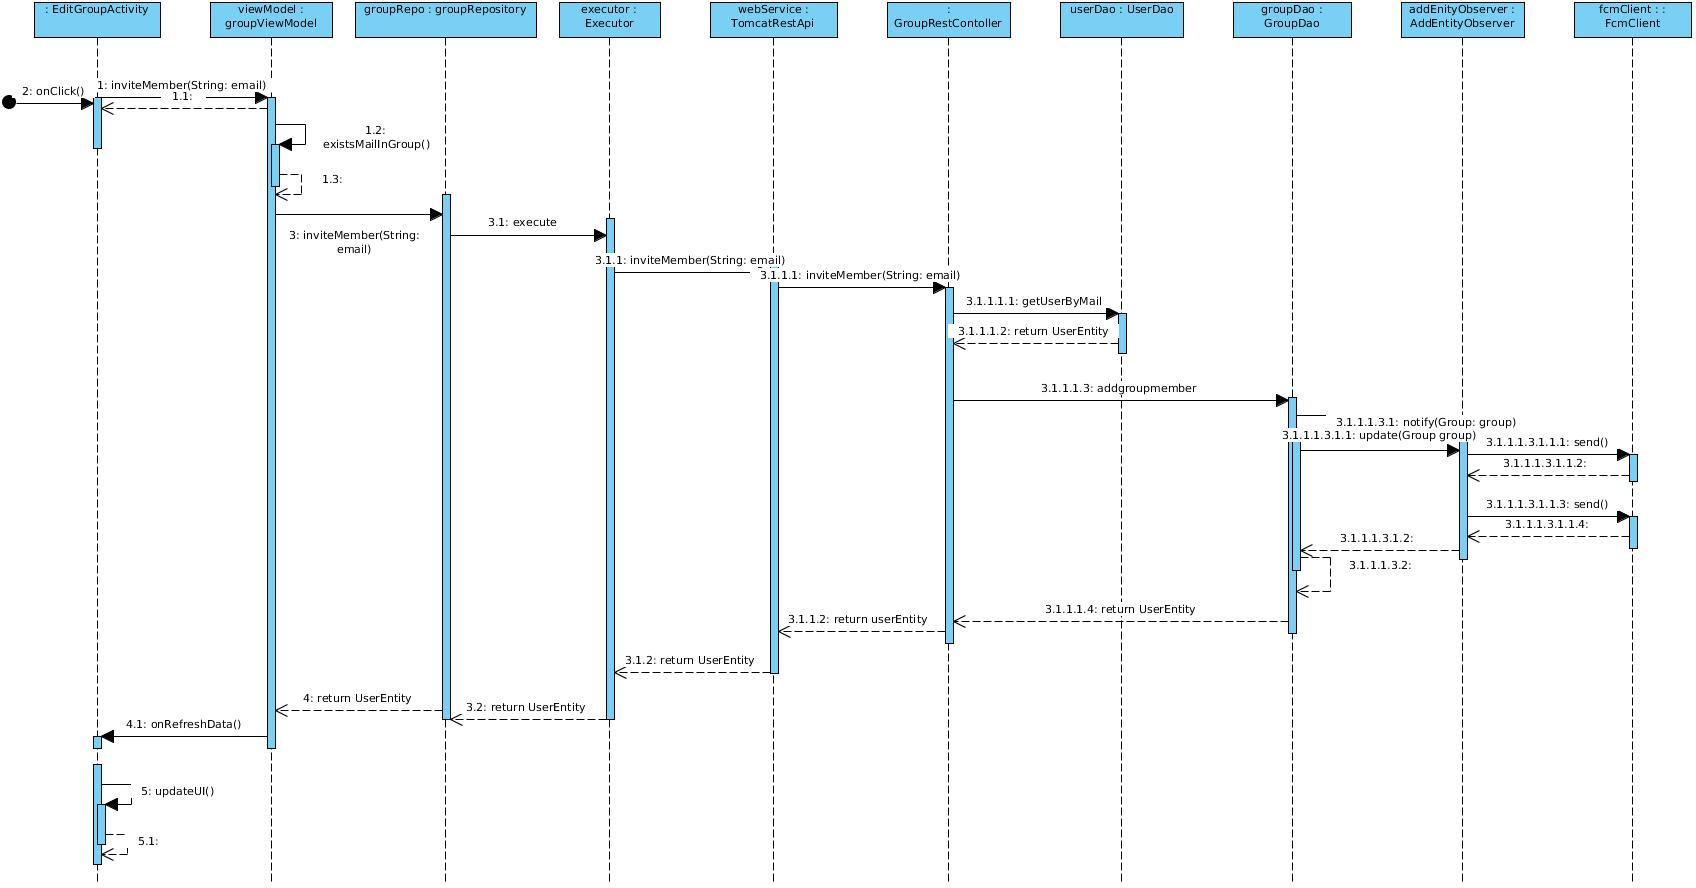
\includegraphics[width=1\textwidth]{../Sequenzdiagramme/addGroupMember.jpg}
	\caption{Sequenzdiagramm - Hinzufügen eines Gruppenmitglieds Teil 1}
\end{figure}

Das obige Sequenzdiagramm zeigt, was während der Ausführung des Programms passiert, wenn ein Benutzer die Funktion "inviteMember" ausführt. Das User Interface stellt dem Benutzer ein Textfeld zur Eingabe der E-Mailadresse und einen Button zum Bestätigen zur Verfügung. Bei Klick dieses Buttons extrahiert die Activity-Klasse die eingegebene Mail-Adresse aus dem Textfeld und übergibt diese an das ViewModel über den Methodenaufruf "inviteMember". Das ViewModel überprüft zunächst ob es bereits einen Benutzer in Gruppe gibt, der diese E-Mailadresse besitzt. Falls nicht, wird die Gruppeneinladung an die Grouprepository weitergeleitet und von dort über die Klasse TomcatrestApi an den Server gesendet.

Empfängt der Server eine Anfrage, einen User zu einer Gruppe hinzuzufügen, wird diese Anfrage zunächst an das UserDao weitergegeben. Dort wird zuerst die Methode getUserByMail() aufgerufen, um den richtigen Benutzer aus der Datenbank zu finden. Danach wird die addGroupmember-methode des GroupDaos aufgerufen. In dieser methode wird die neue gruppenanfrage in der Datenbank gespeichert und es werden die Observer benachrichtigt, dass sich Daten geändert haben.

Der AddEntityObserver erkennt, dass es sich um eine Änderung handelt, die seinen Veratnwortlichkeitsbereich betrifft. Er bekommt beim Aufruf der update()-Methode die Gruppe mit der zusätzlichen Gruppenanfrage übergeben. Der Observer extrahiert alle Gruppenmitglieder aus dem Gruppenobjekt und ruft die send()-methode des FcmClients auf, um das geänderte Gruppenobjekt an alle Gruppenmitglieder zu senden. Danach wird die send()-Methode ein zweites Mal aufgerufen, um dem neuen Gruppenmitglied die neue Gruppenanfrage zu übermitteln.

\begin{figure}[H]
	\centering
	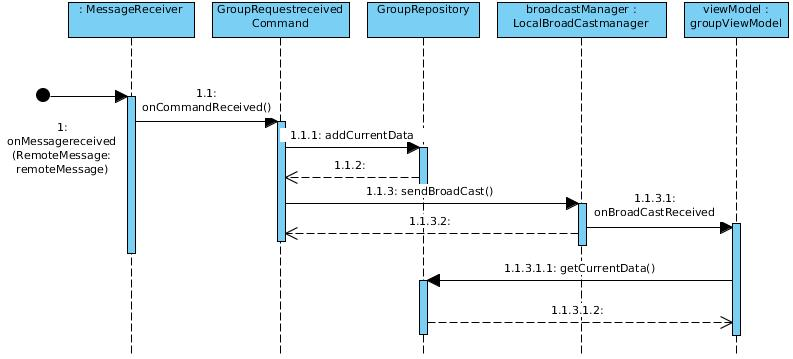
\includegraphics[width=1\textwidth]{../Sequenzdiagramme/addMember2.jpg}
	\caption{Sequenzdiagramm - Hinzufügen eines Gruppenmitglieds Teil 2}
\end{figure}

Das zweite Sequenzdiagramm zeigt, was passiert, wenn an einen Benutzer eine Gruppenmitgliedschaftsanfrage gesendet wird. Die Nachricht, die von dem Server, über dem Firebase Cloud Messaging Server, an den Client gesendet wird, löst einen Aufruf der Methode onMessageReceived() in der Klasse MessageReceiver aus. Diese Klasse extrahiert das JSON-Feld COMMAND\_CODE aus dem empfangenen JSON-Objekt und findet so heraus, an welches ServerCommand-Objekt die Anfrage weitergeleitet werden muss.

Nach Weiterleitung der Anfrage an den GroupRequestReceivedCommand wird dort das Datenfeld aus der JSON-Nachricht extrahiert. dort ist die Gruppe gespeichert, zu der er Benutzer eingeladen wurde. Diese Gruppe wird in dem öffentlichen "CurrentData" Field des GroupRepository gespeichert. Danach schickt das GroupRequestReceivedCommand-Objekt einen Broadcast an alle ViewModels. Das GroupViewModel erkennt, dass der Broadcast eine Änderung der Gruppen des Benutzers betrifft. Daher wird dort die onBroadcastReceived()-Methode auferufen. Daraufhin holt sich das ViewModel die aktualisierten Daten von der GoupRepository ab, durch einen Aufruf der getCurrentData()-Methode. Da das UI die LiveData der ViewModels beobachtet, wird automatisch bei einer Aktualisierung des ViewModels auch das UI aktualisiert und zeigt die neuen Daten an.

\subsection{Entfernen einer Gruppe}

\begin{figure}[H]
	\centering
	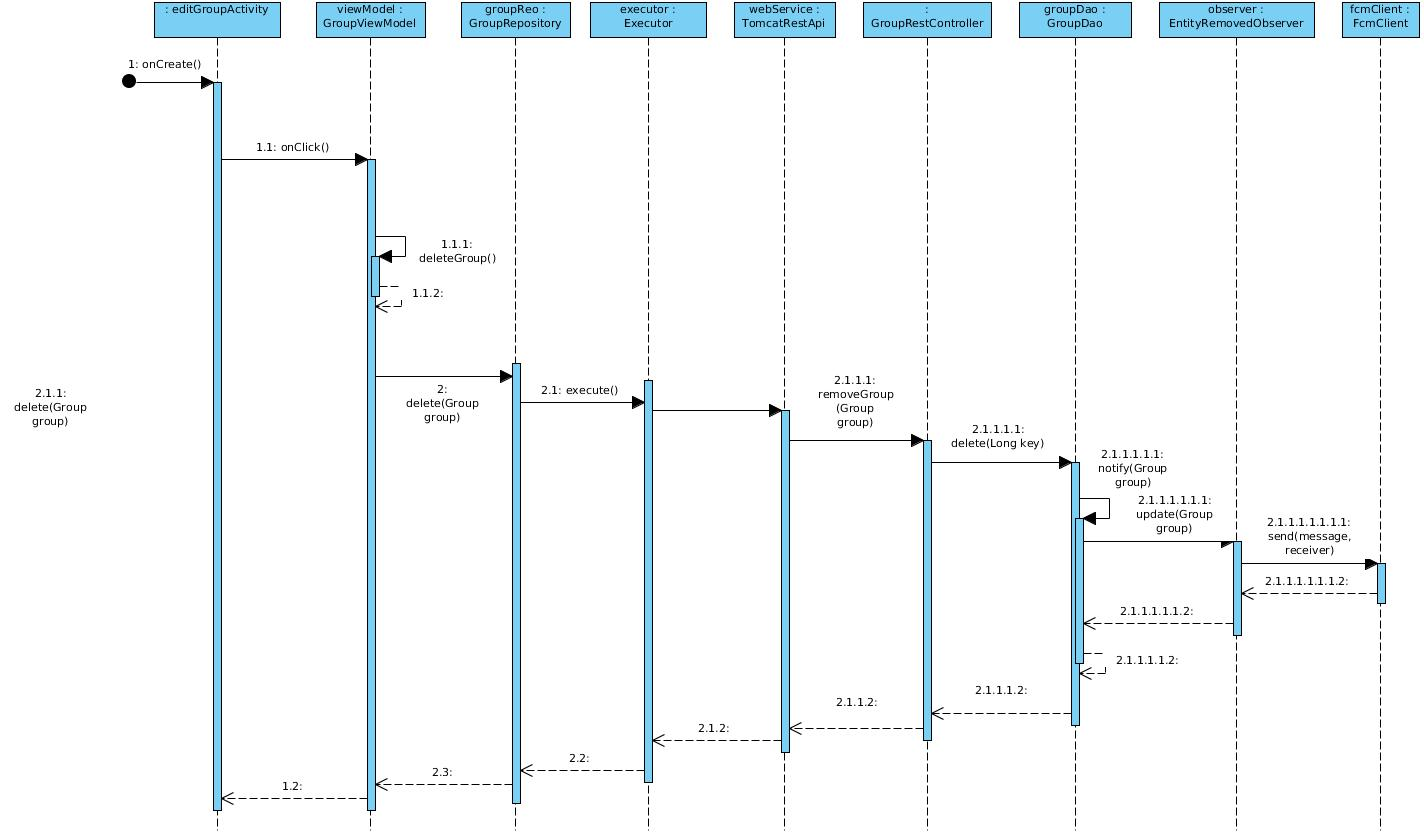
\includegraphics[width=1\textwidth]{../Sequenzdiagramme/deleteGroup_sequenz.jpg}
	\caption{Sequenzdiagramm - Entfernen einer Gruppe}
\end{figure}

Das obige Sequenzdiagramm zeigt den Programmablauf, nachdem ein Benutzer die "Gruppe löschen"-Funktion ausgelöst hat. Das UI gibt den Button Press an das GroupViewModel weiter. Dort wird die Gruppe zunächst in den lokaeln Daten gelöscht. Dabei muss sichergestellt werden, dass die Daten nach dem Löschen konsistent sind, also z.B. auch alle GOs der Gruppe gelöscht wurden.

Danahc wird die Anfrage über die GroupRepository und das Rest API an den Server übergeben, wo sie durch den Methodenaufruf deleteGroup() in der GroupRestController-Klasse ankommt. Von dort aus wird die Anfrage an das GroupDao gegeben, welches die Gruppe in der Datenbank löscht. Auch hier muss auf die Konsistenz der Daten geachtet werden. Danach werden die Observer des GroupDaos benachrichtigt, dass eine Ändeurng stattgefunden hat. Da die Änderung nur den EntityRemovedObserver betrifft, wird bei diesem Objekt die Methode update() aufgerufen. Mit dem Methodenaufruf wird auch die gelöschte Gruppe übergeben.

Der Observer baut ein Message-Objekt aus der erhaltenen Gruppe und extrahiert eine Listse aller Gruppenmitglieder aus dem Gruppenobjekt. Diese Daten werden witergegeben an dem FcmClient über die Methode send(). Dadurch werden die Nachrichten über die Löschung der Gruppe an die Gruppenmitglieder geschickt, damit diese ihre lokalen Daten anpassen können.

\section{Finish}{

}
% ------- textdoclet_include/finish.tex end

\end{document}
